%% ----------------------------------------------------------------
%% Thesis.tex -- MAIN FILE (the one that you compile with LaTeX)
%% ---------------------------------------------------------------

\pdfobjcompresslevel 0

\documentclass[utf8,12pt,a4paper,french, twoside]{thesis_template}

\makeglossaries

\newacronym{tdah}{TDAH}{Trouble du Déficit de l'Attention avec ou sans Hyperactivité}
\newacronym{nfb}{NFB}{neurofeedback}
\newacronym{es}{ES}{\textit{Effect Size}}
\newacronym{et}{ET}{Erreur Type}
\newacronym{est}{EST}{\textit{Effect Size} Total}
\newacronym{saob}{SAOB}{\textit{Systematic Analysis of Biases}}
\newacronym{eeg}{EEG}{électroencéphalogramme}
\newacronym{irb}{IRB}{\textit{Institutional Review Board}}
\newacronym{scp}{SCP}{\textit{Slow Cortical Potentials}}
\newacronym{tbr}{TBR}{Theta-Beta Ratio}
\newacronym{smr}{SMR}{Rythme Sensorimoteur}
\newacronym{iapf}{iAPF}{\textit{individualized Alpha Peak Frequency}}
\newacronym{emg}{EMG}{électromyogramme}
\newacronym{agcl}{AgCl}{Chlorure d'Argent}
\newacronym{au}{Au}{or}
\newacronym{wls}{WLS}{\textit{Weighted Multiple Linear Regression}}
\newacronym{lasso}{LASSO}{\textit{Least Absolute Shrinkage and Selection Operator}}
\newacronym{dt}{DT}{\textit{Decision Tree}}
\newacronym{wrss}{WRSS}{\textit{Weighted Residual Sum of Squares}}
\newacronym{ols}{OLS}{\textit{Ordinary Least Squares}}
\newacronym{mse}{MSE}{\textit{Mean Square Error}}
\newacronym{pblind}{PBlind}{\textit{Probably Blind}}
\newacronym{eog}{EOG}{Electro-Oculogramme}
\newacronym{mprox}{MProx}{\textit{Most Proximal}}
\newacronym{eo}{EO}{\textit{Eyes Open}}
\newacronym{cmi-mipdb}{CMI-MIPDB}{\textit{Child Mind Institute Multimodel Resource for Studying Information Processing in the Developing Brain}}
\newacronym{cmi-hbn}{CMI-HBN}{\textit{Child Mind Institute Healthy Brain Network}}
\newacronym{egi}{EGI}{\textit{Electrical Geodesics, Inc.}}
\newacronym{rpf}{RPF}{\textit{Riemannian Potato Field}}
\newacronym{srntbr}{srnTBR}{\textit{square-root normalized} TBR}

\begin{document}

% Title page

\begin{titlepage}

\vskip 1in

\begin{center}
{\LARGE Université de Paris} \\
\vskip 0in
\textbf{Ecole Doctorale Bio Borbonne Paris Cité ED 562} \\
\vskip 0in
\textbf{\textit{Hôpital Robert Debré}} \\
\vskip 0.3in

\Huge \textbf{Analyse statistique du Neurofeedback électroencéphalographique appliqué au Trouble du Déficit de l'Attention avec ou sans Hyperactivité}

\vskip 0.3in

%Sous titre de la thèse \\
%
%\vskip 0.7in

{\Large Par Aurore Bussalb} \\

\vskip 0.3in

{\large Thèse de doctorat de neurosciences} \\

\vskip 0.2in

{\large Dirigée par Richard Delorme} \\

\vskip 0.1in

{\normalsize Présentée et soutenue publiquement le} \\
\vskip 0.1in

\end{center}

Devant un jury composé de : % indiquer le jury complet sauf les examinateurs absents

Prénom Nom,  titre [ex. : Maître de conférence],  établissement, rôle par rapport à la thèse [ex : Rapporteur, Président ou encore directeur de thèse]

\begin{figure}[t]
	
\includegraphics[width=56.1mm]{logos/Logo_Universite_Paris.png} 
\end{figure}

\begin{figure}[b]
	
\includegraphics[width=108.2mm]{logos/creative_commons_pas_de_modifs.png} 
\end{figure}

\end{titlepage}

\pagebreak{\blankpage}
\pagebreak{\blankpage}

% Résumé en français, 4000 mots max 
% mots clés

\begin{center}
\MakeUppercase{\LARGE{R}\Large{esume de these}} \\
\vspace{0mm}
\noindent\rule{16cm}{0.4pt}
\end{center}


% une phrase d'accroche
Cette thèse porte sur le \glsfirst{nfb}-\glsfirst{eegi} appliqué au \gls{tdah} chez l'enfant dont l'efficacité et les facteurs d'amélioration sont 
étudiés ici en se basant d'une part, sur des données cliniques et d'autre part, sur les signaux électroencéphalographiques. 

% définitions
Le \gls{nfb} est une technique d'apprentissage à visée thérapeutique permettant 
de modifier un paramètre d'activité cérébrale, ici l'\gls{eeg}, au moyen d’un système de récompenses auditives et/ou visuelles 
délivrées instantanément via une interface de jeu sérieux. Cette technique a un large champ d'applications, cependant ici elle est uniquement étudiée 
dans le cadre du \gls{tdah} chez l'enfant. Le \gls{tdah} est un trouble neuro-développemental chronique communément traité par la prise de psychostimulants, 
mais dont le risque d'effets secondaires mène certains parents et pédopsychiatres à se tourner vers des approches non-médicamenteuses telles que le \gls{nfb}.
 
% problématique
Le \gls{nfb} appliqué au traitement du \gls{tdah} chez l'enfant a fait l’objet de nombreuses études ayant pour but de démontrer son efficacité. 
Cependant, elles n'ont pas encore permis d'atteindre de réel
consensus, ce qui pourrait s'expliquer par leurs divergences méthodologiques, cliniques et techniques. 

% méthodes
Ainsi l'objectif de cette thèse est, dans un premier temps, d'effectuer l'état des lieux du niveau de preuves de l'efficacité du \gls{nfb} pour les enfants \gls{tdah} grâce
à la réplication et à la mise à jour d'une récente méta-analyse sur le sujet. Dans un 
deuxième temps, l'hétérogénéité des études dans ce domaine est tournée à notre avantage afin de permettre 
l'identification des facteurs méthodologiques, cliniques et techniques qui pourraient avoir une influence sur la performance de ce traitement. Cette étape est réalisée
à l'aide de trois méthodes multivariées qui associent l'efficacité du \gls{nfb} aux facteurs d'intérêt. 
Les résultats de chacune de ces méthodes sont combinés afin de déterminer quels paramètres parmi ceux étudiés auraient effectivement un impact. 
Enfin, la pertinence de personnaliser le traitement par \gls{nfb} selon le profil \gls{eeg} des enfants, paramètre qui pourrait améliorer les résultats de ce traitement, est étudiée dans un troisième
temps à l'aide de méthodes de partitionnements appliquées à un marqueur \gls{eeg} couramment associé au \gls{tdah}. 

% résultats
La réplication et la mise à jour de la méta-analyse confirment les résultats obtenus par le passé sur davantage d'études : les évaluateurs non aveugles au traitement suivi par 
l'enfant notent une diminution significative des symptômes, à l'inverse de ceux qui sont aveugles. L'analyse des facteurs pouvant avoir une influence sur l'efficacité du \gls{nfb}
est en accord avec ce résultat et, par ailleurs, conclut qu'un traitement intensif est préférable. Enfin, personnaliser le traitement par \gls{nfb} semble pertinent étant donné que notre 
analyse de partitionnement a identifié deux groupes d'enfants \gls{tdah} selon leur profil \gls{eeg}.

% conclusion
Grâce à ces travaux, des facteurs d'amélioration du traitement par \gls{nfb} des enfants \gls{tdah} ont été mis en évidence afin de conduire à une efficacité accrue de ce traitement.




\large{\textbf{Mots-clés}} : \glsfirst{nfb}, \glsfirst{eeg}, \glsfirst{tdah}, meta-analyse, analyse de biais, partitionnement.
\thispagestyle{style5}

% Abstract 4000 words including spaces
% keywords

% Put the english title

\begin{center}
\MakeUppercase{\LARGE{A}\Large{bstract}} \\
\noindent\rule{16cm}{0.4pt}
\end{center}

\textbf{Title:} Statistical analysis of electroencephalographic Neurofeedback applied to Attention Deficit Hyperactivity Disorder

% une phrase d'accroche
This thesis deals with the \gls{eegic}-\glsfirst{nfb} applied to children with \gls{adhd} whose efficacy and factors for 
improvement are studied thanks to clinical data and \gls{eegic} signals.

% définitions
\gls{eegic}-\gls{nfb} is a learning technique with a therapeutic purpose that enables to modify the \gls{eegic} activity 
as part of a conditioning paradigm that presents auditive and/or visual rewards via a serious gaming interface.
This technique has a lot of applications. This work specifically focuses on its therapeutic use for children with \gls{adhd}.
This neurodevelopmental disorder is characterized by an attention deficit disorder and/or a motor hyperactivity that
negatively impact the well being of children. The medication treatment is commonly prescribed because of its efficacy but
it can cause side effects, that's why some parents and child psychiatrists choose non-medication approaches such as \gls{eegic}-\gls{nfb}, simply noted 
\gls{nfb}. 

% problématique
\gls{nfb}, as a treatment for children with \gls{adhd}, bas been subject to various studies to prove its efficacy. 
However, they have not yet reached a consensus, which could be explained by the small number of included patients, but also by
the clinical, technical and methodological discrepancies of the studies.  

% methodes
Thus, the first purpose of this thesis is to assess the level of evidence of the \gls{nfb} efficacy for children with \gls{adhd}
through the replication and the update of a meta-analysis on this topic. 
The replication aims at settling certain debates surrounding some methodological choices of the author. 
The update of the meta-analysis enables to include more studies that, despite the assumption regarding their homogeneity, 
differ from each other in terms of population and methods.

Then, this heterogeneity is studied in order to identify methodological, clinical, and technical factors that would influence
the performance of this treatment. This step is carried out thanks to three multivariate regression methods that link \gls{nfb} 
efficacy to the factors of interest. Results of each method are combined in order to determine which parameter among those
studied would indeed have an impact. 

However, some innovative factors cannot be included in this analysis because too few studies report on their performance.
Thus, the last step of this work is to analyze the relevance of personalizing the \gls{nfb} treatment based on children \gls{eegic} profil
thanks to clustering methods applied to an \gls{eegic} marker commonly linked with \gls{adhd}.

% résultats
The replication and update of the meta-analysis confirm previous results on more studies: raters who are not blind to the treatment
followed by the child observe a significant decrease of symptoms contrary to blind raters for reasons that may be more complex 
than it appears. This result is confirmed by the analysis of factors that could influence the \gls{nfb}, which also identifies 
treatment intensity. Eventually, personalizing \gls{nfb} treatment seems relevant since the clustering analysis finds two groups
of \gls{adhd} children with distinct \gls{eegic} phenotypes. 

% conclusion
To conclude, this work contributes to bring answers regarding \gls{nfb} efficacy by replicating and updating a meta-analysis as well 
as studying blind raters' assessments. Furthermore, this works enabled to determine parameters whose definition or presence may improve
\gls{nfb} efficacy.

\large{\textbf{Keywords}} : \glsfirst{nfb}, \glsfirst{eegy}, \glsfirst{adhd}, meta-analysis, bias analysis, clustering.
\thispagestyle{style5}

%\pagebreak{\blankpage}

\newpage
\topskip0pt
\vspace*{\fill}
 
\begin{flushright}
\textit{A mon cher grand-père, René Marty.}
\end{flushright}

\vspace*{\fill}
\thispagestyle{empty}

\newpage
\begin{center}
\MakeUppercase{\LARGE{R}\Large{emerciements}} \\
\noindent\rule{17cm}{0.4pt}
\end{center}
%\thispagestyle{empty}

%\pagebreak{\blankpage}

\tableofcontents
\thispagestyle{style2}

\listoffigures
\thispagestyle{style3}
\newpage

\listoftables

\newpage
\printglossary[title=Abréviations, type=\acronymtype, nonumberlist, style=long]

\newpage
\chapter{Introduction} \label{chapitre-1}

% voir thèse d'alexandre pouch
% composante totale
% aller dans les détails
% dopamine
% Enriqure 2017 et Strehl 2014 (-> threshold)
% voir Rogala2016
% plasticité cérébrale

Les concepts sur lesquels porte le travail décrit dans ce manuscrit sont définis dans cette première partie introductive. Tout d'abord, la technique du \gls{nfb}-\gls{eeg}, 
qui est au centre de ce travail, est présentée en détail, puis ses diverses applications sont listées. Dans la suite du manuscrit, seule l'une d'entre elles est étudiée : 
il s'agit du \gls{tdah} chez l'enfant, dont les principales caractéristiques sont exposées dans cette partie. 

Une fois ces concepts décrits, les objectifs de cette thèse sont énoncés et la contribution de chaque chapitre est mise en évidence. Enfin, les analyses 
présentées dans ce manuscrit ont fait l'objet de publications scientifiques et d'une communication orale dont les références sont fournies à la fin de ce chapitre. , 

\clearpage 

\section{Définition du Neurofeedback}

Le \gls{nfb} est une technique d’apprentissage à visée thérapeutique permettant de modifier un paramètre d’activité cérébrale au moyen d’une 
information en temps réel associée à une récompense \citep{Arns2014}. L'activité cérébrale qui nous intéresse ici est l'\gls{eeg}, dont les caractéristiques sont tout d'abord
rappelées. Ensuite, la découverte et l'évolution de la méthode du \gls{nfb}-\gls{eeg} sont retracées, puis son principe est décrit précisément.

\subsection{Acquisition de l'électroencéphalogramme} \label{eeg_definition}

L'\gls{eeg} est un examen électrophysiologique du cerveau, non invasif, permettant d’enregistrer de manière amplifiée l'activité électrique du cerveau \citep{Nunez2006}. 

\subsubsection{Génération de l'\gls{eeg}}

Cette activité cérébrale est enregistrée grâce à des électrodes placées sur le scalp qui détectent la sommation de l'activité électrique d'un grand nombre de neurones actifs de manière synchrone.
Cette activité électrique est générée par les potentiels post-synaptiques dans les dendrites apicaux des cellules pyramidales du cortex \citep{Hallez2007}. Le cortex désigne 
la substance grise périphérique des hémisphères cérébraux, il se compose de six souches qui comportent différents types de neurones : les cellules pyramidales à l'origine de l'\gls{eeg} 
se situent dans les couches III et V (la sixième étant la plus profonde). Ces cellules sont d'excellents dipôles électriques grâce à leur longue dendrite apicale perpendiculaire 
à la surface corticale \citep{Bekkers2011}. 

\subsubsection{Rythmes cérébraux}

L'\gls{eeg} est un signal de très faible amplitude (de l'ordre de 50$\mu$V), elle est d'ailleurs proportionnelle au degré de synchronisation des neurones pyramidaux \citep{Hallez2007}. 
Ainsi, en fonction de l'activité de ces neurones, différents rythmes cérébraux vont être présents sur l'\gls{eeg}. 

Les rythmes cérébraux correspondent à des oscillations électromagnétiques dans une bande de fréquence donnée, dont les bornes peuvent varier selon les études et sont présents sur l'\gls{eeg}
selon l'état psychologique d'un sujet \citep{Marzbani2016} :  
\renewcommand{\labelitemi}{$\bullet$}
\renewcommand{\labelitemii}{$\cdot$}
\begin{itemize}
\item \emph{les ondes delta} (moins de 4Hz) : observées lorsqu'un grand nombre de groupes de neurones est synchrone, c'est à dire pendant le sommeil profond,
\item \emph{les ondes theta} (4-8Hz) : observées durant un état de somnolence, sous hypnose ou lors de la mémorisation d'informations par exemple,
\item \emph{les ondes alpha} (8-12Hz) : observées notamment durant un état de relaxation les yeux fermés,
\item \emph{les ondes beta} (12-30Hz), dont les ondes \gls{smr} entre 12 et 15Hz : observées durant un état d'attention et de vigilance mentale par exemple,
\item \emph{les ondes gamma} (30-100Hz) : observées en particulier durant l'apprentissage.
\end{itemize}

Afin d'interpréter la présence de ces rythmes cérébraux sur l'\gls{eeg}, il faut prendre en considération la zone sur laquelle ils sont observés 
car chaque aire cérébrale a des fonctions spécifiques, comme par exemple \citep{Marzbani2016} :
\begin{itemize}
\item \emph{la zone frontale} est impliquée dans la mémoire et la concentration,
\item \emph{la zone temporale} est impliquée dans le langage et la lecture,
\item \emph{la zone occipitale }est impliquée dans l'apprentissage visuel,
\item \emph{la zone pariétale} est impliquée dans la résolution de problèmes,
\item \emph{la zone centrale} est impliquée dans l'attention.
\end{itemize}

Ces différentes fonctions sont résumées à la Figure~\ref{Figure:introduction_cortical_areas_and_functions} où les principales électrodes, placées en accord avec le système \gls{eeg} 10-20 
défini par la suite, sont représentées ainsi que les aires cérébrales qu'elles couvrent. 

\begin{figure}[h!]
  \centering
	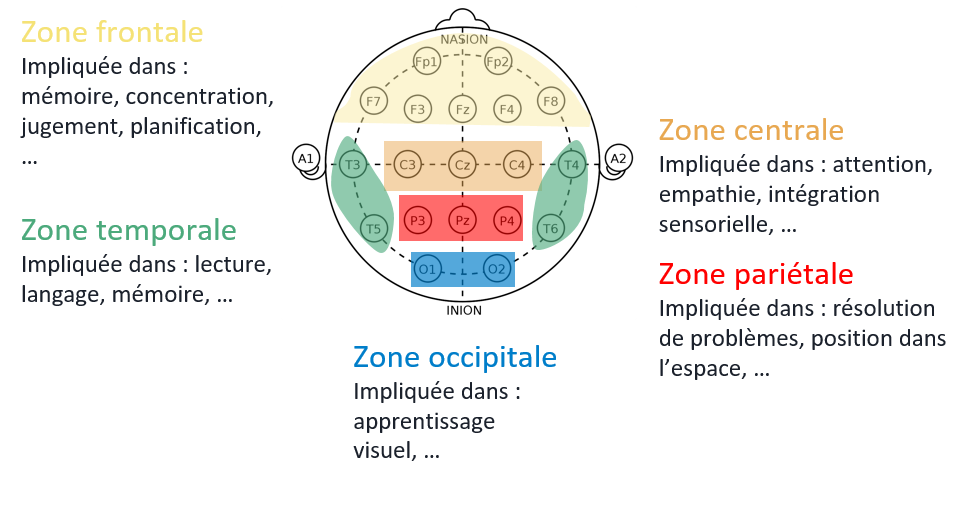
\includegraphics[width=1\linewidth]{figures/chapter-1/introduction-cortical-areas-and-functions} 
  \caption{Représentation des aires cérébrales avec des exemples de leurs fonctions. Les principales électrodes du système international 10-20 sont également présentées.}
  \label{Figure:introduction_cortical_areas_and_functions}
\end{figure}

\subsubsection{Enregistrement de l'\gls{eeg}}

L'\gls{eeg} est enregistré sur le cuir chevelu à l'aide d'électrodes dont le nombre et le placement varient en fonction de ce qu'on cherche à observer.
Le placement des électrodes suit généralement le système international 10-20 qui a été mis en place en 1948 afin d'harmoniser les enregistrements à travers le monde 
\citep{Jasper1949, Sharbrough1991} et qui est représenté à la Figure~\ref{Figure:introduction_system_10_20}.

\begin{figure}[h!]
  \centering
	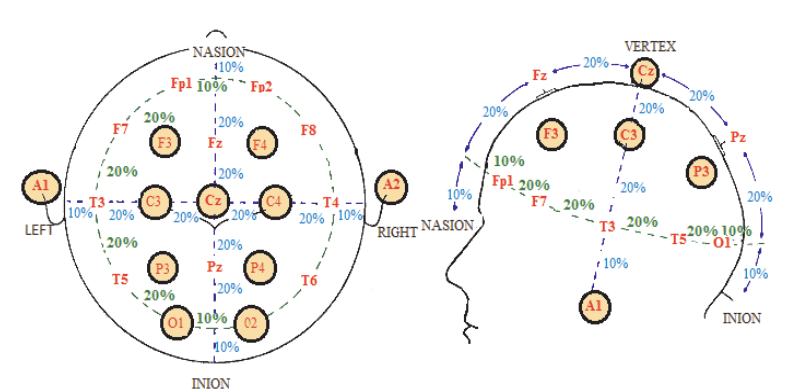
\includegraphics[width=1\linewidth]{figures/chapter-1/introduction-system-10-20} 
  \caption{Placement des électrodes enregistrant l'\gls{eeg} suivant le système international 10-20. Les pourcentages sont calculés par rapport à la distance totale entre le nasion
	et l'inion, et par rapport à la distance totale entre les mastoïdes gauche et droit (A1 et A2). Les électrodes les plus couramment utilisées 
	sont cerclées de noir sur fond beige \citep{Marzbani2016}.}
  \label{Figure:introduction_system_10_20}
\end{figure}

Le système 10-20 couvre l'ensemble des aires cérébrales du cortex, en répartissant les électodes de manière régulière entre les points de repère de la tête : le nasion, le vertex et l'inion. 

Comme on peut le voir sur les Figures~\ref{Figure:introduction_system_10_20} et \ref{Figure:introduction_cortical_areas_and_functions}, le nom des électrodes est 
constitué d'une lettre et d'un chiffre ou de la lettre z, cette nomenclature est définie par \citet{Jasper1949} :
\begin{itemize}
\item la lettre renseigne la position de l'électrode sur le scalp : F, T, C, P et O correspondent respectivement aux régions Frontale, Temporale, Centrale, Pariétale et Occipitale,
\item le chiffre indique quant à lui si l'électrode est placée sur l'hémisphère droit (chiffre pair) ou sur l'hémiphère gauche (chiffre impair),
\item la lettre z est associée aux électrodes qui se trouvent sur la ligne médiane du crâne,
\item les électrodes Fp sont situées en pré-frontal,
\item les électrodes A1 et A2 sont généralement des électrodes de référence.
\end{itemize}
  
Le nombre et le placement des électrodes varie selon le but de l'application de l'\gls{eeg} : par exemple enregister l'\gls{eeg} afin
de mener une localisation de sources (c'est à dire déterminer les sources corticales à l'origine de l'\gls{eeg}) demande une forte densité spatiale \citep{Lantz2003}. 

Par ailleurs, le type des électrodes d'enregistrement peut également être différent : 
alors que les électrodes à gel sont considérées comme le \textit{gold standard}, l'utilisation des électrodes sèches se répand de plus 
en plus du fait notamment de leur facilité d'utilisation. Cependant, leur fiabilité n'est pas encore parfaitement démontrée \citep{Lopez2014}. 

Ce qui différencie les électrodes sèches des électrodes à gel est notamment la valeur de l'impédance qui, lorsqu'elle est faible, rend compte du bon contact entre la peau et les électrodes \citep{Lopez2014}. 
L'impédance est généralement obtenue en envoyant un faible courant de 10Hz entre 2 électrodes et en mesurant l'opposition à ce flux de courant \citep{Kappenman2010}. La peau du crâne est 
couverte par des cellules de peau morte qui conduisent à une forte impédance.
Ainsi, pour la diminuer, les électrodes à gel sont imprégnées d'un électrolyte qui facilite la tranduction des courants ioniques. Toutefois, l'utilisation de ce type d'électrodes 
n'exclut pas la mesure de l'impédance qui doit être faible \citep{Lopez2014}. En général, en l'absence de gel conducteur, l'impédance se
situe entre 150 et 200 k$\Omega$ et tombe entre 5 et 10K$\Omega$ après application du gel \citep{Lopez2014}. Une faible impédance signifie 
que le niveau de bruit dans le signal est réduit \citep{Kappenman2010}.

Enfin, afin d'obtenir le tracé des signaux \gls{eeg} présenté à la Figure~\ref{Figure:introduction_eeg_example}, ceux-ci sont amplifiés 
à l'aide d'un amplificateur, qui peut être conforme à la norme ISO-60601-2-26 \citep{ISO}. 

\begin{figure}[h!]
  \centering
	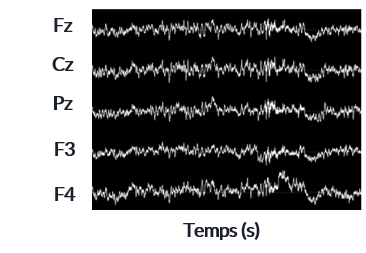
\includegraphics[width=0.5\linewidth]{figures/chapter-1/introduction-eeg-example} 
  \caption{Exemple d'\gls{eeg} réel enregistré sur 5 secondes. }
  \label{Figure:introduction_eeg_example}
\end{figure}

\subsection{Exemples d'application de l'électroencéphalogramme}

L'\gls{eeg} a diverses applications : il peut être analysé en temps réel dans le cadre, par exemple, de l'épilepsie, du suivi d'une personne dans 
le coma ou d'un enfant prématuré et des interfaces cerveau machine (\gls{bci} en anglais) \citep{Li2010}. De plus il 
est également utilisé dans le milieu de la recherche notamment pour la localisation de sources \citep{Latif2006}.

Dans le cadre de cette thèse, l'\gls{eeg} est analysé en temps réel durant l'entrainement par \gls{nfb} défini précisément par la suite.  
 

\subsection{Historique du Neurofeedback}

Les prémices du \gls{nfb} remontent au début des années 1930, peu après l'enregistrement du premier \gls{eeg} humain et de la découverte des ondes alpha par Hans Berger en 1929 \citep{Berger1929}.
En effet, \citet{Durup1935} et \citet{Loomis1936} ont observé que les ondes alpha de l'\gls{eeg}, oscillant entre 8 et 12Hz, pouvaient être contrôlées grâce au 
conditionnement classique \citep{Pavlov1929}. Ce conditionnement, également appelé conditionnement répondant ou pavlovien, consiste à apprendre un comportement en associant un stimuli
de l'environnement à des réactions automatiques de l'organisme.

Plus tard, ce qui peut être considéré comme le premier entrainement par \gls{nfb} a été mené par le Dr. Kamiya qui, en se basant sur les travaux de \citet{Durup1935}, 
a demandé aux sujets de son étude de contrôler le rythme alpha à l'aide d'un retour auditif \citep{Kamiya1969}, ce qu'ils ont réussi à faire. 

Une preuve solide de la modulation de l'\gls{eeg} a été rapportée dans les années 1960 par le Dr. Sterman et son équipe \citep{Sterman1969} : l'expérience 
originelle consistait à entrainer le cerveau des chats en leur apprenant quoi faire pour obtenir de 
la nourriture. En effet, les chats devaient dans un premier temps actionner un levier pour remplir leur bol de nourriture. Ensuite, une fois cette étape maitrisée, 
l'expérience s'est complexifiée avec l'ajout d'un son qui, lorsqu'il retentissait, empêchait les chats d'obtenir leur nourriture lorsqu'ils appuyaient sur le levier.
Une fois le silence revenu, le chat pouvait à nouveau recevoir de la nourriture en actionnant le levier.  

C'est durant cette phase de son expérience, au moment où le chat attend la fin du son, que le Dr. Sterman a extrait un rythme particulier au niveau de leur cortex sensorimoteur : 
le \gls{smr}, qui correspond aux fréquences entre 12 et 15Hz. Ensuite, le but du Dr. Sterman a été d'entrainer les chats à produire ce rythme en leur donnant de la nourriture, non plus grâce 
au levier, mais lorsqu'ils réussissaient à l'émettre pendant une demi seconde, ce que les chats ont vite appris à faire. Cette expérience a été la première à montrer que le comportement
du cerveau pouvait être affecté par la modulation de l'\gls{eeg}. 

Peu de temps après, le Dr. Sterman a été approché par la NASA pour évaluer la toxicité du carburant utilisé pour les fusées, connu pour son risque de provoquer de violentes crises
d'épilepsie, sur les astronautes. Afin de mettre en évidence son effet épileptogène, ce carburant a été testé sur des chats parmi lesquels ceux qui avaient précédemment appris 
à moduler leur \gls{smr}. Comme attendu, au contact de ce carburant, les chats
ont souffert de convulsions, mais les chats ayant participer à l'expérience du \gls{smr} ont présenté moins de crises ou ont eu une meilleure tolérance aux effets nocifs du carburant \citep{Sterman1974}.  
Cette expérience a permis de démontrer que le contrôle de l'activité cérébrale pouvait être associé à des bénéfices cliniques, ouvrant ainsi la voie aux expériences incluant les humains.

En 1972, une patiente épileptique a entrainé son \gls{smr} grâce à la technique du \gls{nfb} : elle a réussi à moduler son \gls{smr}, conduisant à la quasi-disparition de ses crises 
d'épilepsie durant les séances \citep{Sterman1974}. 

Alors que l'épilepsie a été la première application du \gls{nfb}, un autre usage thérapeutique possible commence à être étudié dans la foulée : le \gls{tdah} chez l'enfant \citet{Lubar1976ADHD}. 
Cette étude est divisée en trois phases : tout d'abord, l'enfant module les ondes cérébrales d'intérêt dans le bon sens, puis ensuite dans le sens inverse et enfin à nouveau dans le bon sens.
Des résultats encourageants sont observés.

A la suite de ces observations prometteuses, d'autres chercheurs se sont penchés sur cette technique, cependant, faute d'une technologie suffisamment puissante, il leur était impossible
d'obtenir des preuves cliniques plus solides. C'est pourquoi, après les années 80, le \gls{nfb} est tombé en désuétude \citep{Masterpasqua2003}.
 
Il faut attendre les années 2000 pour que la communauté scientifique et médicale s'intéresse de nouveau sérieusement au \gls{nfb}, conduisant à une explosion du nombre d'articles scientifiques publiés 
visant à mieux comprendre ses effets, illustrée à la Figure~\ref{Figure:introduction_number_of_nfb_publications}. 

\begin{figure}[h!]
  \centering
	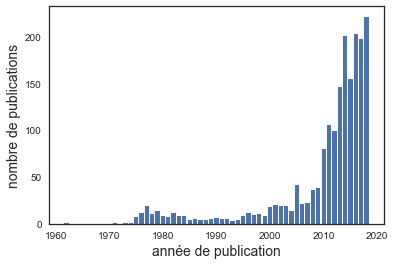
\includegraphics[width=0.7\linewidth]{figures/chapter-1/introduction-number-of-nfb-publications} 
  \caption{Evolution du nombre de publications sur le \gls{nfb} par année, entre 1962 et 2018. La base de données PubMed a été questionnée avec les 
	termes de recherche "Neurofeedback OR EEG Biofeedback".}
  \label{Figure:introduction_number_of_nfb_publications}
\end{figure}

Les dates clés de l'histoire du \gls{nfb} sont résumées à la frise présentée à la Figure~\ref{Figure:introduction_nfb_history}.

\begin{figure}[h!]
  \centering
	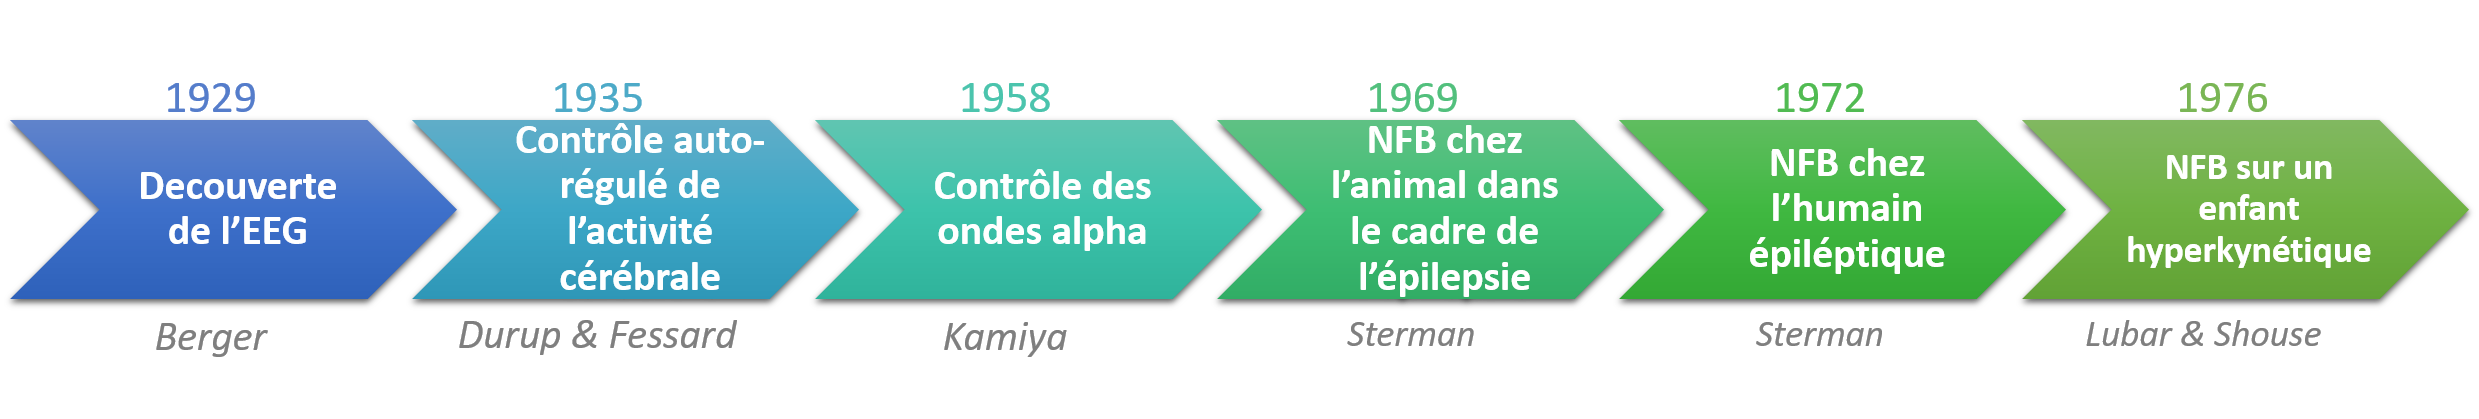
\includegraphics[width=1\linewidth]{figures/chapter-1/introduction-nfb-history} 
  \caption{Dates clés de l'histoire du \gls{nfb}.}
  \label{Figure:introduction_nfb_history}
\end{figure}

\subsection{Principe du Neurofeedback} \label{principe_nfb}

\subsubsection{Définition du \gls{nfb}}

Le \gls{nfb} a pour but d'apprendre à un sujet à auto-réguler son activité cérébrale à l'aide de retours auditifs et/ou visuels en temps réel
intégrés dans un jeu sérieux \citep{Wang2010}. Ces retours lui permettent de suivre la régulation de son rythme cérébral : s'il est modulé de 
la manière souhaitée, une récompense auditive et/ou visuelle est attribuée, sinon le sujet doit prendre une action corrective. 

Le \gls{nfb} est basé sur le conditionnement opérant \citep{Reynolds1975} où le conditionnement n'est pas lié à 
des réponses réflexes de l'organisme, comme c'est le cas pour le conditionnement classique, mais à l'influence de l'environnement, qui 
renforce positivement ou négativement le conditionnement \citep{Skinner1948}. 

L'activité cérébrale enregistrée lors du \gls{nfb} est couramment l'\gls{eeg} dont les caractéristiques sont décrites en \ref{eeg_definition}.
Cependant d'autres modalités telles que l'imagerie par résonance magnétique fonctionnelle (\gls{fmri} en anglais) sont parfois utilisées \citep{Sulzer2013}. 

Le \gls{fmri} mesure la réponse \gls{bold}, c'est à dire les différences du signal dues à des changements locaux de la concentration d'hémoglobine désoxygénée 
dans le tissu cérébral qui est dépendante de l'activité neuronale \citep{Dewiputri2013}. Dans le cas du \gls{fmri}-\gls{nfb}, c'est à partir du signal 
\gls{bold} que le \textit{feedback} est calculé \citep{Dewiputri2013}. 

Alors que l'\gls{eeg} possède une résolution temporelle élevée, sa résolution spatiale est quant à elle faible, 
contrairement au \gls{fmri}. Ainsi des études ont mis en place un couplage de ces deux modalités pour pallier leurs faiblesses et conduire à des 
protocoles de \gls{nfb} plus efficaces \citep{Perronnet2017}. 

Cependant, bien que prometteur ce couplage est difficile à mettre en place, notamment à cause du feedback \cgls{fmri}.
Un couplage plus souvent observé est celui entre l'\gls{eeg} et l'\gls{emg} : cette fois-ci le sujet doit réguler son activité cérébrale en même temps que son
activité musculaire et est donc récompensé sur les deux \citep{Bink2014}.

Dans la suite de cete thèse, seul le \gls{nfb}-\gls{eeg}, simplement noté \gls{nfb}, est étudié. 

\subsubsection{Etapes de l'entrainement par \gls{nfb}}

Le \gls{nfb} est un entrainement cognitif en boucle fermée : une représentation de l'activité cérébrale est retournée en temps réel
au sujet afin de l'aider à la réguler \citep{Enriquez2017}. Cet entrainement s'effectue en cinq temps \citep{Enriquez2017}, détaillés
par la suite :
\begin{enumerate}
\item l'acquisition du signal \gls{eeg}, 
\item le pré-traitement en temps réel du signal,
\item l'extraction des marqueurs d'intérêt du signal qui doivent être modulés par le sujet (les neuromarqueurs),
\item la génération du \textit{feedback},
\item le sujet module son activité, en adpatant sa stratégie en fonction du retour qu'il a reçu. 
\end{enumerate}

La première étape consiste à \emph{enregistrer l'\gls{eeg} }comme expliqué précédemment dans la partie \ref{eeg_definition}. Le choix
du nombre et du placement des électrodes se fait en fonction de l'application du \gls{nfb}, dont les principales sont décrites en
\ref{applications_NFB}. 

Le signal \gls{eeg} étant de faible amplitude, il est très facilement perturbé par des artefacts d'origine physiologique (générés par le
corps du patient) et d'origine environnementale. Les artefacts physiologiques les plus couramment observés sont les clignements et mouvements
d'yeux \citep{Iwasaki2005} et les artefacts musculaires causés par exemple par des mouvements du visage ; les artefacts environnementaux sont le plus souvent 
dus aux lignes électriques (50Hz en Europe et 60Hz aux Etats-Unis). 

Ces artefacts se superposent à l'activité électrique du cerveau pouvant fausser l'extraction du marqueur d'intérêt et donc rendre
incorrect le \textit{feedback} délivré \citep{Enriquez2017}. C'est pourquoi des \emph{méthodes de rejet ou de correction d'artefacts} en temps 
réel sont implémentées pour s'assurer que les récompenses sont bien calculées à partir du signal \gls{eeg} et non sur du bruit. 

Les méthodes de rejet consistent à ne pas extraire de marqueur d'intérêt d'un segment artefacté d'une durée donnée de l'\gls{eeg} (appelée époque). Pour sélectionner
les époques à garder, certaines études définissent un seuil sur l'amplitude du signal : si l'amplitude du signal d'une époque est supérieure
à ce seuil, cette époque est rejetée \citep{Gevensleben2009, Heinrich2004}. La valeur de ce seuil peut être fixe ou adaptative et peut 
différer ou non selon les canaux. 

D'autres études se basent sur la géométrie Riemannienne pour rejeter les époques artefactés \citep{Barthelemy2019, Bioulac2019}. 
la matrice de covariance de chaque segment, dont l'équation est donnée en équation Eq.~(\ref{eq:introduction_covariance_matrix}), est calculée pour un sous-ensemble de canaux : les 
segments dont la matrice de covariance se retrouve à l'extérieur d'une région d'acceptabilité définie grâce à une référence d'\gls{eeg} propres sont alors rejetés.

\begin{equation}
\label{eq:introduction_covariance_matrix}
\Sigma = \frac{1}{N - 1}XX^T,
\end{equation}
avec $X$ une matrice ($C \times N$) correspondant à une époque du signal \gls{eeg}, avec $N$ le nombre d'échantillons temporels et $C$ le nombre de canaux. 

Dans le cas où des artefacts sont détectés, l'utilisateur peut en être informé et adopter une action corrective, à l'instar de ce qui est implémenté dans 
\citet{Bioulac2019}.

Dans certains cas, les artefacts oculaires ne sont pas rejetés, mais sont corrigés en temps réel \citep{Barthelemy2017, Maurizio2014, Bioulac2019} en se basant sur
le principe de la séparation aveugle de sources (la \gls{bss} en anglais). Les signaux \gls{eeg} sont le résultat d'un mélange de sources cérébrales et non cérébrales : le but 
de la \gls{bss} est d'estimer ces sources à partir des signaux et d'identifier la source qui correspond à l'artefact oculaire pour la supprimer.
% équatiosn ? plus de précisions ?

En ce qui concerne les artefacts électriques, ils sont corrigés à l'aide d'un filtre coupe-bande qui supprime le 50 ou 60Hz \citep{Bioulac2019}.

Ensuite, la troisième étape consiste à \emph{extraire le marqueur à moduler} lors de la session de \gls{nfb}, appelé par la suite neuromarqueur : 
celui-ci, tout comme les électrodes utilisées, dépend de l'application du \gls{nfb}. 

Le neuromarqueur correspond le plus souvent aux ondes cérébrales listées en \ref{eeg_definition}, isolées au 
niveau de certaines électrodes. Dans certains cas, le neuromarqueur est un ratio de deux ondes cérébrales \citep{Gevensleben2009}. 

Les caractéristiques de l'\gls{eeg} étant différentes d'un sujet à l'autre, notamment à cause de l'âge, de la présence d'une maladie, de la capacité à effectuer une tâche ou du volume 
du cerveau \citep{Enriquez2017, Klimesch1999, Moretti2004, Alkoby2017}, la personnalisation des bandes de fréquence est parfois proposée par les applications de \gls{nfb}. 
En effet, il est supposé qu'adapter la définition des bandes de fréquence au sujet conduira à une meilleure efficacité \citep{Enriquez2017}. 

Une façon de personnaliser les bandes de fréquence est de se baser sur la fréquence du pic alpha du sujet \citep{Alkoby2017, Escolano2014, Bazanova2018, Bioulac2019}, qui 
est propre à chaque individu \citep{Haegens2014, Aurlien2004, Smit2006}. Un exemple de ce pic est présenté à la Figure~\ref{Figure:introduction_iapf}.

\begin{figure}[h!]
  \centering
	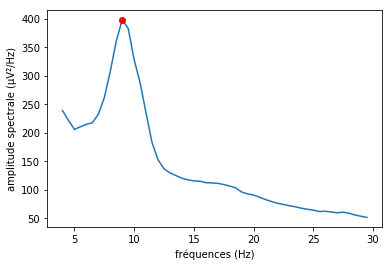
\includegraphics[width=0.7\linewidth]{figures/chapter-1/introduction-iapf} 
  \caption{Spectre d'un signal \gls{eeg} obtenu les yeux fermés au repos. L'\gls{iapf} correspond au point rouge.}
  \label{Figure:introduction_iapf}
\end{figure}

Enfin, certaines applications de \gls{nfb} proposent d'entrainer le neuromarqueur qui correspond le mieux au profil \gls{eeg} du sujet 
\citep{Bioulac2019, Kerson2013}, comme expliqué dans le cas du traitement du \gls{tdah} décrit en \ref{nfb_and_adhd}. 

Une fois le neuromarqueur extrait, l'étape suivante est de \emph{délivrer le feedback au sujet}. Pour ce faire, la valeur du neuromarqueur est comparée à un seuil
qui peut être fixe ou adaptatif, défini manuellement ou automatiquement \citep{Arns2014}.

En effet, le seuil peut être fixe tout au long de la session \citep{Kropotov2005, Monastra2002}, ou bien évoluer entre les sessions ou au sein même d'une session \citep{ 
Christiansen2014}. Utiliser un seuil incrémental a pour but d'adapter les récompenses octroyées au sujet en fonction de ses performances et 
de le garder motivé \citep{Bauer2016, Lansbergen2011}. 

Le \textit{feedback} présenté au sujet dépend donc du résultat de la comparaison entre la valeur du neuromarqueur et celle du seuil. Par ailleurs, en fonction du temps durant lequel
le neuromarqueur est modulé comme souhaité, les récompenses peuvent varier \citep{Bioulac2019}. 

Enfin, en fonction du feedback qu'il reçoit, le \textit{sujet va moduler son activité cérébrale} dans la direction attendue, en appliquant et en adaptant des stratégies. 
Les caractéristiques des sujets qui réussissent à apprendre à contrôler correctement leur activité cérébrale, les \textit{learners}, ont fait l'objet de plusieurs études : 
\citet{Friedrich2014} note que les \textit{learners} se caractérisent par un état d'esprit positif et sont motivés. 

Le feedback délivré peut-être visuel, auditif ou tactile ou bien combiné \citep{Vernon2004}.

Toutes ces étapes sont résumées à la Figure~\ref{Figure:introduction_nfb_explications}.

\begin{figure}[h!]
  \centering
	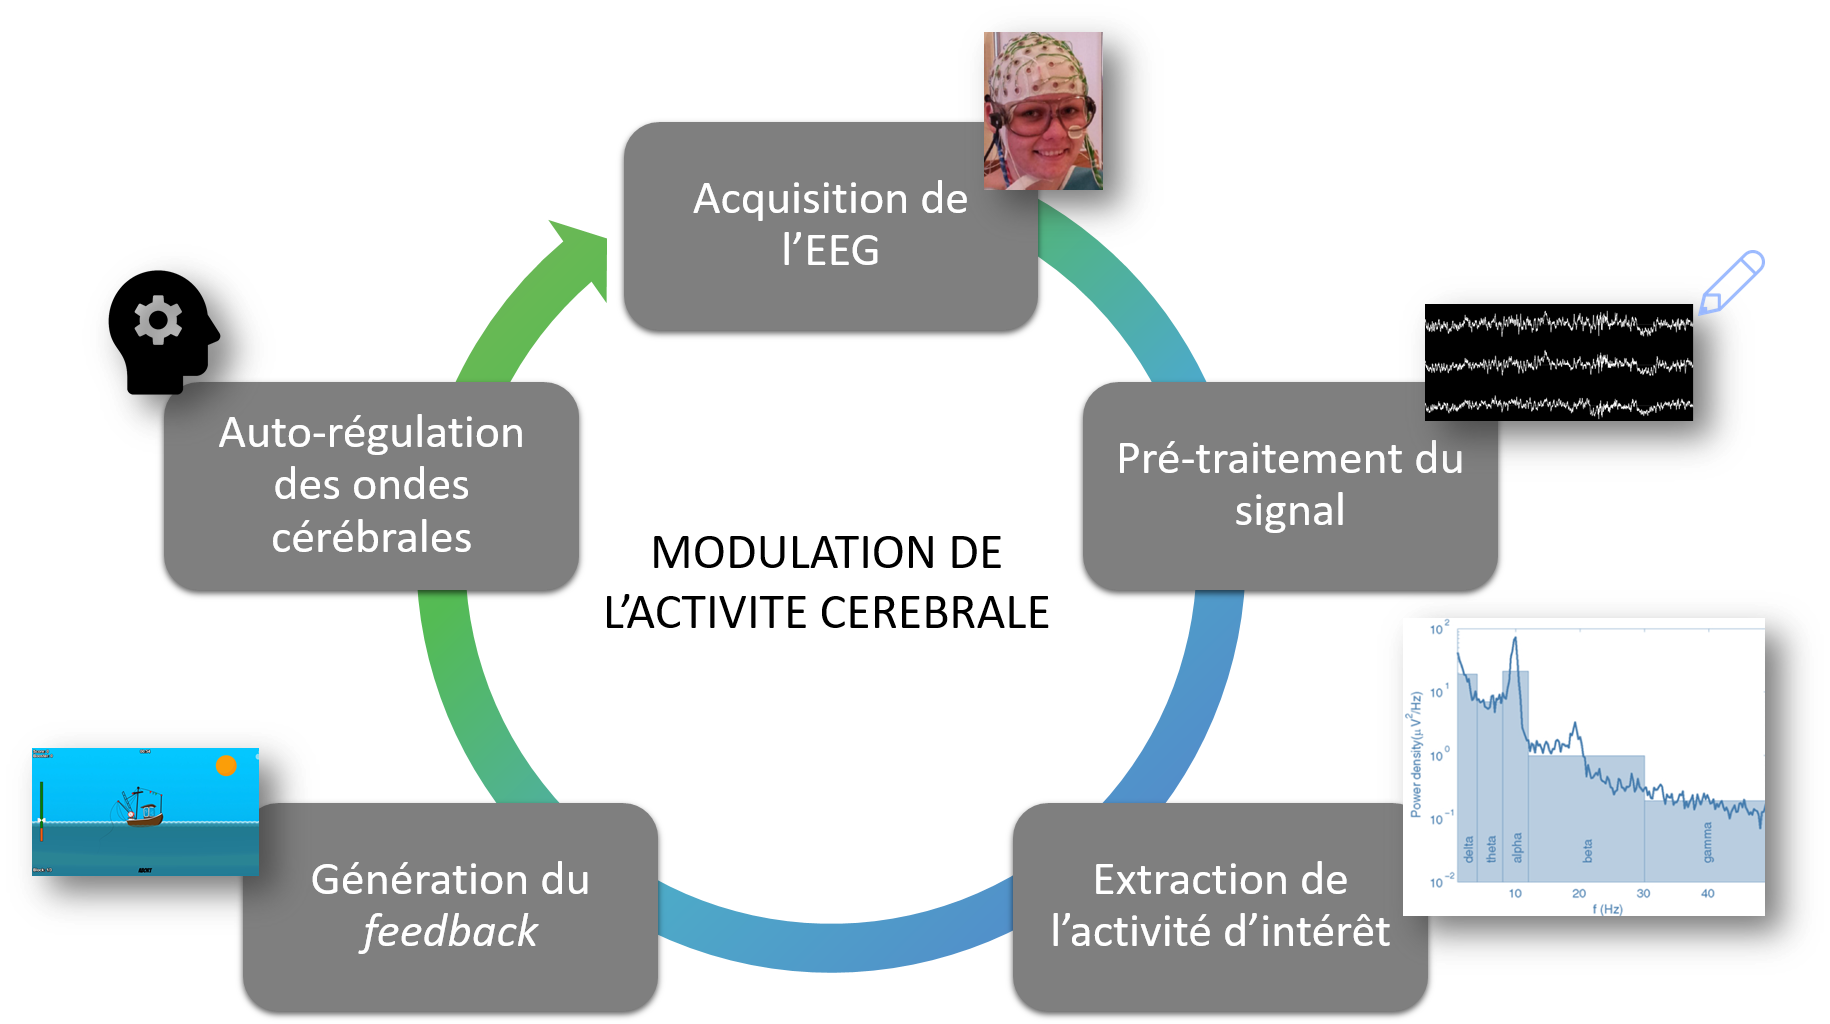
\includegraphics[width=1\linewidth]{figures/chapter-1/introduction-nfb-explication} 
  \caption{Schématisation du principe de \gls{nfb}.}
  \label{Figure:introduction_nfb_explications}
\end{figure}

\subsubsection{Déroulement d'un traitement par \gls{nfb}}

Une session de \gls{nfb} se divise généralement en plusieurs blocs d'entrainement de quelques minutes séparés par une courte période de repos.
Parmi ces blocs, certaines applications incluent 
un bloc dit de transfert durant lequel aucun retour n'est donné à l'utilisateur alors que celui-ci doit moduler son activité cérébrale \citep{Bioulac2019,
Bluschke2016, Gani2008, Strehl2006}. Cette phase de transfert a pour but de faciliter la transposition du contrôle appris durant les 
sessions de \gls{nfb} à la vie de tous les jours \citep{Arns2014}. Dans certains cas, afin d'aider cette transposition, une carte représentant l'interface du jeu sérieux est 
fournie au sujet afin qu'il puisse la regarder en modulant son activité cérébrale en dehors des sessions de \gls{nfb} \citep{Leins2007}.

L'entrainement par \gls{nfb} se compose de plusieurs sessions dont le nombre et la fréquence par semaine est variable, même lorsque le \gls{nfb} est appliqué au même trouble 
\citep{Enriquez2017}. La répétition de cet exercice de modulation cérébrale mène au phénomène de 
neuroplasticité \citep{VanDoren2017, Ros2010} qui est la capacité du cerveau de se modifier lors d'un apprentissage. Ce phénoème permet une réorganisation neuronale durable.
% parler de la dopamine ? 

\section{Les champs d'application du Neurofeedback} \label{applications_NFB}

Le \gls{nfb} peut être utilisé dans différents cas dont les principaux sont détaillés ici. Parmi ces applications, l'une d'entre elles est présentée 
plus précisément car elle est exclusivement étudiée dans la suite : le \gls{tdah} chez l'enfant.

\subsection{De nombreuses applications}

Comme détaillé précédemment, l'\gls{eeg} comporte plusieurs composantes fréquentielles dont chacune correspond à une fonction physiologique différente.
En effet, par exemple, les ondes delta sont observées lorsque le sujet est endormi, les ondes theta lorsqu'il somnole, les ondes alpha lorsqu'il est relaxé, 
les ondes beta lorsqu'il est attentif et les ondes gamma lorsqu'il est en plein processus cognitif \citep{Marzbani2016}. 

Par ailleurs, la zone sur laquelle elles sont observées est également à prendre en considération, étant donné leurs fonctions différentes comme résumées
à la Figure~\ref{Figure:introduction_cortical_areas_and_functions}.

Certains troubles se caractérisent par un surplus ou un défaut d'un rythme cérébral dans une zone donnée, comme décrit par la suite. 
Ainsi, établir un protocole de \gls{nfb} consiste à identifier ces rythmes à moduler et l'aire 
du cortex à entrainer, et à déterminer s'il faut diminuer ou augmenter la présence de ce neuromarqueur, en se basant sur la littérature 
existante \citep{Micoulaud2019}.

Les applications du \gls{nfb} peuvent donc être assez diverses, les principales sont décrites ici. 

\subsubsection{Trouble du spectre autistique}

Le trouble du spectre autistique est un trouble neurodeveloppemental qui impacte considérablement les intéractions sociales et qui est toujours présent à 
l'âge adulte. Les \gls{eeg} des enfants autistes présentent des anomalies comparés à ceux des enfants sains, notamment \citep{Coben2010, Kouijzer2010} :
\begin{itemize}
\item une activité dans les hautes fréquence de beta liée à l'anxiété,
\item une forte activité du ratio delta/theta correspondant à un déficit d'attention.
\end{itemize}
Lors de la plupart des entrainements par \gls{nfb} pour traiter le trouble du spectre autistique, il est demandé aux enfants de diminuer à la fois leur ratio 
theta/alpha et d'augmenter la production d'ondes beta dans l'aire centrale \citep{Thompson2010} et en pariétal, fontal et temporal \citep{Othmer2007}. 

\subsubsection{Epilepsie}

La recherche concernant le \gls{nfb} appliqué à l'épilepsie remonte au début de l'utilisation du \gls{nfb} avec \citet{Sterman1974}. Le protocole le plus
couramment utilisé est l'augmentation du \gls{smr} dans les zones centrales qui mène à une réduction du taux de crises d'épilepsie graves \citep{Hughes2008, Walker2010}.

\subsubsection{Gestion de la douleur}

Le \gls{nfb} a également été étudié dans la diminution de la douleur en visant directement le traitement de la perception de la douleur. Le \gls{nfb} a, par
exemple, été utilisé dans le cas de lombalgies chroniques en entrainant les ondes alpha de façon à ce qu'elles soient synchrones sur l'ensemble des aires 
cérébrales \citep{Mayaud2019}.

\subsubsection{Autres applications}

D'autres applications existent comme la diminution de l'anxiété via un protocole de diminution des ondes alpha \citep{Budzynski2009} et le traitement de la dépression
grâce à l'augmentation des ondes alpha et theta tout en diminuant les ondes beta \citep{Hurt2014}. Une application qui fait l'objet de nombreuses recherches
est le \gls{tdah}, décrite plus précisément dans la section suivante.

\subsection{Neurofeedback et \gls{tdah}} \label{nfb_and_adhd}

\subsubsection{Définition du \gls{tdah}}

% thèse pouch
% citer Lubar, voir thèse Pouch
% origine du tdah, facteurs environnementaux et/ou cliniques
% comorbidités

Le \gls{tdah} (\textit{Attention Deficit Hyperactivity Disorder} en anglais) est un trouble psychiatrique chronique qui touche environ 5\% d'enfants en âge d'aller à l'école, 
ce qui représente 2.5 millions d'enfants en Europe \citep{DSM-5}. En France, ce nombre se situe entre 3.5 et 5.6\% pour les enfants âges de 6 à 12 ans \citep{Lecendreux2011}. 
Au niveau mondial, environ 3 à 7\% des enfants d'âge scolaire sont concernés par ce trouble. Le plus forte prévalence se retouve aux Etats-Unis où 12\% des enfants et adolescents
sont diagnostiqués \gls{tdah} \citep{Collins2016}.

Ce trouble se caractérise par l'existence de trois groupes de symptômes \citep{HAS} : 
\begin{itemize}
\item le déficit attentionnel : l'enfant est dans l'incapacité de mener une tâche jusqu'au bout, il est distrait, il refuse ou évite les tâches qui demandent
une attention soutenue,
\item l'hyperactivité motrice : l'enfant ne cesse de s'agiter, il ne peut pas rester assis quand les conditions l'exigent, il fait preuve de peu d'organisation,
\item l'impulsivité : l'enfant a du mal à patienter, il a besoin d'agir et a tendance à interrompre les activités d'autrui, notamment en leur coupant la parole.
\end{itemize}
Pour certains enfants, un seul type de symptômes peut être prédominant, alors que d'autres les présentent tous de façon équivalente \citep{DSM-5}. Par ailleurs, de récentes 
études ont montré que les différents symptômes évoluent tout au long de la vie du patient \citep{CFDCAP, Epstein2013}. En effet, les symptômes du \gls{tdah}
peuvent perdurer jusqu'à l'âge adulte \citep{Faraone2006} : la prévalence des adultes \gls{tdah} augmente \citep{Chung2019}, ce qui en fait une problématique
en plein essor. Toutefois, dans la suite du manuscrit, seul le \gls{tdah} chez l'enfant est étudié. 

En plus des symptômes décrits plus haut, le \gls{tdah} impacte négativement le bien-être des enfants : ceux-ci ont, pour la plupart, une faible estime d'eux-mêmes 
\citep{Shaw2005} et de mauvais résultats scolaires \citep{Barry2002}. Ainsi, afin d'être pris en charge de façon adaptée, il est important de diagnostiquer 
le \gls{tdah} au plus tôt. 

Ce trouble est majoritairement dû à un déséquilibre de certains neurotransmitteurs du cerveau, notamment du circuit dopaminergique, 
dit circuit de la récompense \citep{Daley2010, Punja2016}.Toutefois, les causes du \gls{tdah} ne sont pas encore claires et font l'objet de discussions
dans les différentes communautés scientifiques \citep{Galera2014}. En effet, des facteurs génétiques et environnementaux entrent en jeu comme par exemple le tabagisme durant la grossesse 
et l'exposition à des pesticides durant la première année de vie \citep{Galera2014}.

En ce qui concerne le phénotype \gls{eeg} des enfants \gls{tdah}, \citet{Lubar1991} concluent que les enfants souffrant du \gls{tdah} présentent un excès d'ondes theta et un déficit d'ondes 
beta par rapport aux enfants du même âge. 
%In particular, different phenotypes of ADHD patients present with an increase in the EEG theta wave power (4–8Hz) and/or 
%a decrease of EEG beta wave power (12–32Hz) in frontal areas, or a decrease in the EEG Sensorimotor Rhythm (SMR) power (13–15Hz) in the central area (12–15)

\subsubsection{Diagnostic du \gls{tdah}}

Le diagnostic du \gls{tdah} repose dans un premier temps sur des questionnaires cliniques évaluant le comportement de l'enfant, qui peuvent ensuite être
complétés par des mesures objectives de fonctions exécutives telles que les \textit{Continuous Performance Task} \citep{Barkley1991} à l'instar du 
\textit{Test of Variables of Attention} (TOVA) \citep{Forbes1998}.

En France, le diagnostic du \gls{tdah} est établi par un spécialiste (neuropédiatre, pédopsychiatre ou neurologue en général) qui se base sur trois classifications \citep{HAS} :
\begin{itemize}
\item la CIM-10 : Classification Internationale des Maladies proposée par l'Orgnisation Mondiale de la Santé,
\item le DSM-5 : \textit{Diagnostic and Statistical Manual of Mental Disorders} dans sa 5$^{eme}$ révision de l'Association américaine de
psychiatrie,
\item la CFTMEA : Classification Française des Troubles Mentaux de l'Enfant et de l'Adolescent.
\end{itemize}

L'apparition au cours de l'enfance et le caractère persistant des symptômes s'exprimant dans différents contextes de la vie de l'individu (en privé et 
en public) sont des critères fondamentaux pour le diagnostic du \gls{tdah} \citep{HAS}. Par ailleurs, il est important de s'assurer que le comportement de
l'enfant est bien dû au \gls{tdah} et n'est pas naturel : les symptômes doivent porter préjudice au bon développement de l'enfant, aussi bien dans ses
interactions sociales qu'au cours de son apprentissage. 

Un appareil ayant pour but d'aider le diagnostic du \gls{tdah} chez l'enfant en se basant sur leur \gls{eeg} 
a été approuvé par la \citet{FDA} \citep{NebaHealth}, cependant les nouvelles études remettent en question l'utilsation de cet appareil \citep{Arns2013, 
Zhang2017}. Ainsi, des marqueurs objectifs cérébraux obtenus grâce à l'\gls{eeg} ou par \gls{fmri} ne permettraient pas d'améliorer le diagnostic pour un individu, mais
peuvent aider à distinguer différents groupes de patients \citep{Johnstone2005, Zhang2017, Clarke2011}. En effet, certains enfants \gls{tdah} 
présentent une augmentation d'ondes theta et/ou une diminution d'ondes beta dans l'aire frontale, ou une diminution du \gls{smr} dans l'aire centrale
\citep{Monastra2005, Janzen1995, Loo2018}. 

Le diagnostic du \gls{tdah} repose donc principalement sur les observations du comportement de l'enfant par leurs parents et leurs enseignants, qui souffrent de
subjectivité et pourraient mener à des diagnostics erronés \citep{Lambez2019}.

\subsubsection{Traitements existants} \label{traitements_existants}

% définition précises des approches non médicamenteuses
% discuter de l'efficacité de chaque approche
% introduire le NFB avec les études de Lubar

La HAS recommande en première intention une prise en charge non-médicamenteuse durant 3 mois à l'instar des thérapies cognitivo-comportementale \citep{HAS}. 
Ces thérapies se basent sur un système de récompenses pour encourager l'enfant à contrôler son \gls{tdah} \citep{Evans2011, Sonuga2004}.
Cependant, si ces approches se révèlent peu efficaces, un traitement médicamenteux peut être envisagé. En France seul le \gls{mph}
peut être prescrit en suivant des règles très strictes \citep{HAS}. Dans d'autres pays, d'autres molécules sont autorisées comme la lisdexamfetamine et les non-stimulantes
telles que l'atomoxetine et la guanfacine \citep{Luan2017}.

Même si le traitement médicamenteux est prescrit, la \citet{HAS} recommande de poursuivre les thérapies comportementales : un tel traitement multimodal 
est fortement conseillé dans le cadre du \gls{tdah} chez l'enfant.

Bien que très couramment utilisée,  la prise de \gls{mph} occasionne de fréquents effets secondaires,
notamment la diminution de l'appétit, le retard de croissance et des insomnies \citep{Sousa2012}. Ainsi, malgré son efficacité \citep{Taylor2014,
Storebo2015, Swanson2017}, certains parents et médecins se tournent vers des alternatives non-pharmacologiques, comme par exemple les thérapies cognitivo 
comportementales \citep{Berger2008}.

Ces thérapies se basent sur un système de récompenses pour encourager l'enfant à contrôler son \gls{tdah} \citep{Evans2011, Sonuga2004} mais se révèlent
moins efficaces que la prise de médicaments \citep{Sonuga-Barke2013}. 

Le \gls{nfb} est une autre approche non-médicamenteuse et non-invasive pour réduire les symptômes du \gls{tdah} \citep{Arns2015, Marzbani2016}.  
Plusieurs protocoles d'entrainement ont été proposés et étudiés :
\begin{itemize}
\item les protocoles basés sur les oscillations neuronales, qui visent à moduler la puissance dans des bandes fréquences données : augmentation du 
\gls{smr} \citep{Beauregard2006}, diminution du rythme theta et/ou augmentation du beta \citep{Arns2015, Kropotov2005} ; lorsque ces deux dernières 
bandes sont contrôlées simultanément on parle du protocole \gls{tbr} \citep{Lubar1976, Arns2013}, 
\item les protocoles basés sur les \textit{slow cortical potentials}, qui consistent à réguler les seuils d'excitation corticale en se concentrant sur l'activité 
générée par des siganux extérieurs \citep{Heinrich2004, Banaschewski2007},
\item les protocoles basés sur les \gls{erp} : l'amplitude de l'onde P300 peut être considérée comme un marqueur neurophysiologique spécifique de l'attention 
sélective \citep{Fouillen2017}.
\end{itemize}

Par ailleurs les protocoles peuvent également être individualisés comme décrit en \ref{principe_nfb}.

\subsubsection{Efficacité du \gls{nfb}}

La performance du \gls{nfb} dans le traitement du \gls{tdah} a fait l'objet de plusieurs études cliniques \citep{Escolano2014, Maurizio2014, Strehl2017} 
et de méta-analyses \citep{Arns2009, Micoulaud2014, Sonuga-Barke2013, Cortese2016, Catala2017, Lambez2019}. Dans ces études, l'efficacité du \gls{nfb} est 
principalement évaluée à l'aide d'échelles cliniques telles que, par exemple, l'ADHD Rating Scale \citep{Pappas2006} et la Conners \citep{Conners2008} qui sont 
des questionnaires destinés aux parents, enseignants et médecins évaluant le comportement de l'enfant. 

Avant le début de l'entrainenemt par \gls{nfb}, les évaluateurs remplissent ces questionnaires dans le but d'obtenir un score rendant compte de 
la sévérité des symptômes : généralement, plus le score est haut, plus ils sont prononcés \citep{Pappas2006, Conners2008}. Par ailleurs, certaines échelles 
permettent de calculer un score pour les composantes inattention, hyperactivité et pour les symptômes totaux \citep{Pappas2006} conduisant ainsi à une caractérisation 
plus précise du trouble. Ces questionnaires sont également remplis à l'issue de l'entrainement par les mêmes personnes afin de quantifier l'évolution 
des symptômes. 

Les évaluations des enseignants et des parents sont le plus souvent utilisées : bien que subjectives elles sont tout de même considérées comme fiables 
\citep{Mcgough2004}. Les récentes méta-analyses décrivent les parents comme non-aveugles au traitement suivi par leur enfant (ils sont dits \gls{mprox}), alors
que les enseignants sont considérés comme probablement aveugles (\gls{pblind}) et donc potentiellement insensibles à un éventuel effet placebo 
\citep{Micoulaud2014, Cortese2016}. Cependant, des études ont montré qu'enseignants et parents n'évaluent pas de la même façon les symptômes du \gls{tdah}
\citep{Sollie2013, Narad2015, Minder2018}, ce qui questionne sur la pertinence de se baser sur les évaluations \gls{pblind} pour mettre en évidence un 
effet placebo.

Alors que les parents notent une amélioration significative des symptômes après l'entrainement par \gls{nfb}, les enseignants n'observent pas des
résultats aussi favorables \citep{Arns2009, Sonuga-Barke2013, Cortese2016}, ce qui ne permet pas de conclure clairement quant à l'efficacité du \gls{nfb}.
Par ailleurs, la plupart des études sur l'efficacité du \gls{nfb} appliqué aux enfants \gls{tdah} souffent d'un faible nombre de patients inclus 
\citep{Baumeister2016, Heinrich2004} et de la difficulté, tant d'un point technique qu'éthique \citep{LaVaque2001, Birbaumer1991, Holtmann2014} de mettre en place 
un groupe contrôle qui permettrait de démontrer la présence d'un éventuel effet placebo.

En effet, dans les études d'efficacité, le \gls{nfb} peut être comparé à différents types de contrôles \citep{Arns2014} :
\begin{itemize}
\item des contrôles aux conditions semi-actives qui visent à analyser les effets non spécifiques du \gls{nfb} tels que l'importance de l'intéraction entre le sujet et le thérapeute ; 
ces contrôles ne sont pas censés avoir un effet clinique sur le \gls{tdah}. Parmi ces contrôles, on trouve les thérapies cognitives ou l'\gls{emg}-Biofeedback qui renvoie un \textit{feedback} basé
sur l'activité d'un muscle donné \citep{Bakhshayesh2011},
\item des contrôles aux conditions actives qui, eux, sont connus pour avoir un effet clinique sur les symptômes du \gls{tdah} à l'instar d'un autre protocole de \gls{nfb} \citep{Leins2007} ou
de la prise de psychostimulants \citep{Meisel2014},
\item des contrôles aux conditions placebo, le \textit{sham}-\gls{nfb}, qui sont souvent considérés comme la référence absolue en recherche. Il s'agit d'un groupe contrôle
où tout est identique, sauf le \textit{feedback} qui n'est pas calculé sur l'activité électrique du cerveau \citep{Arnold2013}. Ce type de contrôle permet 
que le sujet et tous les évaluateurs soient aveugles au traitement, évitant ainsi tout effet placebo.
\end{itemize}

Afin de confronter la performance du \gls{nfb} appliqué au \gls{tdah} aux autre traitements décrits en \ref{traitements_existants}, des histogrammes
représentant la distribution de l'efficacité de chaque traitement (quantifiée par une taille d'effet définie en \ref{es_within}) obtenue dans des études cliniques
sont tracés à la Figure~\ref{Figure:introduction-efficacy-treatments}.
Les études incluses pour le \gls{nfb} correspondent à celles sélectionnées suivant les critères d'inclusion présentés en \ref{selection_studies}, celles pour les
trois autres traitements (médicaments psychostimulants, médicaments non psychostimulants et thérapie comportementale) proviennent des plus récentes méta-analyses 
sur le sujet à disposition au moment où ce travail a été effectué \citep{Luan2017, Catala2017}.

\begin{figure}[h!]
  \centering
	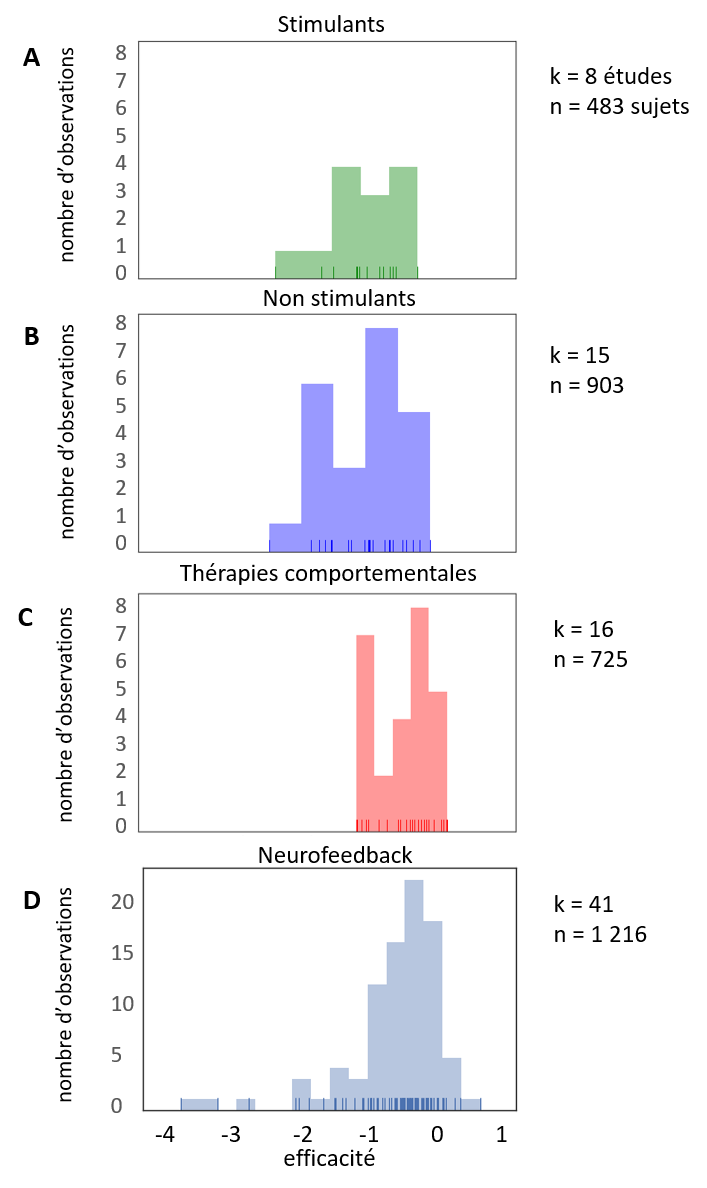
\includegraphics[width=0.5\linewidth]{figures/chapter-1/introduction-efficacy-treatments} 
  \caption{Distribution de l'efficacité des traitements couramment utilisés pour les enfants \gls{tdah} à travers les études cliniques menées : 
	psychostimulants (\textbf{A}), non psychostimulants (\textbf{B}), thérapies comportementales (\textbf{C}), \gls{nfb} (\textbf{D}). k correspond au nombre
	d'études incluses et n au nombre de sujets. 
	Une valeur d'efficacité négative est en faveur du traitement.}
  \label{Figure:introduction-efficacy-treatments}
\end{figure}

En se basant sur ces histogrammes, les traitements médicamenteux (\textbf{A} et \textbf{B}) sont les plus performants, le \gls{nfb} (\textbf{D}) présente de bons
résultats, en partie meilleurs que les thérapies comportementales (\textbf{C}). 

L'efficacité du \gls{nfb} sur le long terme a fait l'objet de quelques études, mais avec un nombre de sujets plutôt faible. Il est observé notamment
que l'entrainement par \gls{nfb} des enfants \gls{tdah} conduit à une amélioration de la mémoire de travail encore présente un an après la fin du traitement
\citep{Dobrakowski2019}. Par ailleurs, la diminution des symptômes du \gls{tdah} chez les enfants ayant effectué du \gls{nfb} reste stable 6 mois après 
l'intervention contrairement aux enfants ayant pris du méthylphénidate \citep{Gelade2018}. 

Comme tout traitement, le \gls{nfb} peut provoquer des effets secondaires notamment de la fatigue, des maux de tête, de l'anxiété, des pertubations du sommeil et de l'irritabilité qui
sont généralement observés dans  24 à 48h suivant la séance et se dissipent au-delà \citep{Hammond2007}. 


\section{Objectifs de la thèse}

Le \gls{nfb} a fait l'objet de nombreuses études pour déterminer son efficacité dans le cadre du \gls{tdah} chez l'enfant comme souligné précédemment.
Malheureusement, aucun consensus n'a encore été clairement atteint, ainsi le travail effectué au cours de cette thèse a pour but de déterminer les facteurs 
de réussite de l'entraînement par \gls{nfb} pour les enfants \gls{tdah} en se basant sur des données cliniques mais aussi physiologiques. 

Les trois sous objectifs de ce travail, chacun développé dans un chapitre, sont les suivants :
\begin{itemize}
\item étudier l'efficacité du \gls{nfb} chez les enfants \gls{tdah} à l'aide d'une méthode couramment utilisée : la méta-analyse,
\item identifier les paramètres méthodologiques et cliniques influençant la performance de ce traitement,
\item analyser la distribution d'un marqueur de l'attention (le \gls{tbr}) au sein d'une population d'enfants \gls{tdah} pour mieux cibler
l'entrainement par \gls{nfb}. 
\end{itemize}

\section{Contribution et résumé des chapitres}

Ce manuscrit est divisé en cinq parties, dont les trois centrales (les chapitres \ref{chapitre-2}, \ref{chapitre-3} et \ref{chapitre-4}) ont chacune pour but de remplir 
un des objectifs précédemment énoncés.

Avant de chercher à déterminer les facteurs de réussite de l'entrainement par \gls{nfb}, son efficacité sur les enfants \gls{tdah} est évaluée à l'aide 
d'une méthode couramment utilisée \citep{Sonuga-Barke2013, Micoulaud2014, Cortese2016} et présentée dans le chapitre \ref{chapitre-2} : la méta-analyse. 
Les résultats de ce type d'analyse ont un impact important sur la communauté scientifique : \citet{Micoulaud2016} a notamment réagi à la méta-analyse de 
\citet{Cortese2016} en discutant certains points de cette analyse. 

Ainsi, dans ce chapitre la méta-analyse de \citet{Cortese2016} qui, au moment où ce travail a été mené était la plus récente sur le sujet, est répliquée en modifiant 
les points soulignés par \citet{Micoulaud2016} afin de jauger leur impact sur les conclusions émises dans la méta-analyse. Ensuite, étant donné que de nouvelles études 
satisfaisant les critères d'inclusion établis par \citet{Cortese2016} sont disponibles, cette méta-analyse est mise à jour : en plus des 13 études originellement incluses, 3
sont ajoutées, ce qui apporte une plus grande puissance statistique aux résultats. La réplication et la mise à jour sont effectuées, non pas avec les logiciels 
habituellement utilisés tels que Revman \citep{Revman}, mais à l'aide d'un package Python développé pour cette occasion et disponible en ligne afin de favoriser 
la réplication et/ou la mise à jour de ce travail. 

La réplication de la méta-analyse conduisant aux mêmes résultats que \citet{Cortese2016}, les choix discutés par \citet{Micoulaud2016} n'ont pas un impact assez
important pour changer ses conclusions : le \gls{nfb} est jugé efficace par les parents alors que les enseignants, considérés comme \gls{pblind}, ne notent aucune
amélioration significative. Par ailleurs, la mise à jour confirme les résultats qui semblent commencer à se stabiliser pour les évaluations des parents.

Ce chapitre a été l'occasion de mener une revue de littérature des études d'efficacité sur le \gls{nfb} appliqué aux enfants \gls{tdah} 
qui a permis de mettre en évidence la forte hétérogénéité d'un point de vue clinique et méthodologique de ces études. 

Alors que la fiabilité des résultats des méta-analyses souffre de ces différences qui pourraient, par ailleurs, expliquer l'absence de consensus quant 
à l'efficacité du \gls{nfb} \citep{Alkoby2017}, une analyse en tirant avantage est implémentée : la \gls{saob} décrite dans le chapitre \ref{saob}. 

Les facteurs méthodologiques et/ou cliniques fortement variables entre les études tels que, par exemple, la durée du traitement, le nombre de sessions et le type 
de protocole de \gls{nfb} suivi, sont extraits de 33 études d'efficacité sur le \gls{nfb} appliqué aux enfants \gls{tdah}, dans le but de déterminer lesquels 
ont un impact sur l'efficacité du \gls{nfb}. Pour ce faire, trois méthodes multivariées sont utilisées : la \gls{wls}, le \gls{lasso} et le \gls{dt}. 

La \gls{saob} identifie trois facteurs qui semblent avoir un impact sur l'efficacité du \gls{nfb} : tout d'abord, utiliser un matériel d'acquisition de bonne 
qualité conduirait à de meilleurs résultats, ensuite un traitement intensif semblerait préférable, et enfin les évaluations des enseignants seraient plus
sévères quant à l'amélioration du traitement. 

La personnalisation des protocoles de \gls{nfb} est un facteur dont il aurait été intéressant d'étudier l'impact sur l'efficacité du \gls{nfb}.  
Cependant, faute d'un nombre suffisant d'études ayant recours à la personnalisation, ce facteur n'a pas pu être étudié dans la \gls{saob}. C'est pourquoi
la pertinence d'une personnalisation est étudiée dans le chapitre \ref{chapitre-4} grâce à l'analyse de la distribution d'un marqueur de l'attention : le \gls{tbr} pour
lequel de précédentes études ont montré qu'il serait variable au sein de la population \gls{tdah} \citep{Zhang2017, Arns2013, Clarke2001}.

Le \gls{tbr} est extrait de 363 \gls{eeg} d'enfants \gls{tdah} qui vont être partitionnés grâce à trois méthodes : le \gls{bgmm}, le partitionnement
hiérarchique basé sur la distance de Ward et le \gls{dbscan}. Si la distribution est trouvée bimodale par ces trois méthodes, les seuils calculés par chaque méthode,
sont comparés, notamment grâce à une courbe \gls{roc} obtenue sur
les résultats du \gls{bgmm} afin de déterminer celui sur lequel il faudrait se baser pour attribuer le protocole de \gls{nfb}.

Les trois méthodes s'accordent sur le fait que la distribution des \gls{tbr} est bimodale, ce qui indique qu'il existe en effet deux groupes d'enfants
\gls{tdah} : l'un présentant des \gls{tbr} plutôt faibles et l'autre avec des \gls{tbr} élevés. Ainsi, personnaliser le protocole de \gls{nfb} en 
fonction de la valeur de \gls{tbr} semblerait pertinent et après comparaison des seuils \gls{tbr} obtenus, celui de 4.1 apporte le plus d'équilibre entre 
un faible taux de faux positifs et un taux de vrais positifs élevé.  

\section{Liste des publications}

Le travail décrit dans ce manuscrit a donné lieu aux publications avec comité de lecture suivantes :

\begin{description}
\item \citet{Bussalb2019tbr} : A. Bussalb, S. Collin, Q. Barthélemy, D. Ojeda, S. Bioulac, H. Blasco-Fontecilla,
D. Brandeis, D. P. Ouakil, T. Ros, and L. Mayaud. Is there a cluster of high
theta-beta ratio patients in attention deficit hyperactivity disorder ? \textit{Clinical Neurophysiology}, 2019a.
\item \citet{Bussalb2019clinical} : A. Bussalb, M. Congedo, Q. Barthélemy, D. Ojeda, E. Acquaviva, R. Delorme,
and L. Mayaud. Clinical and experimental factors influencing the efficacy of
neurofeedback in ADHD: a meta-analysis. \textit{Frontiers in psychiatry}, 10 :35, 2019b.
\end{description}

Une partie des travaux de \citet{Bussalb2019clinical} ont fait l'objet d'une communication orale :

\noindent A. Bussalb, M. Congedo, R. Delorme, E. Acquaviva, Q. Barthelemy, D. Ojeda, J.A. Micoulaud-Franchi, L. Mayaud. Neurofeedback 
appliqué aux enfants TDAH : quels facteurs influencent son efficacité ? 6ème Congrès de la SOFTAL, mai 2018. 


% définir epoque

\newpage
\chapter{Evaluation de l'efficacité du Neurofeedback par la méta-analyse} \label{chapitre-2}

\section*{Introduction}
Les méta-analyses ont pour but de combiner les données de plusieurs études visant à démontrer l'efficacité d'un traitement. Cette méthode est
particulièrement intéressante lorsque les études comportent un faible nombre de sujets ou que les résultats des études se contredisent, 
comme c'est notamment le cas pour le \gls{nfb} appliqué aux enfants \gls{tdah}, qui est l'un des principaux usages du \gls{nfb}. 

Les différentes étapes à suivre pour réaliser une méta-analyse sont détaillées précisément dans ce chapitre.
Ces étapes sont ensuite appliquées à la réplication et à la mise à jour d'une récente méta-analyse sur l'efficacité du \gls{nfb} appliqué aux enfants 
souffrant de \gls{tdah} :
celle de \citet{Cortese2016} dont certains résultats ont été débattus par la communauté scientifique \citep{Micoulaud2016}. Ainsi, cette analyse a pour but
de relever l'éventuel impact de certains choix méthodologiques de \citet{Cortese2016} sur ses conclusions quant à l'efficacité du \gls{nfb} et de mettre à jour
ces résultats en incluant de nouvelles études. 

A travers le travail présenté ici, la performance du \gls{nfb} sur les enfants \gls{tdah} est alors évaluée et la revue de littérature
qui a été menée a permis de se familiariser avec les études sur l'efficacité de ce traitement et d'en noter les éventuelles faiblesses.

\newpage

\section{Principe d'une méta-analyse} \label{methods}

Les différentes étapes pour réaliser une méta-analyse sont décrites dans cette partie et résumées à la Figure~\ref{Figure:pipeline_meta_analyse}. 
Bien qu'il existe des logiciels permettant de réaliser une méta-analyse, ces étapes ont été implémentées en Python par souci de transparence et de reproductibilité. 
En effet, les logiciels généralement employés proposent une interface graphique où les formules mathématiques utilisées ne sont pas énoncées clairement. Le code source de ce package 
Python est disponible sur un dépôt GitHub \citep{Bussalb2019clinical} avec sa documentation associée générée par Sphinx (version 1.5.6.).

\subsection{Buts d'une méta-analyse}

Les méta-analyses rassemblent les résultats de plusieurs études, satisfaisant des critères d'inclusion préalablement établis, dans le but d'analyser
sur un plus grand nombre de sujets provenant de populations différentes, l'efficacité d'un traitement. 

\begin{figure}[h!]
  \centering
	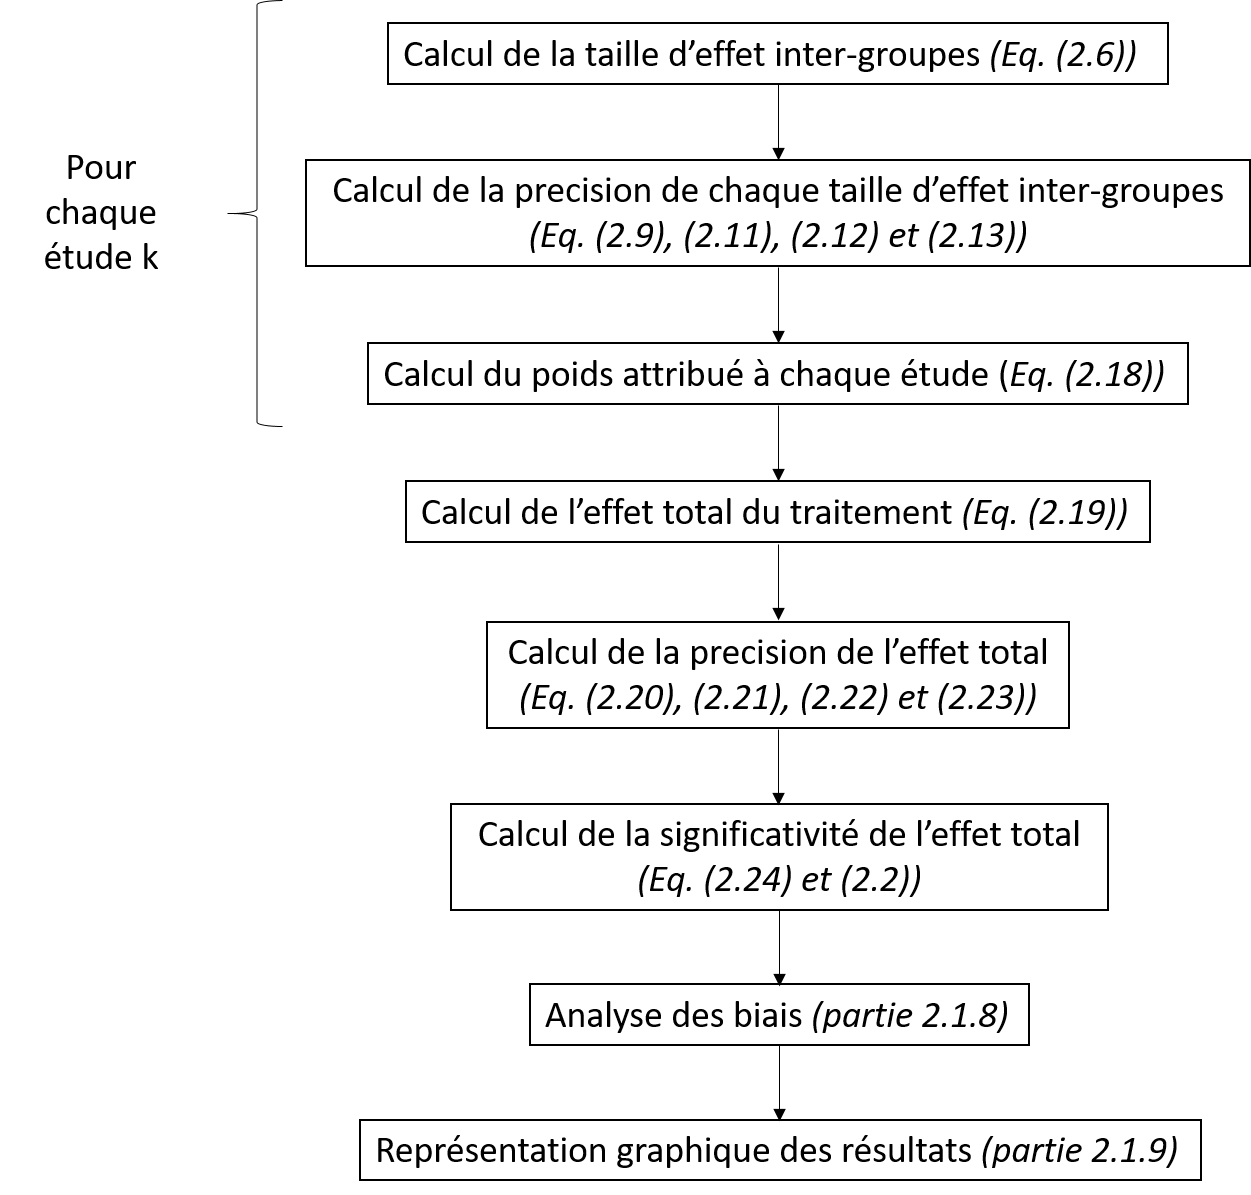
\includegraphics[width=1.0\linewidth]{figures/chapter-2/pipeline-perform-meta-analysis} 
  \caption[Résumé des étapes d'une méta-analyse.]{Résumé des étapes à suivre pour effectuer une méta-analyse dans le cadre d'un modèle à effets aléatoires.}
  \label{Figure:pipeline_meta_analyse}
\end{figure}

Alors qu'avant les années 1990 les revues narratives (\textit{narrative reviews} en anglais) étaient le plus couramment utilisées pour cette tâche, elles ont 
perdu leur popularité au profit des méta-analyses. En effet, les revues narratives souffrent de la subjectivité des auteurs qui choisissent notamment le poids 
à donner à telle ou telle étude : alors que certains
vont donner plus d'importance aux études incluant de nombreux sujets, d'autres vont favoriser celles qu'ils jugent de bonne qualité. La méta-analyse permet 
de réduire cette subjectivité en utilisant par exemple des critères mathématiques définis à l'avance pour calculer le poids à attribuer à chaque étude incluse
\citep[Chapitre~1]{Borenstein2009}. 

Par ailleurs, des recommandations précises quant à la conduite d'une méta-analyse existent \citep{Moher2009, Cochrane}. Ces recommandations
appellent notamment à apporter un soin particulier à la sélection des études qui doivent répondre à des critères d'inclusion fixés 
\textit{a priori} et à évaluer le risque de biais intra et inter-études, comme le biais de publication \citep{Higgins2011}. Ce biais consiste, 
pour un chercheur, à avoir tendance à publier des expériences présentant des résultats statistiquement significatifs.  

Réaliser une méta-analyse permet de confronter les résultats de toute étude incluse à ceux des autres études intégrées dans l'analyse.
L'efficacité du traitement observée pour chaque étude est mesurée à l'aide d'une valeur appelée taille 
d'effet (ou \gls{es} en anglais) présentée en \ref{definition_es} qui est, le plus souvent, standardisée du fait du regroupement de 
populations et de mesures relativement hétérogènes \citep{Cortese2016}.

\subsection{Choix du modèle} \label{model_choice}

La première étape consiste à choisir le modèle statistique de la méta-analyse. La plupart des méta-analyses sont basées sur l'un des deux modèles 
suivants qui reposent sur des hypothèses scientifiques différentes \citep[Chapitre~10]{Borenstein2009} :
\begin{itemize}
\item le modèle à effet fixe (\textit{fixed-effect model} en anglais),
\item le modèle à effets aléatoires (\textit{random-effects model} en anglais).
\end{itemize}

Dans le cas du modèle à effet fixe, il est supposé qu'il existe un \gls{es} réel (\textit{true} \gls{es} en anglais), c'est à dire l'\gls{es} qui serait
observé avec un nombre de sujets infiniment grand, qui serait le même pour l'ensemble des études incluses dans la méta-analyse. Les différences entre
les \gls{es} observés pour chaque étude sont dues à des erreurs d'échantillonnage. Au contraire, dans le cas du modèle à effets aléatoires, 
l'\gls{es} réel peut varier entre les études. Cette variabilité s'explique non seulement par des erreurs d'échantillonnage, mais aussi par 
les différentes conceptions des études et/ou par les différences entre les sujets inclus.

Les \gls{es} obtenus pour chaque étude sont moyennés pour mener à un \gls{est} (\textit{summary effect} en anglais dont le calcul est
décrit en \ref{compute_summary_effect}) sur lequel une hypothèse nulle est testée, qui diffère selon le modèle choisi :
\begin{itemize}
\item pour le modèle à effet fixe : 
\textit{$H_{0}$ : le traitement n'a auncun effet dans chaque étude},
\item pour le modèle à effets aléatoires : 
\textit{$H_{0}$ : l'effet moyen du traitement est nul}.
\end{itemize}

Le modèle à effets aléatoires est souvent plus approprié du fait de la variabilité des études. En effet, même si les études incluses dans la méta-analyse 
répondent toutes aux critères d'inclusion fixés au préalable, rien ne peut généralement permettre de supposer que ces études sont identiques et qu'elles 
partagent donc toutes le même \gls{es} réel. Le modèle à effet fixe est ainsi rarement utilisé, on peut cependant y avoir recours lorsque le nombre d'études incluses 
est très petit. En effet, dans le cas du modèle à effet fixe, les poids associés à chaque étude sont moins équilibrés : les études incluant un grand nombre de 
sujets se voient attribuer un poids plus important que dans le cas du modèle à effets aléatoires, et les études aux petits échantillons un plus faible poids.

Au sein du domaine du \gls{nfb} appliqué aux enfants \gls{tdah}, les méta-analyses suivent le modèle à effets aléatoires 
\citep{Cortese2016, Micoulaud2014}. Ainsi, étant donné l'hétérogénéité des populations étudiées et des critères d'évaluation, et pour être en accord avec
la littérature existante, c'est le modèle à effets aléatoires qui est utilisé par la suite.

\subsection{Calcul de la taille d'effet} \label{definition_es}

Une fois le modèle choisi, l'étape suivante est de quantifier l'efficacité de chaque étude incluse dans la méta-analyse en calculant son \gls{es}. 
Il existe différents \gls{es} \citep[Chapitre~3]{Borenstein2009} :
\begin{itemize}
\item \gls{es} basés sur des \emph{moyennes} :
\begin{itemize}
    \item la différence moyenne non standardisée (\textit{unstandardized mean difference} en anglais), D :
		    \begin{equation}
        \label{eq:metareview_unstandardized_mean_difference}
        \text{D} = \mu_{1} - \mu_{1},
        \end{equation} 
		avec $\mu_{1}$ et $\mu_{2}$ les moyennes de deux groupes indépendants, ou du même groupe à pré- et à post-test,
    \item la différence moyenne standardisée (\textit{standardized mean difference} en anglais), d :
		    \begin{equation}
        \label{eq:metareview_standardized_mean_difference}
        \text{d} = \frac{\mu_{1} - \mu_{2}}{\sqrt{\frac{(n_1 - 1)\sigma_1^2 + (n_2 - 1)\sigma_2^2} {n_1 + n_2 - 2}}},
        \end{equation} 
		avec $n_{1}$ et $n_{2}$ le nombre de sujets dans les groupes 1 et 2, et $\sigma_{1}$ et $\sigma_{2}$ les écarts-types des deux groupes. Le dénominateur
		correspond à l'écart type intra-groupe calculé à travers les deux groupes.
\end{itemize}
\item \gls{es} basés sur des \emph{données binaires} :
\begin{itemize}
    \item le taux de risque (\textit{risk ratio} en anglais), RR :
				\begin{equation}
        \label{eq:metareview_risk_ratio}
        \text{RR} = \frac{ \text{A} / n_1 } { \text{C} / n_2 },
        \end{equation} 
		avec A et C le nombre d'évènements observés (par exemple présence d'un effet secondaire) respectivement dans les groupes 1 et 2,
    \item le taux de chance (\textit{odds ratio} en anglais), OR :
				\begin{equation}
        \label{eq:metareview_odds_ratio}
        \text{OR} = \frac{ \text{AD} } { \text{BC} },
        \end{equation} 		
		avec D et B le nombre de non-évènements observés (par exemple absence d'un effet secondaire) respectivement dans les groupes 2 et 1,
		\item la différence de risque (\textit{risk difference} en anglais), RD :
				\begin{equation}
        \label{eq:metareview_risk_difference}
        \text{RD} = \frac{ \text{A} } { n_1 } - \frac{ \text{C} } { n_2 }.
        \end{equation}
\end{itemize}
\end{itemize}

Etant donné que les données que nous allons utiliser pour la réplication et la mise à jour de \citet{Cortese2016} sont les moyennes des 
scores cliniques obtenus par les sujets sur des échelles évaluant les symptômes du \gls{tdah} avant le traitement (pré-test) et 
après le traitement (post-test) et leur écart-type, nous nous concentrons sur 
les \gls{es} basés sur des moyennes. Par ailleurs, les échelles cliniques variant 
d'une étude à l'autre, les moyennes et les écarts-types ne sont pas comparables : il faut donc standardiser l'\gls{es}. 
Ainsi, nous allons utiliser la différence moyenne standardisée \citep{Cortese2016, Micoulaud2014}.

Enfin, lorsqu'un groupe contrôle est disponible, on peut calculer l'\gls{es}-inter-groupes (\textit{between}-\gls{es} en anglais) comme défini par \citet{Morris2008}.
Cet \gls{es} est utilisé par \citet{Cortese2016} et \citet{Micoulaud2014} et implémenté dans \citet{Bussalb2019clinical} :
\begin{equation}
\label{eq:metareview_effect_size_between}
\text{ES-inter-groupes} = c_p \left(\frac{(M_{\text{post},T} - M_{\text{pré},T}) - (M_{\text{post},C} - M_{\text{pré},C}) }{\sigma_{\text{pré}}} \right).
\end{equation} 

L'\gls{es}-inter-groupes est équivalent au $Z$-score d'une distribution normale qui est une mesure de combien d'écarts-types un score brut est au-dessus ou en-dessous
de la moyenne d'une population. 

L'\gls{es}-inter-groupes correspond à la différence entre la moyenne à post-test et à pré-test 
dans le groupe qui reçoit le traitement ($M_{\text{post},T}$, $M_{\text{pré},T}$) moins la différence entre la moyenne du score à post-test et à pré-test 
dans le groupe contrôle ($M_{\text{post},C}$, $M_{\text{pré},C}$), divisée par la \textit{pooled standard deviation} à pré-test ($\sigma_{\text{pré}}$) :
\begin{equation}
\label{eq:stats_metareview_std_pre}
\sigma_{\text{pré}} = \sqrt{\frac{(n_T - 1)\sigma_{\text{pré}, T}^2 + (n_C - 1)\sigma_{\text{pré}, C}^2} {n_T + n_C - 2}},
\end{equation}
où $\sigma_{\text{pré},G}$ correspond à l'écart-type du groupe $G$ à pré-test et $n_G$ indique le nombre de sujets ayant suivi l'intégralité 
du traitement dans chaque groupe.

La normalisation de l'\gls{es}-inter-groupes (équation Eq.~(\ref{eq:metareview_effect_size_between})) à l'aide de $\sigma_{\text{pré}}$ 
(équation Eq.~(\ref{eq:stats_metareview_std_pre})) se fait seulement avec les données obtenues en pré-test pour ne pas y inclure la variabilité 
induite par le traitement.

Il s'avère que l'\gls{es}-inter-groupes présente un léger biais qui tend à sous-estimer la valeur absolue de la différence moyenne standardisée de la population
lorsque les études incluent peu de sujets. Cette valeur est obtenue en calculant la différence entre les vraies moyennes de la population de chaque groupe divisée 
par l'erreur type de la vraie population qui est supposée être identique pour les deux groupes \citep[Chapitre~4]{Borenstein2009}. Ce biais peut être supprimé 
grâce à un facteur de correction $c_p$ qui est utilisé pour les petites études (c'est à dire pour lesquelles $n_T + n_C - 2 < 10$) : 
\begin{equation}
\label{eq:metareview_correction_factor}
c_p =  1 - \frac{3} {4(n_T + n_C - 2) - 1},
\end{equation} 
avec $n_T + n_C - 2$ qui correspond au dégré de liberté utilisé pour le calcul de $\sigma_{\text{pré}}$ à l'équation Eq.~(\ref{eq:stats_metareview_std_pre}).

Plus la valeur absolue de l'\gls{es}-inter-groupes est élevée, plus l'efficacité du traitement est importante.

\subsection{Calcul de la fiabilité de chaque taille d'effet}

Le terme précision englobe trois valeurs statistiques liées les unes aux autres : la variance, l'\gls{et} (à ne pas confondre avec
l'écart type), et l'intervalle de confiance.
Ces trois facteurs de précision définissent un intervalle de valeurs probables pour l'\gls{es} réel. 

Tout d'abord, la variance de chaque \gls{es}-inter-groupes est calculée \citep{Morris2008}:
\begin{equation}
\label{eq:metareview_variance_effect_size_between}
\sigma^2(\text{ES}) = c_p^2 \left(
    \frac{n_T + n_C - 2} {n_T + n_C - 4} 
\right ) \left ( 
		\frac{2(1-r)(n_T + n_C)} {n_Tn_C} + \text{ES}^2 
\right) - \text{ES}^2,
\end{equation}
où \gls{es} désigne l'\gls{es}-inter-groupes et $r$ la corrélation de Pearson groupée intra-groupes \citep{James2013} :
\begin{equation}
\label{eq:metareview_within_group_pearson_correlation}
r = \frac{ \sum_{i=1}^{n} (\text{s}_{\text{pré},i} - \mu_{\text{pré}})(\text{s}_{\text{post},i} - \mu_{\text{post}}) } { \sqrt{ \sum_{i=1}^{n} (\text{s}_{\text{pré},i} - 
\mu_{\text{pré}})^2} \sqrt{\sum_{i=1}^{n} (\text{s}_{\text{post},i} - \mu_{\text{post}})^2} }, 
\end{equation}
où $n$ est le nombre de patients inclus dans une étude, $\text{s}_{\text{pré},i}$, $\text{s}_{\text{post},i}$ les valeurs de scores cliniques pour le sujet $i$ 
respectivement à pré- et post-test, et $\mu_{\text{pre}}$, $\mu_{\text{post}}$ les scores moyens calculés sur tous les sujets. 
Il s'agit d'une mesure de corrélation linéaire entre deux variables : une valeur de 1 signifie une corrélation positive entre ces variables,
une valeur de -1 une corrélation négative, et une valeur de 0 une absence de corrélation linéaire. Ainsi, si le traitement n'a aucun effet, 
que l'état des sujets n'évolue pas naturellement, et en l'absence de bruit, $r$ sera égal à 1. On peut en déduire alors qu'une étude 
composée d'enfants plus jeunes qui sont davantage susceptibles de changer naturellement va présenter une valeur de $r$ plus faible, il en va 
de même si le traitement est efficace. Enfin la présence de bruit va également avoir un impact sur cette valeur. Par conséquent, une valeur 
de $r$ doit être calculée pour chaque étude.

Dans notre cas, cette corrélation étant inconnue et les données brutes n'étant pas disponibles pour la majorité des études cliniques, nous approximons la valeur 
de $r$ en accord avec \citet{Balk2012}, qui a trouvé qu'une valeur de 0.5 conduit à des résultats proches de ceux obtenus avec la véritable
valeur de la corrélation.

Une fois la variance obtenue, il est aisé de calculer l'\gls{et} (\textit{standard error} en anglais) de l'\gls{es}-inter-groupes \citep[Chapitre~8]{Borenstein2009} :
\begin{equation}
\label{eq:metareview_standard_error_effect_size_between}
\text{ET} = \sqrt{\sigma^2(\text{ES})} = \sigma(\text{ES}),
\end{equation}
où \gls{es} désigne l'\gls{es}-inter-groupes. Alors que la variance est intéressante pour les calculs statistiques, l'\gls{et} est quant à elle 
un index plus aisé à comprendre car elle est sur la même échelle que l'\gls{es}.

Enfin, si on suppose que l'\gls{es}-inter-groupes suit une distribution normale, son intervalle de confiance à 95\% peut être calculé \citep[Chapitre~8]{Borenstein2009} :
\begin{equation}
\label{eq:metareview_es_between_confidence_interval_95_lower_bound}
\text{LL} = \text{ES-inter-groupes} - 1.96 * \text{ET},
\end{equation}
et 
\begin{equation}
\label{eq:metareview_es_between_confidence_interval_95_upper_bound}
\text{UL} = \text{ES-inter-groupes} + 1.96 * \text{ET},
\end{equation}
où LL correspond à la limite inférieure de l'intervalle et UL à la limite supérieure. La valeur de 1.96 correspond au $Z$-score d'une distribution 
normale standard pour un intervalle de confiance à 95\%. La probabilité de trouver dans cet intervalle
la vraie valeur de l'\gls{es}-inter-groupes de la population est de 95\%.

La précision est affectée, dans une large mesure, par le nombre de sujets inclus dans l'étude : les échantillons plus grands mènent à des
variances plus faibles et donc à des estimations d'\gls{es}-inter-groupes plus précises \citep[Chapitre~8]{Borenstein2009}, c'est pourquoi un plus grand 
poids leur est attribué dans la méta-analyse comme détaillé par la suite.

\subsection{Calcul de la taille d'effet totale du traitement} \label{compute_summary_effect}

Afin d'obtenir l'estimation la plus précise possible de l'effet du traitement sur la population, une moyenne pondérée des \gls{es}-inter-groupes 
des études incluses est calculée.

Si le modèle à effet fixe est choisi, le poids $w_{\text{fixe},k}$ assigné à chaque étude $k$ correspond à l'inverse de la variance de son 
\gls{es}-inter-groupes ($\sigma^2(\text{ES})$, la variance intra-étude) \citep[Chapitre~12]{Borenstein2009} :
\begin{equation}
\label{eq:metareview_weight_fixed_study}
w_{\text{fixe},k} = \frac{1}{\sigma^2(\text{ES}_k)}.
\end{equation} 

Cette étape a pour but de minimiser l'importance des études avec une large variabilité intra-étude.

Dans notre cas nous employons le modèle à effets aléatoires, qui inclut également la variance inter-études $\tau^2$ conduisant à des 
poids $w_{\text{aléatoires},k}$, simplement notés $w_k$ par la suite, associés aux études différents.
Toutefois, afin d'obtenir les poids $w_k$, il est nécessaire de calculer d'abord les $w_{\text{fixe},k}$ grâce à l'équation 
Eq.~(\ref{eq:metareview_weight_fixed_study}).

Calculer la variance inter-études se fait en trois étapes décrites par les équations Eq.~(\ref{eq:metareview_Q}), Eq.~(\ref{eq:metareview_C}) 
et Eq.~(\ref{eq:metareview_Tau}) \citep[Chapitre~12]{Borenstein2009} :
\begin{equation}
\label{eq:metareview_Q}
Q = \sum_{k=1}^{K} w_{\text{fixe},k} * \text{ES}_k^2,
\end{equation}
\begin{equation}
\label{eq:metareview_C}
C = \sum_{k=1}^{K} w_{\text{fixe},k} - \frac{ \sum_{k=1}^{K} (w_{\text{fixe},k})^2 } { \sum_{k=1}^{K} w_{\text{fixe},k} },
\end{equation}
avec $K$ le nombre total d'études incluses, et :
\begin{equation}
\label{eq:metareview_Tau}
\tau^2 = \frac{Q - \text{df}}{C},
\end{equation}
avec $\text{df} = K - 1$ le degré de liberté.

Le modèle à effets aléatoires prenant en compte les différences entre les études, les poids sont égaux à l'inverse de la somme entre la variance intra-étude
$\sigma^2(\text{ES}_k)$ et la variance inter-études $\tau^2$ \citep[Chapitre~12]{Borenstein2009} :
\begin{equation}
\label{eq:metareview_weight_study}
w_k = \frac{1}{\sigma^2(\text{ES}_k) + \tau^2}.
\end{equation} 

Enfin, la moyenne pondérée des $K$ \gls{es}-inter-groupes est calculée pour obtenir l'\gls{est} comme décrit dans l'équation
Eq.~(\ref{eq:metareview_summary_effect}) \citep[Chapitre~12]{Borenstein2009}:
\begin{equation}
\label{eq:metareview_summary_effect}
\text{EST} = \frac{\sum_{k=1}^{K} w_k * \text{ES}_k} {\sum_{k=1}^{K} w_k}.
\end{equation} 

\subsection{Calcul de la fiabilité de la taille d'effet totale}

Une fois l'\gls{est} obtenu, on peut calculer ses trois valeurs de précision \citep[Chapitre~12]{Borenstein2009}. Tout d'abord, sa variance $\sigma^2(\text{EST})$ :  
\begin{equation}
\label{eq:metareview_variance_summary_effect}
\sigma^2(\text{EST}) = \frac{1} {\sum_{k=1}^{K} w_k},
\end{equation} 
puis son \gls{et} ET(EST) :
\begin{equation}
\label{eq:metareview_standard_error_effect}
\text{ET(EST)} = \sqrt{\sigma^2(\text{EST})} = \sigma(\text{EST}),
\end{equation} 
et enfin son intervalle de confiance à 95\% : 
\begin{equation}
\label{eq:metareview_confidence_interval_summary_effect_lower_bound}
\text{LL(EST)} = \text{EST} - 1.96 * \text{ET(EST)},
\end{equation}
et 
\begin{equation}
\label{eq:metareview_confidence_interval_summary_effect_upper_bound}
\text{UL(EST)} = \text{EST} + 1.96 * \text{ET(EST)},
\end{equation}
avec LL la limite inférieure de cet intervalle de confiance et UL sa limite supérieure.

\subsection{Calcul de la significativité statistique de la taille d'effet totale}

Une $Z$-value est calculée pour tester l'hypothèse nulle pour le modèle à effets aléatoires énoncée en \ref{model_choice} \citep[Chapitre~12]{Borenstein2009} :
\begin{equation}
\label{eq:metareview_confidence_interval_summary_effect_z_value}
Z = \frac{\text{EST}} {\text{ET(EST)}}.
\end{equation}

Pour un test bilatéral (utilisé par \citet{Micoulaud2014, Cortese2016}), la $p$-value est ensuite calculée avec \citep[Chapitre~12]{Borenstein2009} :
\begin{equation}
\label{eq:metareview_confidence_interval_summary_effect_p_value}
p = 2(1 - \Phi(\abs{Z})),
\end{equation} 
où $\Phi$ est la fonction de distribution cumulative de la loi normale standardisée (\textit{i.e.} centrée et normée).

Si la $p$-value obtenue est inférieure à 0.05, alors il y a une différence statistiquement significative entre l'efficacité du traitement étudié 
et celle du groupe contrôle.

D'autres valeurs peuvent ensuite être calculées pour compléter l'analyse, comme par exemple $I^2$ qui estime 
l'hétérogénéité des \gls{es}-inter-groupes \citep[Chapitre~16]{Borenstein2009}. 

\subsection{Analyse des biais}

Les résultats d'une méta-analyse peuvent être impactés par des biais, comme par exemple un biais de publication qui consiste en la tendance qu'ont les auteurs 
d'études scientifiques de plutôt publier des résultats statistiquement significatifs et en faveur de ce qu'ils veulent démontrer. De plus,
d'autres facteurs peuvent influencer les résultats de la méta-analyse : une faible qualité méthodologique conduisant à des effets faussement gonflés
dans les petites études, l'hétérogénéité des \gls{es} selon la taille des études, et le hasard \citep{Sterne2011}.

L'analyse visuelle de la symétrie d'un \textit{funnel plot} est une méthode couramment utilisée pour détecter un éventuel biais de publication et 
l'influence des facteurs cités précédemment \citep{Sterne2011}.

Il s'agit d'un nuage de points de la précision de chaque \gls{es}-inter-groupes en fonction des \gls{es}-inter-groupes. L'\gls{et} est couramment 
utilisée comme estimation de la précision et de la taille d'une étude et est placée sur un axe des abscisses inversé de façon à ce que les plus grandes études 
soient au sommet et que les plus petites se retrouvent 
dispersées en bas. En l'absence de biais et d'hétérogénéité entre les études, la répartition des points est seulement due à la variabilité de la taille des études : 
le graphique est symétrique. Le triangle centré sur l'\gls{est}, obtenu avec un modèle à effet fixe et s'étendant de 1.96 \gls{et} de chaque côté, 
inclut 95\% des études s'il n'y a pas de biais et si l'hypothèse du modèle à effet fixe est valide.

Déterminer l'asymétrie d'un \textit{funnel plot} peut se faire visuellement mais aussi mathématiquement en utilisant, par exemple, le test d'\citet{Egger1997}. 
Il s'agit de régresser les \gls{es}-inter-groupes divisés par leur \gls{et} sur l'inverse des \gls{et}. Si l'ordonnée à l'origine (\textit{intercept} en anglais) diffère significativement de 
zéro (seuil de significativité statistique à 5\%), alors le \textit{funnel plot} est asymétrique.

\subsection{Représentation graphique des résultats d'une méta-analyse}

Afin de faciliter la lecture des résultats d'une méta-analyse, ceux-ci sont résumés dans un \textit{forest plot} \citep[Chapitre~1]{Borenstein2009}. Les études incluses sont
en ordonnées et les \gls{es}-inter-groupes en abscisses. Chaque \gls{es}-inter-groupes est représenté par un carré dont la taille est proportionnelle
au poids $w_k$ attribué à l'étude $k$. Les intervalles de confiance à 95\% pour chaque \gls{es}-inter-groupes sont représentés. En bas du graphique, l'\gls{est}
est symbolisé par un diamant avec son intervalle de confiance à 95\%. Une droite verticale d'équation $x = 0$ est tracée pour délimiter la
partie du graphique où les \gls{es} sont en faveur du traitement de celle où ils ne le sont pas. Dans notre cas, la partie à gauche de cette droite (où les \gls{es}
sont négatifs) est en faveur du \gls{nfb}.

\section{Réplication et mise à jour de la méta-analyse de Cortese et al., 2016} 

La méta-analyse de \citet{Cortese2016} a eu un fort impact dans la communauté du \gls{nfb}, du fait du nombre d'études incluses (13) et 
du soin apporté à leur sélection. Cependant, certains choix méthodologiques ont fait l'objet de débats \citep{Micoulaud2016} et
méritent une attention particulière.
C'est pourquoi dans un premier temps, la méta-analyse de \citet{Cortese2016} est répliquée en modifiant les points débattus pour évaluer leur impact sur les
résultats. Ensuite, étant donné que la recherche dans le domaine du \gls{nfb} appliqué aux enfants \gls{tdah} est très active, de nouvelles études répondant au 
critère d'inclusion de \citet{Cortese2016} ont été publiées depuis cette méta-analyse. La mise à jour de ce genre d'analyse est importante
car plus des études y seront incluses, plus les résultats vont se stabiliser, c'est pourquoi la méta-analyse décrite en \ref{selection_studies}
comprend, en plus des 13 études originelles, celles qui
satisfont les critères d'inclusion de \citet{Cortese2016} depuis sa publication.

Dans un souci de transparence et pour faciliter la réplication de ce travail, ces deux analyses sont effectuées en utilisant le package Python 
(version de Python 3.6.1) dont le contenu est décrit en \ref{methods} \citep{Bussalb2019c}. Par conséquent, la première étape est d'évaluer la
fiabilité des résultats obtenus avec ce package.

\subsection{Evaluation des résultats obtenus avec le package Python} 

Pour effectuer une méta-analyse, les auteurs utilisent en général le logiciel RevMan \citep{Revman, Cortese2016, Micoulaud2014}. Ici, les résultats 
obtenus avec le package Python vont être comparés à ceux donnés par la version 5.1 de RevMan, présentés dans \citet{Cortese2016}, 
afin de valider l'utilisation de ce package.

\subsubsection{Matériel et méthodes}
La première étape a été d'entrer dans un fichier \gls{csv}, pour chaque étude incluse, les moyennes des scores cliniques à pré-test et post-test avec leur écart-type 
utilisés par \citet{Cortese2016} pour calculer les \gls{es}-inter-groupes. Lorsqu'ils sont disponibles, les scores cliniques évaluant l'inattention, l'hyperactivité 
et la totalité des symptômes sont extraits afin d'obtenir une valeur d'efficacité pour chacune de ces composantes. Par ailleurs, les scores donnés par les
parents (\gls{mprox}) mais aussi par les enseignants (\gls{pblind}) sont utilisés.

Une fois cette étape remplie, le package Python lit ce fichier et retourne l'\gls{est} ainsi que sa $p$-value associée en suivant les étapes présentées en
\ref{methods}, ce qui permet de conclure quant à l'efficacité du \gls{nfb} sur chaque composante.

\subsubsection{Résultats}
En accord avec les résultats de précédentes méta-analyses \citep{Sonuga-Barke2013, Micoulaud2014}, \citet{Cortese2016}
met en évidence un effet significativement favorable du \gls{nfb} lorsque son efficacité est calculée grâce aux évaluations des parents, mais aucune amélioration 
significative des symptômes n'est reportée par les enseignants. Ces résultats sont retrouvés lorsque l'analyse est effectuée par le programme Python, les valeurs
d'\gls{est} et leur $p$-value obtenues sont très proches voire égales à celles de \citet{Cortese2016} comme résumé dans la 
Table~\ref{Table:table_meta_review_comparison_revman_python}. 

\begin{table}[h!]
  \centering
  \caption[Comparaison entre les résultats de \citet{Cortese2016} obtenus avec RevMan \citep{Revman} et ceux obtenus avec le package Python.]{Comparaison entre les résultats de \citet{Cortese2016} obtenus avec RevMan \citep{Revman} et ceux obtenus avec le package Python \citep{Bussalb2019clinical}.
	Avec le package Python, un \gls{es} négatif est en faveur du \gls{nfb}. Le seuil de significativité statistique est fixé à 5\%.}
  \begin{tabular}{cccc}
\toprule

\multicolumn{2}{c}{Données} & \shortstack{ Resultats de \\ \citet{Cortese2016} } & \shortstack{ Résultats de \\ \citet{Bussalb2019clinical} } \\
\hline
\multicolumn{2}{c}{Implémentation} & \shortstack{ RevMan } & Package \textit{meta-analysis} \\
\hline
\multirow{3}{*}{ \textit{Parents} } & Total & $0.35$ ($0.004$) & $-0.34$ ($0.004$)\\
 & Inattention  & $0.36$ ($0.009$) & $-0.35$ ($0.011$)\\
 & Hyperactivité  & $0.26$ ($0.004$) & $-0.24$ ($0.02$)\\
\midrule
\multirow{3}{*}{ \textit{Enseignants} } & Total & $0.15$ ($0.20$) & $-0.13$ ($0.25$)\\
 & Inattention  & $0.06$ ($0.70$) & $-0.09$ ($0.50$)\\
 & Hyperactivité  & $0.17$ ($0.13$) & $-0.15$ ($0.21$)\\
\bottomrule
\end{tabular}

  \label{Table:table_meta_review_comparison_revman_python}
\end{table}

Les différences de signe entre les \gls{est} de \citet{Cortese2016} et ceux de \citet{Bussalb2019clinical} s'expliquent par le choix qu'il a été fait de ne pas multiplier
par -1 les \gls{es}-inter-groupes calculés avec l'équation Eq.~(\ref{eq:metareview_effect_size_between}), cette décision a également été prise par 
\citet{Micoulaud2014}.

Les petites différences observées notamment au niveau des $p$-values sont dues à notre décision d'utiliser systématiquement une corrélation de Pearson groupée intra-groupes
toujours égale à 0.5 \citep{Balk2012} lors du calcul de la variance de chaque \gls{es}-inter-groupes à l'équation 
Eq.~(\ref{eq:metareview_variance_effect_size_between}). Une analyse de sensibilité a été menée pour s'assurer de l'impact mineur de la valeur de la corrélation de Pearson groupée 
intra-groupes : lorsqu'elle varie entre 0.2 et 0.8, la significativité statistique de l'\gls{est} ne change pas.

Au vu de la faible différence entre ce qui est retourné par RevMan et par le package Python, la validité de ce dernier est confirmée : il sera donc utilisé pour mener
les analyses suivantes.

\subsection{Réplication de la méta-analyse de Cortese et al., 2016} \label{replication}

Certains choix de la méta-analyse de \citet{Cortese2016} ont été discutés par la communauté scientifique \citep{Micoulaud2016}. Le but de cette section est 
d'étudier leur impact sur les conclusions de cette méta-analyse.

\subsubsection{Materiel et méthodes}
Les changements suivants ont été mis en place afin d'être étudiés :

\begin{itemize}
\item l'\gls{es}-inter-groupes de \citet{Arnold2014} est calculé en utilisant les valeurs cliniques à post-test, c'est à dire obtenues lorsque la totalité 
des 40 sessions est effectuée, à la différence de \citet{Cortese2016} qui a utilisé les scores cliniques donnés apres 12 sessions de \gls{nfb} car les valeurs 
finales n'étaient pas encore disponibles,
\item \citet{Cortese2016} a calculé les \gls{es}-inter-groupes de \citet{Steiner2014} pour les enseignants à partir de leurs évaluations reportées sur 
la BOSS Classroom Observation \citep{Shapiro2010}. Ce choix interpelle car il s'agit d'une échelle peu commune pour quantifier les symptômes du \gls{tdah}, d'autant qu'une échelle clinique 
plus connue et bien définie \citep{Collett2003, Epstein2012, Bluschke2016}, la Conners-3 Teachers \citep{Conners1998, Conners2008}, est disponible dans 
cette étude. Ainsi, nous avons utilisé les scores cliniques donnés par les enseignants sur la Conners-3, échelle 
qui a d'ailleurs été utilisée pour calculer l'\gls{es}-inter-groupes basé sur l'évaluation des parents dans cette étude. 
\end{itemize}

\subsubsection{Résultats}

Les résultats obtenus avec ces changements sont résumés dans la Table~\ref{Table:table_meta_review_comparison_replication_cortese}.
La significativité statistique des \gls{est} est inchangée aussi bien pour les parents que pour les enseignants. Les variations de $p$-values sont expliquées
par le fait que les données de départ utilisées sont différentes de celles de \citet{Cortese2016} compte tenu des choix suivis ici.

\begin{table}[h!]
  \centering
  \caption[Comparaison entre les résultats de \citet{Cortese2016} et ceux de la réplication avec nos choix de modifications.]{Comparaison entre les résultats de \citet{Cortese2016} obtenus avec RevMan \citep{Revman} et ceux obtenus avec le package Python \citep{Bussalb2019clinical}
	avec nos choix de modifications ($^a$ valeurs à post-test de \citet{Arnold2014} sont prises après 40 sessions de \gls{nfb} et l'efficacité du \gls{nfb} évaluée 
	par les enseignants dans \citet{Steiner2014} se base sur la Conners-3 Teachers).
	Avec le package Python, un \gls{es} négatif est en faveur du \gls{nfb}. Le seuil de significativité statistique est fixé à 5\%.}
  \begin{tabular}{cccc}

\toprule
\multicolumn{2}{ c }{Hypothèses de travail} & \shortstack{ Celles de \\ \citet{Cortese2016} } & \shortstack{ Celles de \\ \citet{Bussalb2019a}$^a$ }\\
\midrule
\multirow{ 3}{*}{ \textit{Parents} } & Total & $0.35$ ($0.004$) & $-0.32$ ($0.013$)\\
 & Inattention  & $0.36$ ($0.009$) & $-0.31$ ($0.036$)\\
 & Hyperactivité  & $0.26$ ($0.004$) & $-0.24$ ($0.02$)\\
\midrule
\multirow{ 3}{*}{ \textit{Enseignants} } & Total & $0.15$ ($0.20$) & $-0.11$ ($0.37$)\\
 & Inattention  & $0.06$ ($0.70$) & $-0.17$ ($0.16$)\\
 & Hyperactivité  & $0.17$ ($0.13$) & $-0.022$ ($0.85$)\\
\bottomrule

\end{tabular}
  \label{Table:table_meta_review_comparison_replication_cortese}
\end{table}

L'influence de ces changements est examinée plus précisément en s'intéressant à leur impact individuel :
\begin{itemize}
\item les \gls{es}-inter-groupes obtenus pour l'étude de \citet{Arnold2014} après 40 sessions de \gls{nfb} sont plus faibles que ceux obtenus 
par \citet{Cortese2016}. Ces \gls{es}-inter-groupes plus faibles vont légèrement diminuer les \gls{est} mais sans impacter leur significativité statistique 
(cf. les trois premières lignes de la Table~\ref{Table:table_meta_review_comparison_replication_cortese}),
\item le calcul des \gls{es}-inter-groupes basé sur les évaluations des enseignants dans \citet{Steiner2014} avec la Conners-3 Teachers
conduit à un \gls{es}-inter-groupes plus élevé pour la composante inattention, mais plus faible pour les composantes hyperactivité et totale. Toutefois, ces
différences n'influencent pas la significativité statistique des \gls{est} (cf. les trois dernières lignes de la 
Table~\ref{Table:table_meta_review_comparison_replication_cortese}). 
\end{itemize}

Par conséquent, bien que ces points aient été débattus, leur impact sur les conclusions de la méta-analyse sont minimes et ne changent la significativité statistique 
d'aucun \gls{est}. 

\subsection{Mise à jour de la méta-analyse de Cortese et al., 2016} \label{selection_studies}

L'étape suivante consiste à mettre à jour la méta-analyse de \citet{Cortese2016} avec les choix faits lors de la réplication décrite en \ref{replication}. 
Pour ce faire, une recherche sur PubMed a été effectuée puis la performance du \gls{nfb} a été évaluée d'abord sur l'ensemble des études et ensuite sur 
des sous-groupes (un qui regroupe les études suivant un protocole standard \citep{Arns2014} et un autre qui comprend celles où les enfants se voient interdire la prise
de psychostimulants durant le traitement par \gls{nfb}) comme ce qui a été réalisé dans \citet{Cortese2016}. Ces analyses sont effectuées avec les choix définis en \ref{replication}.

\subsubsection{Matériel et méthodes}
Un soin particulier a été mis en oeuvre par \citet{Cortese2016} pour sélectionner les études bien conduites. Les principaux critères d'inclusion
et d'exclusion sont \citep{Cortese2016} :
\begin{itemize}
\item seules les études randomisées et contrôlées sont retenues,
\item les participants doivent avoir entre 3 et 18 ans et être diagnostiqués \gls{tdah},
\item les participants présentant une comorbidité rare sont exclus,
\item les contrôles acceptés sont : le traitement habituel, la liste d'attente, un traitement actif ou un placebo/\textit{sham}-\gls{nfb},
\item les études comparant le \gls{nfb} au traitement médicamenteux dont la dose est optimisée ou bien où le \gls{nfb} est couplé au traitement médicamenteux
dont la dose est optimisée sont exclues,
\item la prise de médicaments en tant que traitement en arrière-plan dans le groupe \gls{nfb} ou contrôle est acceptée.
\end{itemize}

Afin de trouver les études à inclure, \citet{Cortese2016} ont cherché sur plusieurs bases de données (dont la dernière vérification
date du 30 août 2015) telles qu'ERIC, OVID et PubMed. Dans notre cas seule PubMed, qui est la principale base de données, a été questionnée en entrant 
les mêmes termes de recherche que \citet{Cortese2016} (disponibles dans le matériel supplémentaire de leur méta-analyse).

La mise à jour de \citet{Cortese2016} se fait dans un premier temps avec l'ensemble des études (celles initialement incluses et celles nouvellement
identifiées), puis sur des sous-groupes.

La première sous-population étudiée correspond aux sujets ayant suivi un entraînement par \gls{nfb} dit \emph{standard}, c'est à dire répondant aux critères 
établis par \citet{Arns2014} :
\begin{itemize}
\item le protocole de \gls{nfb} utilisé a fait l'objet de plusieurs études cliniques (diminution du \gls{tbr}, augmentation du \gls{smr} et \gls{scp}),
\item une phase de transfert doit être proposée durant l'entraînement pour aider la transposition dans la vie de tous les jours,
\item le lieu où sont effectuées les sessions doit être précisé,
\item le traitement par \gls{nfb} doit satisfaire les critères de la théorie de l'apprentissage, c'est à dire ne pas utiliser de seuil de récompense automatique.
\end{itemize}

La deuxième sous-population étudiée comprend les sujets ne prenant aucun traitement médicamenteux durant le traitement par \gls{nfb}.

\subsubsection{Résultats de la sélection des études}

Finalement, 7 études ont été identifiées lors de la recherche menée le 2 septembre 2019, dont le détail est présenté 
à la Table~\ref{Table:table_meta_review_update_september_2019} : 
\begin{itemize}
\item \citet{Baumeister2016} pour qui seuls les résultats pour les symptômes totaux évalués par les parents sont disponibles,
\item \citet{Strehl2017} pour qui les évaluations des parents et des enseignants sont données pour toutes les composantes,
\item \citet{Bazanova2018} qui donne les évaluations des parents pour les composantes inattention, hyperactivité et totale (pour être cohérent avec 
la \gls{saob} présentée dans le chapitre \ref{ch-saob}, seul le groupe \gls{nfb} est retenu),
\item \citet{Minder2018} pour qui les évaluations des parents et des enseignants sont données pour toutes les composantes ; un groupe \gls{nfb}
et un groupe contrôle suivent leur traitement à l'école, alors que les autres groupes \gls{nfb} et contrôle l'effectue en clinique,
\item \citet{Moreno2019} pour qui seuls les résultats pour les symptômes totaux évalués par les parents sont disponibles,
\item \citet{Shereena2019} pour qui les évaluations des parents et des enseignants sont données pour toutes les composantes,
\item \citet{Aggensteiner2019} pour qui les évaluations des parents sont disponibles pour la composante totale et inattention. 
\end{itemize}

\begin{table}[h!]
  \centering
  \caption[Détail des études satisfaisant les critères d'inclusion de \citet{Cortese2016}.]{Détail des études satisfaisant les critères 
	d'inclusion de \citet{Cortese2016} après la recherche PubMed du 2 septembre 2019.}
  \begin{tabular}{ccc}
\toprule
Articles & \shortstack{ Nombre de \\ sujets} & Résultats disponibles \\
\toprule
\multirow{2}{*}{ \citet{Aggensteiner2019} } & $75$ \gls{nfb} & parents : total et inattention \\
                                          & $69$ contrôles & enseignants : / \\		
\midrule
\multirow{2}{*}{ \citet{Minder2018} } &  $19$ \gls{nfb} & parents : total, inattention, hyperactivité \\
                                      & $19$ contrôles & enseignants : total, inattention, hyperactivité \\ 
\midrule
\multirow{2}{*}{ \citet{Moreno2019} } & $19$ \gls{nfb} & parents : total \\
                                      & $19$ contrôles & enseignants : total \\
\midrule
\multirow{2}{*}{ \citet{Shereena2019} } & $15$ \gls{nfb} & parents : total, inattention, hyperactivité \\
                                      & $19$ contrôles & enseignants : total, inattention, hyperactivité \\
\bottomrule
\end{tabular}

  \label{Table:table_meta_review_update_september_2019}
\end{table} 

Avec cette mise à jour, la méta-analyse comprend désormais 20 articles au lieu de 13 initialement.

En ce qui concerne l'étude des sous-groupes :
\begin{description}
\item[protocole standard :] quatre études sont ajoutées \citep{Strehl2017, Baumeister2016, Aggensteiner2019, Minder2018} aux 7 initiales \citep{Bakhshayesh2011,
Christiansen2014, Gevensleben2009, Beauregard2006, Holtmann2009, Heinrich2004, Linden1996},
\item[pas de traitement médicamenteux en simultané :] deux études sont ajoutées \citep{Bazanova2018, Moreno2019} aux 7 initiales \citep{Beauregard2006, 
Gevensleben2009, Bakhshayesh2011, Arnold2014, Linden1996, Christiansen2014, Maurizio2014}.
\end{description}

\subsubsection{Résultats de la mise à jour sur toutes les études}

Parmi les nouvelles études ajoutées, certaines telles que \citet{Shereena2019} et \citet{Strehl2017} concluent à des résultats favorables du \gls{nfb},
contrairement à d'autres \citep{Moreno2019, Minder2018}.

Les résultats de la mise à jour sont illustrés par les \textit{forest plots} à la Figure~\ref{Figure:meta_analysis_forest_plots} : les évaluations
des parents mènent à des résultats statistiquement significatifs et en faveur de l'efficacité du \gls{nfb}, à l'inverse des enseignants pour qui
aucun \gls{est} n'est significatif.

\begin{figure}[h!]
  \centering
	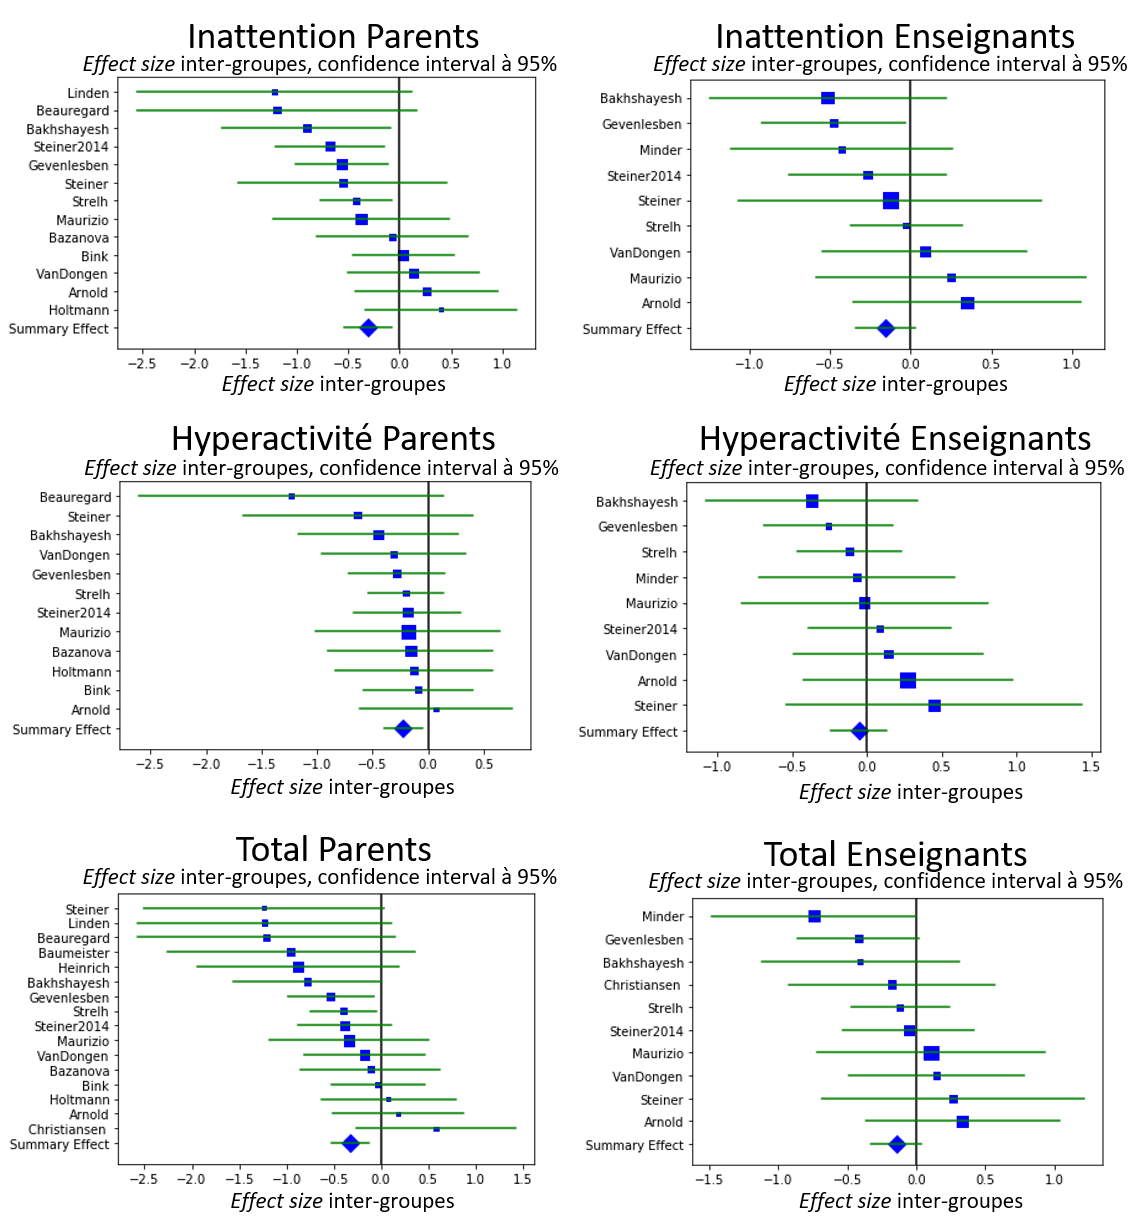
\includegraphics[width=1\linewidth]{figures/chapter-2/meta-analysis-forest-plots} 
  \caption[\textit{Forest plots} de la mise à jour de \citet{Cortese2016}.]{\textit{Forest plots} des \gls{es}-inter-groupes (les carrés bleus) avec 
	leur intervalle de confiance à 95\% (en vert) obtenus après la mise à jour de 
	\citet{Cortese2016}. Le losange bleu correspond à l'\gls{est}.
	Un \gls{es}-inter-groupes négatif est en faveur du \gls{nfb}.}
  \label{Figure:meta_analysis_forest_plots}
\end{figure}

Afin de détecter un biais de publication, une hétérogénéité parmi les études incluses ou la faible qualité méthodologique de certaines études, 
deux \textit{funnel plot} basés sur les \gls{es}-inter-groupes calculés sur les évaluations des symptômes totaux par les parents et les enseignants sont 
tracés à la Figure~\ref{Figure:meta_analysis_funnel_plots}. 

\begin{figure}[h!]
  \centering
	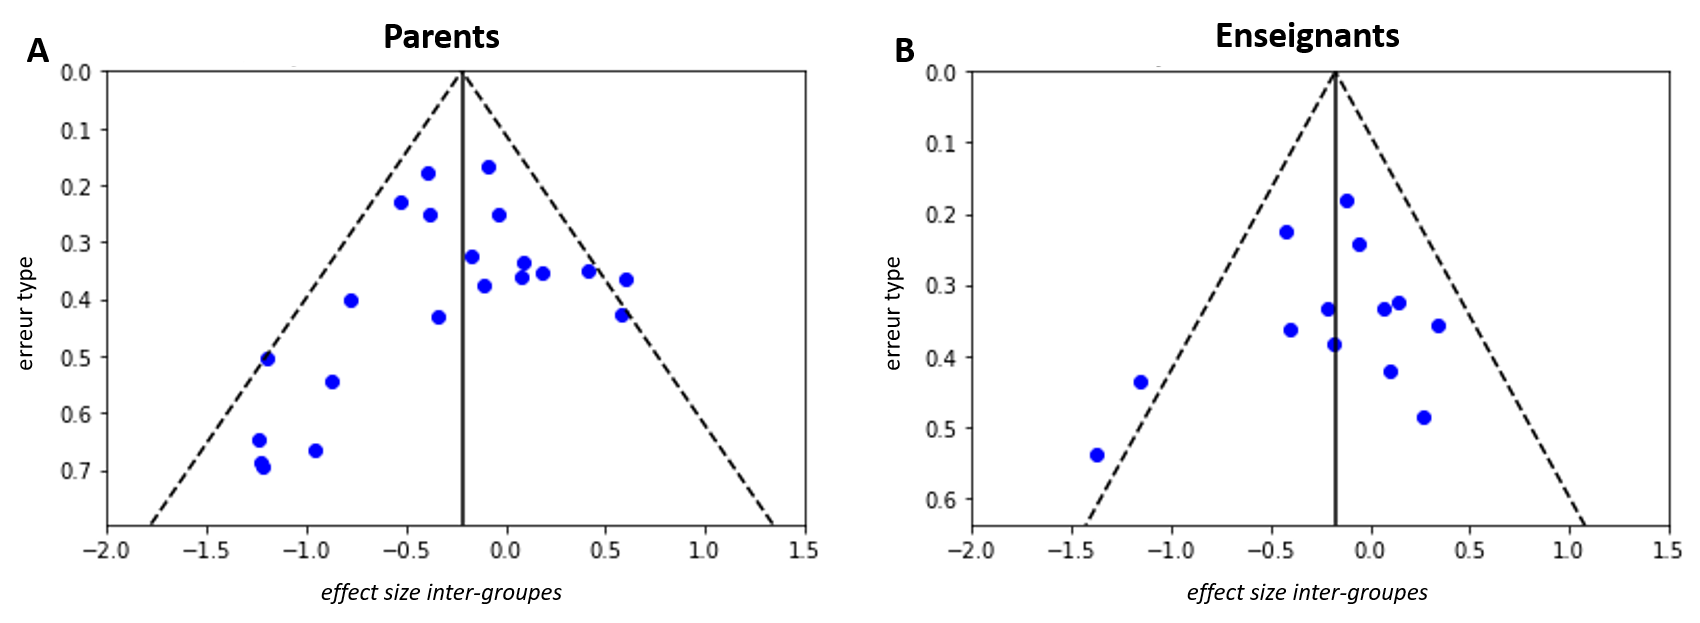
\includegraphics[width=1\linewidth]{figures/chapter-2/meta-analysis-funnel-plots} 
  \caption[\textit{Funnel plots} de la mise à jour de \citet{Cortese2016}.]{\textit{Funnel plots} obtenus pour les \gls{es}-inter-groupes calculés 
	sur les évaluations des symptômes totaux par les parents (en \textbf{A}) et 
	les enseignants (en \textbf{B}) avec un intervalle de confiance à 95\%.}
  \label{Figure:meta_analysis_funnel_plots}
\end{figure}

Visuellement, alors que le \textit{funnel plot} correspondant aux \gls{est} des enseignants semble plutôt symétrique, celui des parents parait asymétrique. 
Pour plus de précision, le test d'Egger a également été utilisé pour déterminer statistiquement si un biais s'est glissé dans l'analyse \citep{Egger1997} :
\begin{description}
\item[pour les parents :] contrairement à ce qui est observé, le \textit{funnel plot} n'est pas asymétrique, l'\textit{intercept} ne diffère pas 
significativement de 0 ($p$-value = 0.264),
\item[pour les enseignants :]  le \textit{funnel plot} n'est pas non plus asymétrique ($p$-value = 0.543).
\end{description}

Les études en dehors des pseudo limites de confiance à 95\% de l'\gls{est} sous le modèle à effet fixe sont : 
\begin{itemize}
\item pour les parents : \citet{Christiansen2014}, 
\item pour les enseignants : \citet{Moreno2019, Shereena2019}. 
\end{itemize}
 
\subsubsection{Résultats de la mise à jour sur les sous-groupes}
 
En ce qui concerne le sous-groupe \emph{protocole standard}, seul l'\gls{est} de la composante totale évaluée par les parents est significatif ($p$-value = 0.047). 
L'\gls{est} calculé pour la composante totale évaluée par les enseignants est limite significatif ($p$-value = 0.053).

Le sous-groupe \emph{pas de traitement médicamenteux en simultané} ne présente que l'\gls{est} de la composante inattention évaluée par les parents de 
significatif ($p$-value = 0.017).

\section{Discussion} 

Les méta-analyses doivent être menées rigoureusement, ainsi pour guider les auteurs des recommandations existent comme celles de PRISMA \citep{Moher2009}.
La réplication et la mise à jour présentées ici remplissent la majorité des points de cette \textit{checklist}, sauf notamment l'évaluation du risque de biais dans chaque étude.
Par ailleurs, elles ont été effectuées avec le package Python dont la fiabilité n'a été testée que sur une méta-analyse.
 
Le travail décrit précédemment a pour but d'explorer l'impact de certains choix de \citet{Cortese2016} qui ont été débattus dans la communauté scientifique 
\citep{Micoulaud2016}. Nous résumons ici la liste des changements, leur justification et leurs conséquences sur les résultats puis mettons en évidence 
les contributions de la mise à jour de la méta-analyse. 

\subsection{Discussion sur les résultats obtenus} \label{replication_and_update}

Les résultats obtenus suite à la réplication et à la mise à jour de \citet{Cortese2016} sont analysés et mis en perspective avec la littérature existante.

\subsubsection{Réplication}

Un des choix qui a été fait ici est d'utiliser la Conners-3 Teachers \citep{Conners2008} plutôt que la BOSS Classroom \citep{Shapiro2010} 
pour calculer les \gls{es}-inter-groupes obtenus par les évaluations des enseignants du fait de son utilisation plus commune \citep{Christiansen2014, Bluschke2016}.
Toutefois, l'utilisation de l'une ou l'autre de ces échelles ne change pas la significativité statistique des \gls{est} calculés pour les enseignants. 

La seconde différence entre \citep{Cortese2016} et la réplication effectuée ici est que le calcul des \gls{es}-inter-groupes de \citet{Arnold2014} se base 
sur les valeurs à post-test obtenues après 40 sessions de \gls{nfb} au lieu de valeurs temporaires obtenues après 12 sessions. Des études montrent
que le nombre de sessions est corrélé positivement avec les changements observés sur l'\gls{eeg} \citep{Vernon2004}, ainsi un faible nombre de sessions mènerait
à des \gls{es}-inter-groupes plus petits. Or, ici étonnament les \gls{es}-inter-groupes calculés après la réalisation de toutes les sessions sont plus faibles que ceux 
obtenus après 12 sessions, ce qui n'est pas favorable à l'efficacité du \gls{nfb}. Toutefois, ces différences ne changent pas la significativité statistique des \gls{est}. 

En conclusion, sur la base de cette étude de sensibilité, nous suggérons que les points de débat soulevés par \citet{Micoulaud2016} ne sont pas majeurs 
quant à l'analyse et l'interprétation des résultats obtenus.

\subsubsection{Mise à jour} \label{meta_analysis_update}

La méta-analyse de \citep{Cortese2016} a déjà fait l'objet d'une mise à jour présentée dans \citet{Bussalb2019clinical} qui a intégré les études de 
\citep{Bazanova2018, Baumeister2016} et \citet{Strehl2017}. Cette mise à jour confirmait les résultats de \citep{Cortese2016} : les \gls{est} calculés 
à partir des évaluations des parents sont en faveur de l'efficacité du \gls{nfb}, au contraire des évaluations des enseignants. 

Les résultats obtenus ici sont globalement les mêmes qu'après la mise à jour de \citet{Bussalb2019clinical} au niveau de la significativité statistique : la seule
différence importante est la perte de la significativité statistique de l'\gls{est} pour la composante hyperactivité évaluée par les parents ($p$-value = 0.069).
Les \gls{est} évalués par les enseignants sont, quant à eux, toujours non significatifs ($p$-value pour la composante totale =  0.09). 

Cette mise à jour conduit à des \gls{est} plus faibles en valeur absolue que ceux obtenus par \citet{Cortese2016} comme l'illustrent les \textit{forest plots} à 
la Figure~\ref{Figure:meta_analysis_forest_plots} : par exemple l'\gls{est} calculé pour la composante totale évaluée par les parents est de -0.23 alors
que la réplication de \citet{Cortese2016} résumée à la Table~\ref{Table:table_meta_review_comparison_replication_cortese} menait à un \gls{est} de -0.32.

La détection de biais dans cette mise à jour s'est déroulée en deux temps : une analyse visuelle des \textit{funnel plots} présentés à la Figure~\ref{Figure:meta_analysis_funnel_plots}
puis le test d'Egger. Aucun biais ne s'est immiscé dans les évaluations des enseignants ($p$-value du test d'Egger = 0.543) contrairement à ce qu'avaient trouvé \citet{Cortese2016} ($p$-value = 0.042). 
\citet{Cortese2016} avaient expliqué ce résultat non pas par la présence d'un biais de publication, mais par le fait que les plus petites études sont 
de moins bonne qualité et donc n'arrivent pas à montrer l'efficacité du \gls{nfb}. En effet, en cas de biais de publication, les résultats des petites
études auraient été en faveur du \gls{nfb}. 

En ce qui concerne les évaluations des parents, le \textit{funnel plot} parait asymétrique, or le test d'Egger contredit cette observation ($p$-value = 0.264). 
Cela pourrait s'expliquer par le faible poids associé aux études qui causent cette asymétrie visuelle. 

Enfin, l'ajout de ces sept nouvelles études donne plus de puissance statistique aux résultats, notamment pour l'analyse des sous-groupes menée par \citet{Cortese2016}.

En effet, pour la sous population suivant un protocole \gls{nfb} standard \citep{Arns2014}, \citet{Cortese2016} avaient noté que les \gls{pblind} observaient
une différence statistiquement significative entre le \gls{nfb} et les groupes contrôles en faveur du \gls{nfb}. Alors que cette tendance a été confirmée avec l'ajout 
de \citet{Baumeister2016} et \citet{Strehl2017} dans \citet{Bussalb2019clinical}, la mise à jour présentée ici rend presque tous les \gls{est} initialement significatifs 
non significatifs ; désormais seul l'\gls{est} de la composante totale évaluée par les parents l'est encore ($p$-value = 0.047). 
L'\gls{est} calculé pour la composante totale évaluée par les enseignants est limite significatif ($p$-value = 0.053). Ces résultats remettent en question l'efficacité
supérieure des protocoles standards.

En ce qui concerne le sous-groupe constitué d'études qui interdisent la prise de médicaments, la seule différence avec \citep{Cortese2016} est la perte de   
significativité statistique de l'\gls{est} de la composante hyperactivité évaluée par les parents ($p$-value = 0.062).

\subsection{Hétérogénéité des études} 

Même si les méta-analyses regroupent les études répondant toutes aux critères d'inclusion comme, par exemple, ceux énoncés à \ref{selection_studies}, 
elles diffèrent tout de même sur de nombreux points, comme le nombre de sessions et la durée du traitement, limitant la fiabilité de leurs résultats 
comme le soulignent \citet{Alkoby2017}. Afin de pallier 
cette hétérogénéité, l'analyse peut cibler une population plus précise, comme ce qui a été effectué lors de l'analyse
des sous populations. Cependant, ce genre de restriction souffre d'une puissance statistique plus faible et regroupe encore des études fortement hétérogènes.
En effet, même si seuls les protocoles \gls{scp}, \gls{tbr} et \gls{smr} sont utilisés, ils restent intrinsèquement différents et il est probable que leur
efficacité ne soit pas la même. 

Par ailleurs, le matériel d'acquisition utilisé, ainsi que le traitement du signal varient d'une étude à l'autre, or ces points sont sans doute centraux 
dans la performance du traitement. 

De plus, aucun consensus n'existe quant au nombre de sessions ou à la durée du traitement, ainsi ces choix sont très variables d'une étude à l'autre et peu
souvent questionnés, bien qu'ils soient centraux dans la théorie de l'apprentissage.

\section{Importance de la mise à jour des méta-analyses} \label{need_to_update_meta_analysis}

Afin d'éviter de tomber dans le \textit{p-hacking}, c'est à dire faire en sorte d'obtenir un résultat significatif, il est important de ne pas arrêter la collecte de données 
et donc de figer les résultats une fois que la $p$-value de l'\gls{est} passe sous le seuil de signicativité de 0.05 \citep{Head2015, Coffman2015}. En effet, l'arrêt prématuré des résultats peut
générer un biais : par exemple la $p$-value peut être significative à un instant $t$ avec un certain nombre de sujets inclus, puis perdre sa significativité statistique à
$t + 1$ et ne plus la retrouver. Ces deux configurations sont représentées avec des données factices à la Figure~\ref{Figure:meta-analysis-evolution-p-value-examples}.

\begin{figure}[h!]
  \centering
	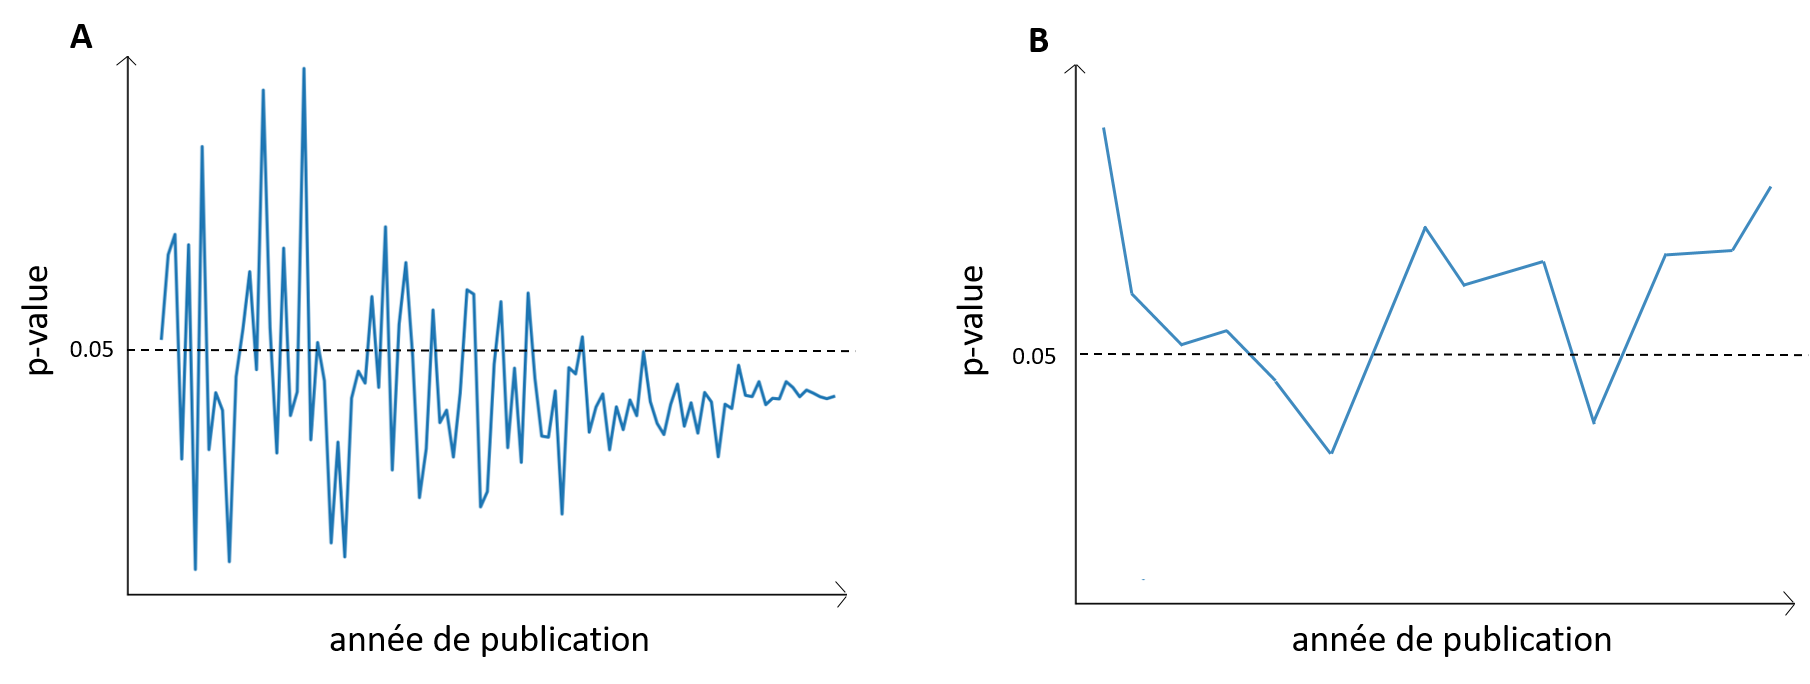
\includegraphics[width=1\linewidth]{figures/chapter-2/meta-analysis-evolution-p-value-examples} 
  \caption[Exemples d'évolution des $p$-value d'\gls{est} factices au fur et à mesure que la taille de l'échantillon augmente.]
	{Exemples d'évolution des $p$-value d'\gls{est} factices au fur et à mesure que la taille de l'échantillon augmente. 
	En \textbf{A}, la $p$-value se stabilise visuellement sous le seuil de significativité statistique suite à l'ajout de nouveaux sujets ; en \textbf{B}, la $p$-value 
	passe temprorairement sous le seuil de significativité puis s'en éloigne suite à l'ajout de nouveaux sujets. 
	Le seuil de significativité statistique à 5\% est représenté en pointillés noirs.}
  \label{Figure:meta-analysis-evolution-p-value-examples}
\end{figure}

Les conclusions d'une méta-analyse pourraient donc souffrir de l'arrêt prématuré des analyses lorsque la $p$-value de l'\gls{est} n'est pas stable. 
Ainsi, la méta-analyse de \citet{Cortese2016} a déjà fait l'objet de deux mises à jour, dont les différences vont être comparées par la suite : 
la première a été publiée en 2019 \citep{Bussalb2019clinical} et la deuxième est présentée en \ref{selection_studies}. 

\subsection{Mise en évidence de l'importance des mises à jour} \label{methods_importance_to_update_meta_analysis}

L'importance de mettre à jour les méta-analyses est étudiée en deux temps :
\begin{itemize}
\item par l'évolution de l'\gls{est} calculé sur la composante totale au fur et à mesure de l'inclusion des études selon leur année de publication ; l'intervalle de confiance à 95\% est 
aussi représenté,
\item par l'évolution de la $p$-value de ces \gls{est} ; l'intervalle de confiance à 95\% des $p$-values
est obtenu avec les $p$-values de chaque étude incluse. Une fois cet intervalle, noté CI, obtenu, ses bornes sont ajustées de façon à prendre en compte le fait 
que la $p$-value est une valeur bornée entre 0 et 1 \citep{Mandelkern2002} : 
\begin{equation}
\label{eq:metareview_confidence_interval_evolitio_p_value}
\text{CI} = \begin{cases}
           [max(0;\text{borne inférieure}) ; max(0;\text{borne supérieure})], \\
					 [min(1;\text{borne inférieure}) ; min(1;\text{borne supérieure})].
					  \end{cases}
\end{equation}
\end{itemize}

L'évolution des \gls{est} est considérée comme stable lorsque visuellement elle semble converger. Quant à l'évolution des $p$-values, elle est
estimée stable lorsque les bornes de son intervalle de confiance sont au-dessus (ou en-dessous) du seuil de significativité à 5\%.

Les courbes sont tracées pour les évaluations des parents (\gls{mprox}) et des enseignants (\gls{pblind}). Le nombre de sujets par étude (NS) et cumulatif (NSC) sont précisés sur les axes 
des abscisses en haut de chaque graphique. Les NSC sont obtenus de la façon suivante : $\text{NSC}(k) = \text{NSC}(k - 1) + \text{NS}(k)$, avec $k$ l'indice de l'étude incluse
allant de $1$ à $K$, avec $K$ le nombre total d'études incluses.
 
Par ailleurs, la réplication de la méta-analyse de \citet{Cortese2016} ainsi que ses mises
à jour sont symbolisées sur les tracés par une étoile si l'\gls{est} est statistiquement significatif ou par un carreau sinon : les symboles
rouges correspondent aux résultats de la réplication de \citet{Cortese2016} (cf. \ref{replication}), les verts à ceux de \citet{Bussalb2019clinical} et les violets à ceux de la mise à jour décrite en \ref{selection_studies}. Les méta-analyses
étant généralement publiées quelque temps après la fin de la sélection des études, leur année de publication est représentée grâce à un point de la même couleur que le carreau ou
l'étoile relié au résultat de la méta-analyse par une droite en pointillés. 

L'axe des ordonnées a été inversé de façon à ce que les points en hauteur correspondent aux méta-analyses les plus favorables au traitement.

Tous les \gls{est} obtenus ont été calculés à l'aide du package Python développé pour mener les analyses décrites dans ce chapitre
\citep{Bussalb2019clinical} et avec les choix qui ont été faits lors la réplication de la méta-analyse de \citet{Cortese2016} présentée en \ref{replication}.


\subsection{Analyse des courbes de l'évolution de la taille d'effet totale}

La Figure~\ref{Figure:meta_analysis_evolution_est_total} représente l'évolution de l'\gls{est} calculé grâce aux évaluations des parents (en \textbf{A}) et des 
enseignants (en \textbf{B}) sur la composante totale en fonction de l'année de publication des études satisfaisant le critère d'inclusion établi par \citep{Cortese2016} et énoncé en 
\ref{selection_studies}.

\begin{figure}[t]
  \centering
	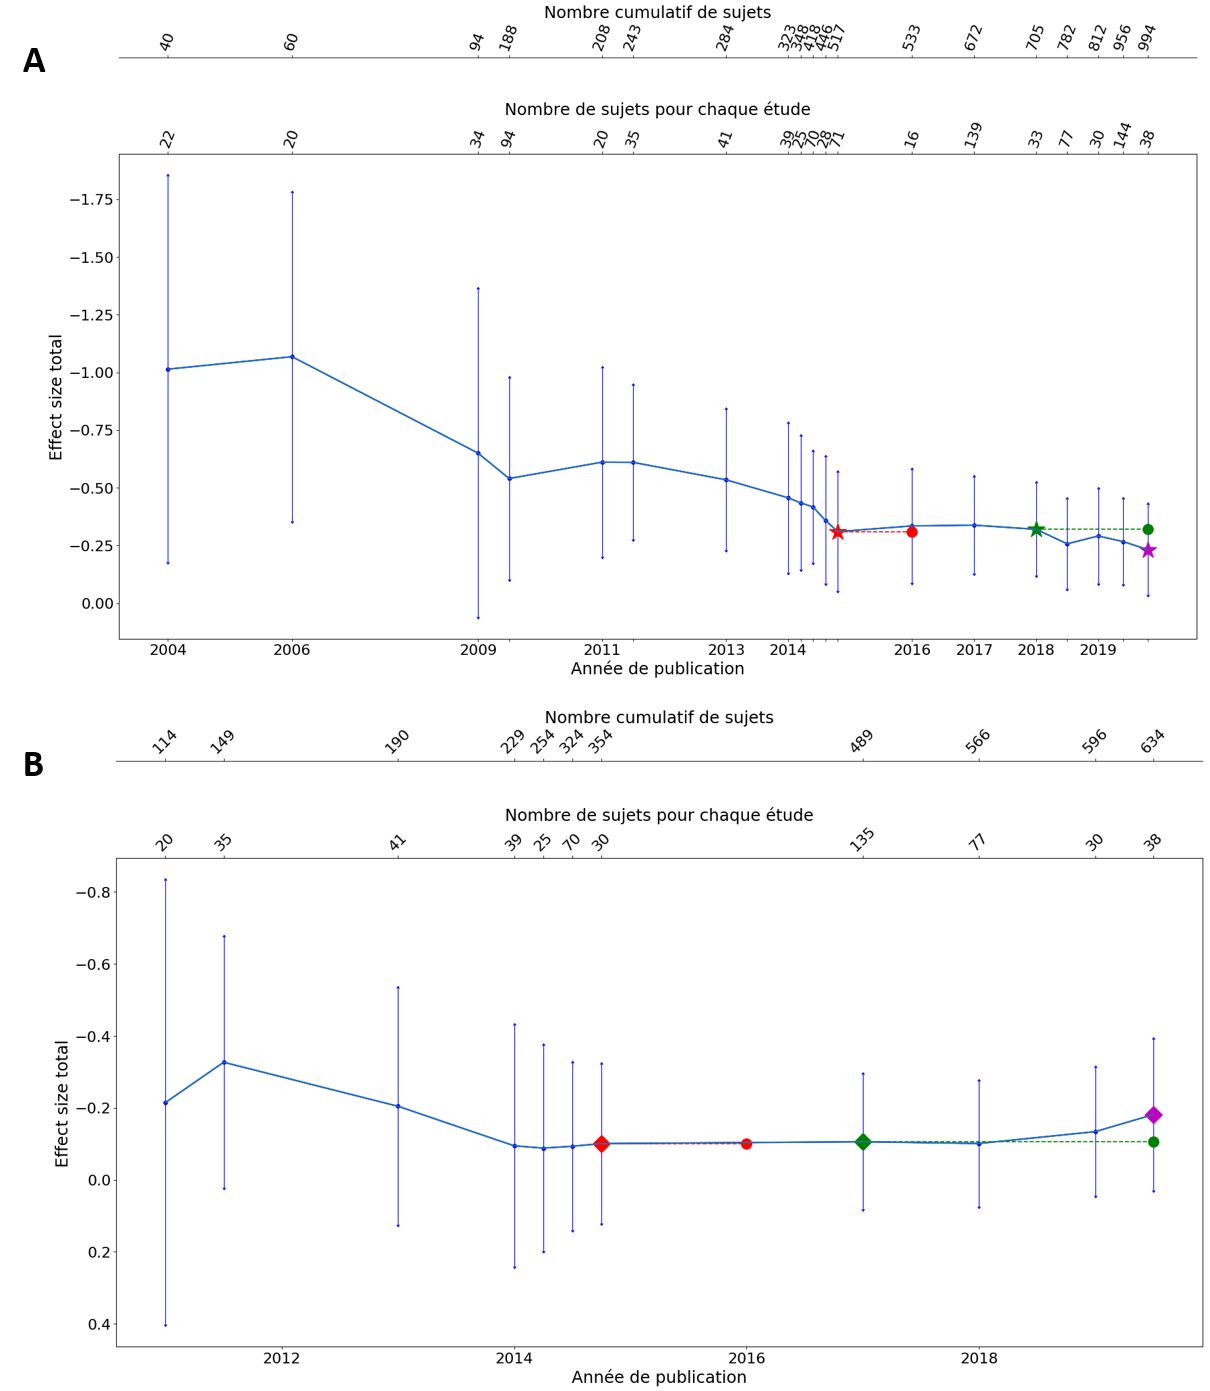
\includegraphics[width=1\linewidth]{figures/chapter-2/meta-analysis-evolution-summary-effect-total} 
  \caption[Evolution des \gls{est} au fur et à mesure de l'ajout de nouvelles études.]{Evolution des \gls{est} et de leur intervalle de confiance à 95\% au fur et à mesure de l'ajout des études satisfaisant le critère d'inclusion de \citet{Cortese2016} pour les évaluations des 
	parents en \textbf{A} et des enseignants en \textbf{B} sur la composante totale.
  Les résultats de la réplication de \citet{Cortese2016} sont représentés par des symboles rouges, ceux de \citet{Bussalb2019clinical} en vert et ceux présentés en \ref{selection_studies} en violet. Les étoiles 
	indiquent un \gls{est} statistiquement significatif, un losange un \gls{est} non statistiquement significatif. L'année de publication de ces méta-analyses est représentée grâce à un point de la couleur 
	d'intérêt relié au résultat de la méta-analyse par une droite en pointillés.
	Plus la valeur absolue de l'\gls{est} est élevée plus le traitement est efficace.
	Le nombre de sujets inclus par étude et cumulatif est indiqué sur les axes des abscissses supérieurs. La manière dont est calculé ce dernier est 
	décrite en \ref{methods_importance_to_update_meta_analysis}}
  \label{Figure:meta_analysis_evolution_est_total}
\end{figure}

Les \gls{est} obtenus grâce aux évaluations des parents (\textbf{A} de la Figure~\ref{Figure:meta_analysis_evolution_est_total}) varient de façon 
importante lorsque peu d'études sont incluses notamment entre 2006 et 2009, puis commencent à se stabiliser à 
partir de 2015, même si la valeur absolue des \gls{est} continue à diminuer. Les intervalles de confiance soulignent également cette stabilisation : ils diminuent 
avec l'augmentation du nombre d'études incluses. 

Cette tendance est également visible du côté des enseignants (\textbf{B} de la Figure~\ref{Figure:meta_analysis_evolution_est_total}). Toutefois, à partir 
de fin 2018 la valeur absolue des \gls{est} augmente.

Les mêmes graphiques sont tracés à la Figure~\ref{Figure:meta_analysis_evolution_est_std} mais cette fois en incluant seulement 
les études suivant un protocole standard \citep{Arns2014}.

\begin{figure}[t]
  \centering
	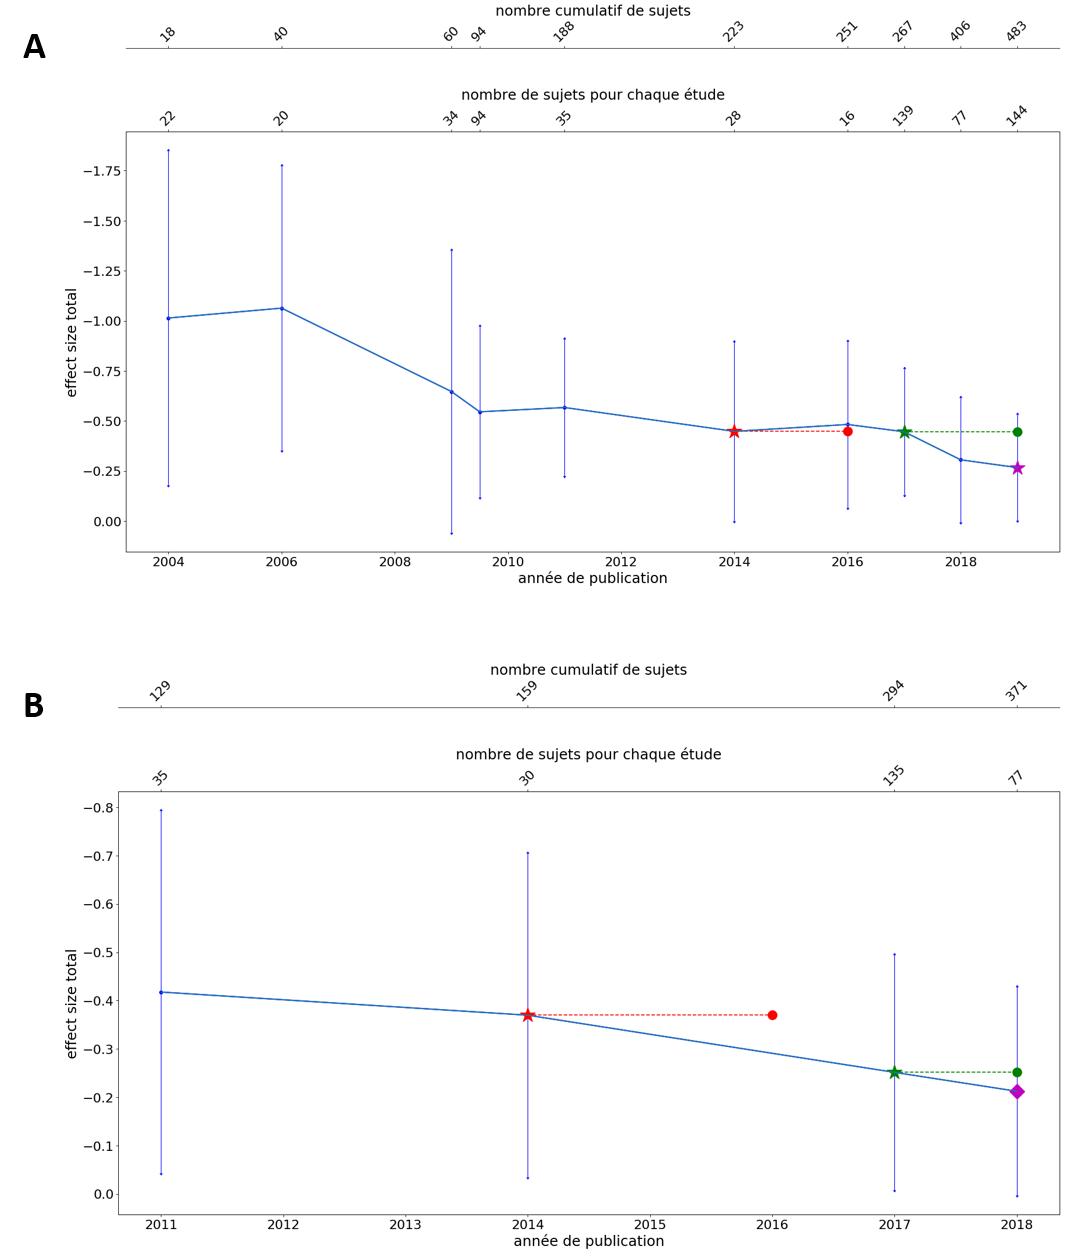
\includegraphics[width=1\linewidth]{figures/chapter-2/meta-analysis-evolution-summary-effect-std} 
  \caption[Evolution des \gls{est} au fur et à mesure de l'ajout de nouvelles études suivant un protocole standard.]{Evolution des \gls{est} et de leur 
	intervalle de confiance à 95\% au fur et à mesure de l'ajout des études suivant un protocole standard pour les évaluations des 
	parents en \textbf{A} et des enseignants en \textbf{B} sur la composante totale.
  Les résultats de la réplication de \citet{Cortese2016} sont représentés par des symboles rouges, ceux de \citet{Bussalb2019clinical} en vert et ceux présentés en \ref{selection_studies} en violet. Les étoiles 
	indiquent un \gls{est} statistiquement significatif, un losange un \gls{est} non statistiquement significatif. L'année de publication de ces méta-analyses est représentée grâce à un point de la couleur 
	d'intérêt relié au résultat de la méta-analyse par une droite en pointillés.
	Plus la valeur absolue de l'\gls{est} est élevée plus le traitement est efficace.
	Le nombre de sujets inclus par étude et cumulatif est indiqué sur les axes des abscissses supérieurs. La manière dont est calculé ce dernier est 
	décrite en \ref{methods_importance_to_update_meta_analysis}}
  \label{Figure:meta_analysis_evolution_est_std}
\end{figure}

\clearpage

Dans le cas des études satisfaisant la définition du protocole standard, les \gls{est} calculés à partir des évaluations des parents 
(\textbf{A} de la Figure~\ref{Figure:meta_analysis_evolution_est_std}) diminuent avec le temps, tout comme leur intervalle de confiance à 95\%. 
En ce qui concerne les \gls{est} obtenus grâce aux enseignants (\textbf{B} de la Figure~\ref{Figure:meta_analysis_evolution_est_std}), un faible nombre d'études 
est inclus et, alors que dans les cas précédents la diminution de l'\gls{est}ne menait pas à une perte de significativité statistique parmi les méta-analyses, 
ici la mise à jour de \citet{Cortese2016} présentée en \ref{selection_studies} conduit à un \gls{est} non significativement en faveur du \gls{nfb}. 

\subsection{Analyse des courbes de l'évolution de la $p$-value des tailles d'effet totales}

L'évolution des $p$-value de ces \gls{est} en fonction des études incluses est ensuite étudiée et présentée à la Figure~\ref{Figure:meta_analysis_evolution_pvalue_total} pour 
l'intégralité des études et à la Figure~\ref{Figure:meta_analysis_evolution_pvalue_std} pour les études suivant un protocole standard \citep{Arns2014}.

\begin{figure}[t]
  \centering
	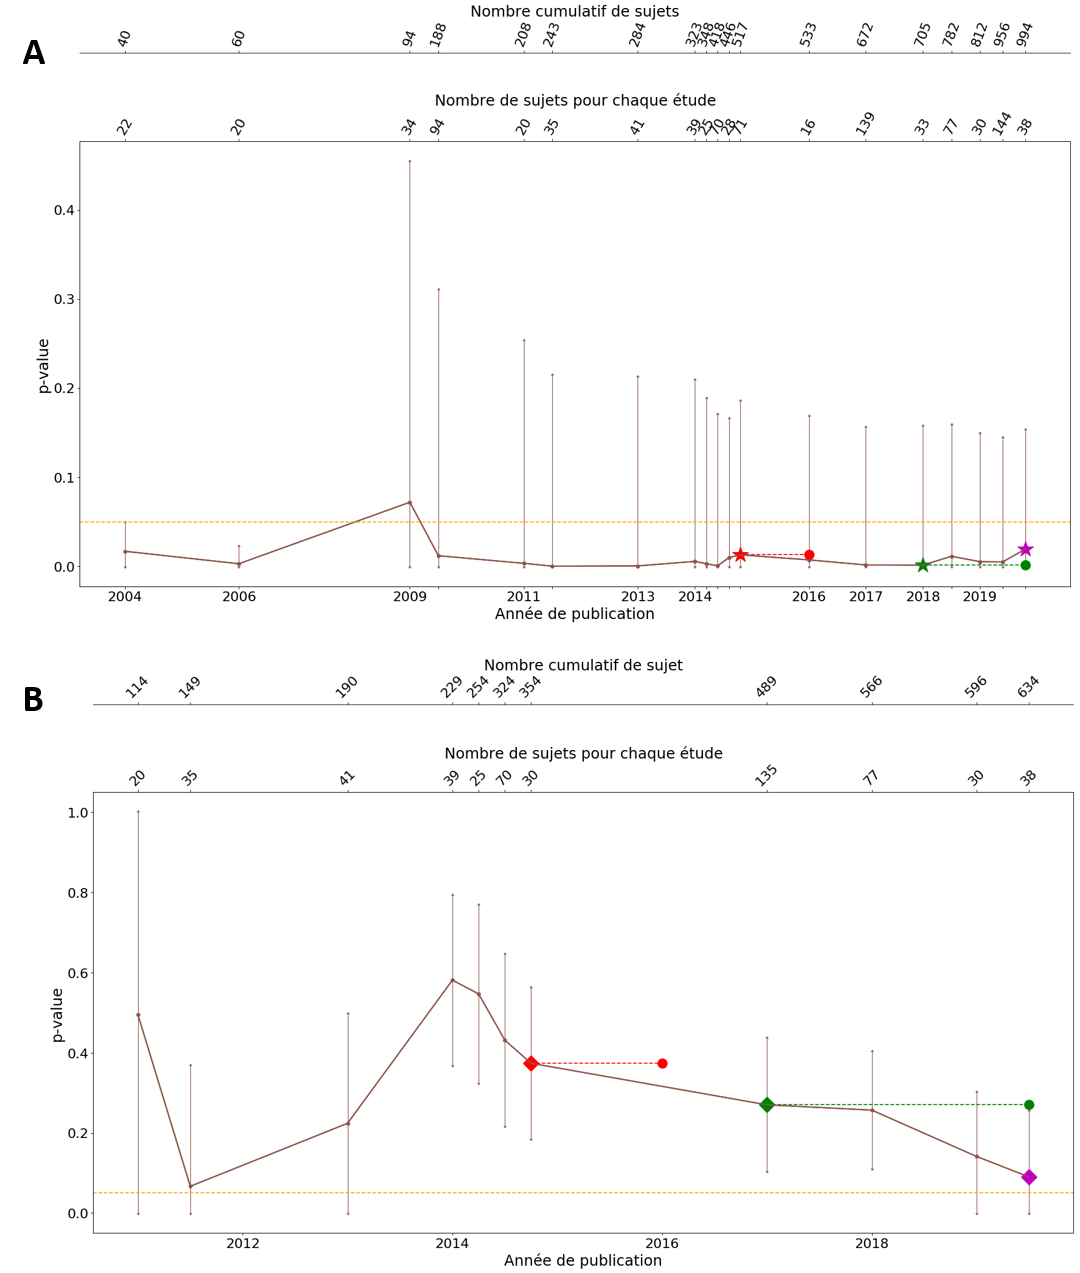
\includegraphics[width=1\linewidth]{figures/chapter-2/meta-analysis-evolution-pvalue-total} 
  \caption[Evolution de la $p$-value des \gls{est} au fur et à mesure de l'ajout de nouvelles études.]{Evolution de la $p$-value des \gls{est} et de leur intervalle de confiance à 95\% au fur et à mesure de l'ajout des études satisfaisant le critère d'inclusion de \citet{Cortese2016} pour les évaluations des 
	parents en \textbf{A} et des enseignants en \textbf{B} sur la composante totale.
  Les résultats de la réplication de \citet{Cortese2016} sont représentés par des symboles rouges, ceux de \citet{Bussalb2019clinical} en vert et ceux présentés en \ref{selection_studies} en violet. Les étoiles 
	indiquent un \gls{est} statistiquement significatif, un losange un \gls{est} non statistiquement significatif. L'année de publication de ces méta-analyses est représentée grâce à un point de la couleur 
	d'intérêt relié au résultat de la méta-analyse par une droite en pointillés.
	Le nombre de sujets inclus par étude et cumulatif est indiqué sur les axes des abscissses supérieurs. La manière dont est calculé ce dernier est 
	décrite en \ref{methods_importance_to_update_meta_analysis}
	Le seuil de significativité à 5\% est représenté par des pointillés orange.}
  \label{Figure:meta_analysis_evolution_pvalue_total}
\end{figure}

\begin{figure}[t]
  \centering
	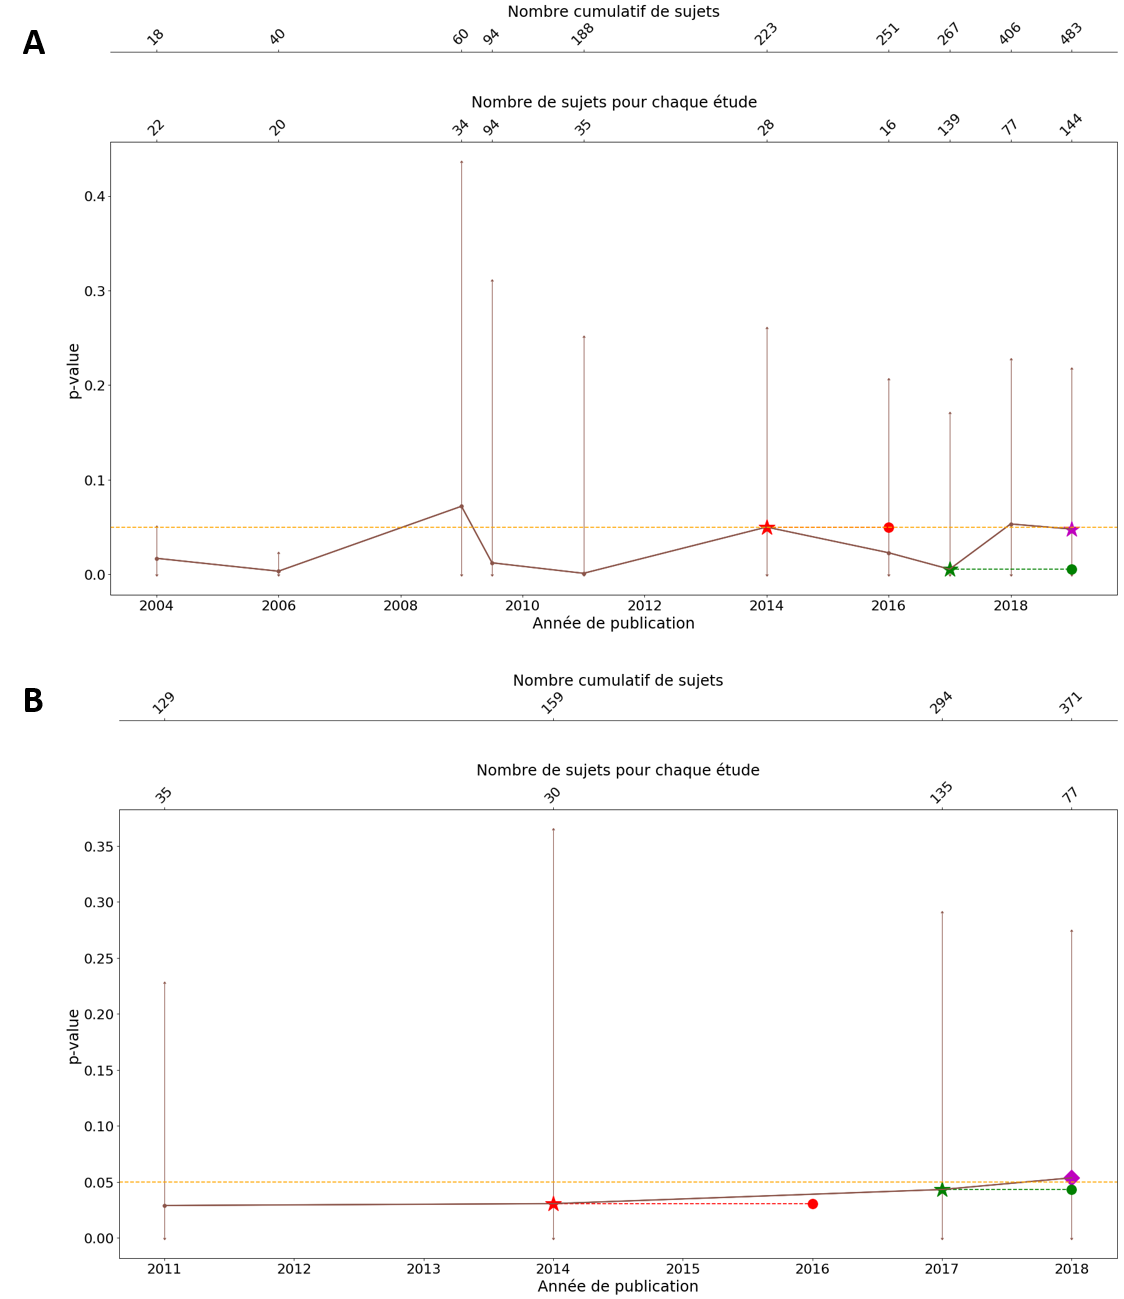
\includegraphics[width=1\linewidth]{figures/chapter-2/meta-analysis-evolution-pvalue-std} 
  \caption[Evolution de la $p$-value des \gls{est} au fur et à mesure de l'ajout de nouvelles études suivant un protocole standard.]{Evolution de la $p$-value 
	des \gls{est} et de leur intervalle de confiance à 95\% au fur et à mesure de l'ajout des études répondant à la définition du protocole standard pour les évaluations des 
	parents en \textbf{A} et des enseignants en \textbf{B} sur la composante totale.
  Les résultats de la réplication de \citet{Cortese2016} sont représentés par des symboles rouges, ceux de \citet{Bussalb2019clinical} en vert et ceux présentés en \ref{selection_studies} en violet. Les étoiles 
	indiquent un \gls{est} statistiquement significatif, un losange un \gls{est} non statistiquement significatif. L'année de publication de ces méta-analyses est représentée grâce à un point de la couleur 
	d'intérêt relié au résultat de la méta-analyse par une droite en pointillés.
	Le nombre de sujets inclus par étude et cumulatif est indiqué sur les axes des abscissses supérieurs. La manière dont est calculée ce dernier est 
	décrite en \ref{methods_importance_to_update_meta_analysis}.
	Le seuil de significativité à 5\% est représenté par des pointillés orange.}
  \label{Figure:meta_analysis_evolution_pvalue_std}
\end{figure}

\clearpage

Tout d'abord, en ce qui concerne l'évolution de la $p$-value en incluant l'intégralité des études pour les 
évaluations des parents (\textbf{A} de la Figure~\ref{Figure:meta_analysis_evolution_pvalue_total}), on remarque que les $p$-values sont toutes
en-dessous du seuil de significativité à 5\% sauf en 2009. Après 2009, les $p$-values varient moins et leur intervalle de confiance à 95\% diminue, 
ce qui laisse penser que nous sommes plutôt dans le cas \textbf{A} illustré à la Figure~\ref{Figure:meta-analysis-evolution-p-value-examples}. Toutefois,
la borne supérieure de l'intervalle de confiance n'est jamais en-dessous du seuil de significativité de 5\%.

Quant à l'évolution des $p$-values présentée en \textbf{B} de la Figure~\ref{Figure:meta_analysis_evolution_pvalue_total}, elle est
toujours non statistiquement significative, mais perd sa stabilité à partir de 2019.

Enfin, en ce qui concerne le groupe standard présenté à Figure~\ref{Figure:meta_analysis_evolution_pvalue_std}, les fluctuations des $p$-values 
sont moins importantes aussi bien pour les évaluations 
des parents (en \textbf{A}) que celles des enseignants (en \textbf{B}) mais restent instables. 
De plus, les $p$-values sont à la limite du seuil de significativité dans les deux cas lors de la dernière mise à jour.

\subsection{Discussion sur ces courbes}

Les courbes d'évolution des \gls{est} au fur et à mesure de l'inclusion de l'ensemble des études (Figure~\ref{Figure:meta_analysis_evolution_est_total}) 
illustrent le fait que l'\gls{est} 
devient visuellement de plus en plus stable avec le temps. Par ailleurs, la diminution des intervalles de confiance à 95\% montre que les résultats 
deviennent de plus en plus précis.

Les courbes correspondant à l'évolution de l'\gls{est} dans le sous-groupe des études suivant un protocole standard (Figure~\ref{Figure:meta_analysis_evolution_est_total}) 
fluctuent davantage du fait du nombre limité de sujets et d'études incluses.

Alors que les \gls{est} commencent dans l'ensemble à converger, leur $p$-value continue de fluctuer (Figure~\ref{Figure:meta_analysis_evolution_pvalue_total} et 
Figure~\ref{Figure:meta_analysis_evolution_pvalue_std}) même si sur la totalité des études elles s'accordent depuis 2011 sur la conclusion de \citet{Cortese2016} :
les évaluations des parents (\textbf{A} de la Figure~\ref{Figure:meta_analysis_evolution_pvalue_total}) sont significativement en faveur du \gls{nfb} 
au contraire des évaluations des enseignants (\textbf{B} de la Figure~\ref{Figure:meta_analysis_evolution_pvalue_total}). 
Toutefois, alors qu'elle était stable entre 2014 et 2018 pour les évaluations des enseignants, elle recommence à fluctuer à partir de 2019 : 
la $p$-value de la dernière mise à jour de \citet{Cortese2016} tend vers la significativité statistique, il serait donc intéressant 
de continuer à mettre à jour ce travail pour déterminer si cette $p$-value devient significative et le reste.

Dans le cas de l'évolution des $p$-values dans le sous-groupe des études suivant un protocole standard (Figure~\ref{Figure:meta_analysis_evolution_pvalue_std}), 
la dernière mise à jour 
de \citet{Cortese2016} conduit à des résultats limite significatifs pour les évaluations des parents (\textbf{A}) et à une perte de significativité statistique pour celles des 
enseignants (\textbf{B}), remettant en question les conclusions de \citet{Cortese2016} et \citet{Bussalb2019clinical} quant à l'efficacité des protocoles standards.
 
La $p$-value est très largement utilisée en méta-analyse, mais est également de plus en plus contestée du fait qu'elle soit trop souvent mal interprétée 
\citep{Halsey2019}. 
En effet, la $p$-value mesure le degré de compatibilité entre les données et l'hypothèse nulle, et non la probabilité que l'hypothèse nulle soit vraie

Ainsi, les chercheurs se tournent de plus en plus vers les statistiques bayésiennes, avec des outils comme le rapport de vraisemblance 
(\textit{likelihood ratio} en anglais) \citep{Dormuth2016}, ou le facteur de Bayes \citep{Morey2016, Rouder2011}. L'évolution de ces 
valeurs avec l'inclusion de nouvelles études serait intéressante à étudier. 

Pour conclure, la mise à jour des méta-analyses peut avoir une incidence sur la significativité statistique de la $p$-value, notamment dans le cas où peu d'études et donc de sujets
sont inclus. Continuer à inclure de nouvelles études permet d'augmenter la puissance statistque des calculs : en particulier les études les plus récentes sur l'efficacité du \gls{nfb}
appliqué aux enfants \gls{tdah} comportent de plus en plus de sujets.

Enfin, étant donné l'essor de l'utilisation du \gls{nfb} appliqué aux enfants \gls{tdah}, au moment de la publication d'une méta-analyse de nouvelles études satisfaisant ses critères d'inclusion
sont déjà disponibles comme illustré aux figures~\ref{Figure:meta_analysis_evolution_est_total} et ~\ref{Figure:meta_analysis_evolution_est_std}. Ainsi, à peine publiés, les résultats de la 
méta-analyse sont déjà obsolètes, ce qui appelle à leur mise à jour. 

Cette approche qui consiste à affiner les résultats à l'aide de nouvelles observations est l'une des bases de l'inférence bayésienne.

\section{Conclusion}

Cette partie s'est concentrée sur un outil couramment utilisé pour évaluer l'efficacité du \gls{nfb} : la méta-analyse. Ce travail a été l'occasion de mettre au point un package 
\textit{open-source} pour effectuer une méta-analyse en toute transparence et aider à la réplication ou à la mise à jour de ses résultats.

Ce package a justement été utilisé pour répliquer la méta-analyse de \citet{Cortese2016} dont certains points ont été discutés par la communauté scientifique. 
Il se trouve que les choix effectués par \citet{Cortese2016} s'avèrent anodins mais illustrent la complexité de l'émergence de la preuve
clinique.

Cette réplication a également mis en évidence l'importance de la disponibilité des données cliniques afin d'effectuer des calculs précis et de conclure de façon
plus fiable quant à l'efficacité d'un traitement. 

Il est important de noter qu'une méta-analyse ne rend compte de l'efficacité d'un traitement qu'à un moment donné : étant donné le nombre important d'études évaluant l'efficacité du \gls{nfb} 
pour les enfants souffrant du \gls{tdah}, mettre à jour les méta-analyses est nécessaire, c'est pourquoi un tel travail a été entrepris ici. Par ailleurs, l'analyse de l'évolution de l'\gls{est} et des $p$-values 
associées en fonction de l'ajout des études montrent que ces métriques tendent à se stabiliser depuis quelques années mais ne convergent pas encore, appelant à de nouvelles mises à jour.  

Les résultats des méta-analyses donnent une idée de l'efficacité du traitement étudié, même s'il faut garder à l'esprit que les études incluses
diffèrent sur différents points, ce qui est notamment vrai pour le \gls{nfb}. Afin de pallier cette faiblesse, des sous-groupes peuvent être étudiés comme ici avec le groupe d'études
suivant un protocole standard et celui d'études où les enfants ne prennent pas de médicaments.

Cependant cette approche ne gomme pas toutes les différences entre les études. Or, ces différences ont sans doute une influence sur l'efficacité du \gls{nfb}, ainsi nous proposons dans le chapitre 
suivant de tirer avantage de cette hétérogénéité entre les études pour tenter de mettre en évidence les facteurs 
techniques et/ou cliniques qui pourraient avoir une influence sur la performance du \gls{nfb}.

  
 
\newpage
\chapter{Identification des facteurs influençant l'efficacité du Neurofeedback} \label{ch-saob}

\section*{Introduction}

La réplication et la mise à jour de la méta-analyse de \citet{Cortese2016} décrite dans le chapitre précédent a permis de mettre en évidence la forte 
hétérogénéité des études incluses dans ce type d'analyse. En effet, même si ces études satisfont toutes des critères définis par les auteurs pour pouvoir
les inclure dans leur analyse, elles diffèrent d'un point de vue technique et méthodologique : elles ont été rassemblées sans tenir compte, par exemple, 
de la qualité de l'acquisition de l'\gls{eeg}, du neuromarqueur entrainé lors du \gls{nfb} et du design de l'étude clinique (notamment le nombre de sessions 
et la durée du traitement). 

Afin de mieux identifier l'importance de ces facteurs sur l'efficacité du \gls{nfb}, une nouvelle approche a été implémentée : l'analyse systématique des biais 
(\gls{saob} en anglais). Dans cette analyse, l'efficacité du traitement est considérée comme la variable dépendante expliquée par des variables indépendantes 
qui sont ici les facteurs méthodologiques et techniques. Le but de cette analyse est donc de déterminer les paramètres qui ont une influence sur la performance du 
\gls{nfb} afin de mieux les prendre en compte dans l'implémentation d'études cliniques évaluant l'efficacité. 
\clearpage

\section{Extraction et pré-traitement des facteurs}

La première étape de la \gls{saob} est d'obtenir les facteurs des études sélectionnées. Une liste de facteurs ayant potentiellement une influence sur 
l'efficacité du \gls{nfb} a été établie en \ref{choix_des_facteurs}. Ces facteurs ont ensuite été extraits de chaque étude. Avant de débuter l'analyse, ils ont été pré-traités en 
suivant les étapes décrites en \ref{preprocessing}. 

\subsection{Choix des facteurs} \label{choix_des_facteurs}

Tout d'abord, une revue de littérature et des discussions avec des experts du \gls{nfb} appliqué aux enfants \gls{tdah}, en particulier le Dr. Jean-Arthur Micoulaud Franchi
et le Dr. Louis Mayaud, ont permis de déterminer les facteurs dont il serait intéressant d'étudier l'influence \citep{Vernon2004, Arns2009, Arns2014, Cortese2016, Enriquez2017}. Ces facteurs sont, pour
la plupart, spécifiques à l'entrainement par \gls{nfb} et sont définis avec plus de précision en \ref{principe_nfb}.

Les paramètres ayant une possible influence sur l'efficacité perçue du \gls{nfb} ont été répartis en cinq catégories :
\renewcommand{\labelitemi}{$\bullet$}
\begin{itemize}
\item \emph{les biais méthodologiques :} 
    \begin{itemize} 
		\item la présence d'un groupe contrôle, 
		\item l'aveugle des évaluateurs (\gls{pblind}), 
		\item la randomisation des sujets dans les essais contrôlés,
		\item l'autorisation de conduire l'étude par un \gls{cpp} (\gls{irb} en anglais).
    \end{itemize}
Ces paramètres ne sont pas spécifiques de l'entrainenement par \gls{nfb} mais pourraient avoir une influence sur les résultats.
En effet, \citet{Ros2019} appellent notamment à employer un groupe contrôle et à avoir recours à des évaluateurs aveugles afin d'améliorer la qualité des études.
\item \emph{la population :} 
    \begin{itemize}
    \item la prise de psychostimulants durant le traitement par \gls{nfb}, 
		\item la tranche d'âge des enfants inclus, 
		\item la sévérité des symptômes du TDAH à pré-test (score clinique à pré-test divisé par le score maximal à atteindre sur l'échelle clinique), 
		\item le degré d'engagement dans l'entrainement par \gls{nfb} (observance thérapeutique et ressenti vis à vis du traitement).
    \end{itemize}
Certaines de ses caractéristiques ont déjà été étudiées, en particulier l'impact de la prise de psychostimulants durant l'entrainement par \gls{nfb} dans
\citet{Cortese2016} et ses mises à jour (\citep{Bussalb2019clinical} et celle en \ref{selection_studies}) et également discuté par \citet{VanDoren2017}.
\item \emph{l'implémentation du \gls{nfb} :} 
    \begin{itemize}
    \item le protocole utilisé (\gls{scp}, \gls{smr}, l'augmentation du rythme theta, l'augmentation du rythme beta dans les aires centrale ou frontale 
    et la diminution du rythme theta), 
		\item la présence d'une phase de transfert lors de l'entrainement par \gls{nfb} (bloc durant lequel aucun \textit{feedback} n'est délivré), 
		\item l'utilisation d'une méthodologie de transfert d'apprentissage (pour s'entrainer à la maison ou à l'école), 
    \item le type de seuillage pour les récompenses discrètes (le seuil qui permet l'attribution des récompenses peut avoir une valeur fixe tout au long du traitement ou bien variable
		selon les performances de l'enfant), 
		\item le nombre de sessions de \gls{nfb}, 
		\item la durée et la fréquence des sessions, 
		\item la durée du traitement, 
		\item l'individualisation des bandes de fréquence basée sur l'\gls{iapf} (l'\gls{iapf} est la valeur du pic dans la bande alpha qui diffère selon les individus), 
		\item le couplage du \gls{nfb} avec l'\gls{emg}-Biofeedback (un retour est donné sur l'activité électrique du cerveau, mais aussi sur l'activité musculaire qui est 
		également enregistrée : l'enfant doit
		contrôler les deux simultanément).
		\end{itemize}
Il existe différents types de protocoles dont l'efficacité clinique a déjà été comparée précisément
\citep{Leins2007}. Les paramètres concernant l'aide au tranfert d'apprentissage semblent jouer un rôle important comme le soulignent \citet{Arns2014, Gani2008, Strehl2006}.
Par ailleurs, l'influence de ces facteurs sur le \gls{nfb} est étudiée à travers la méta-analyse de \citet{Cortese2016} et ses mises à jour en regroupant les études suivant un protocole standard
\citep{Arns2014}.

La question du seuil est également déterminante comme soulignée par \citet{Arns2014}. En ce qui concerne le nombre de sessions, ce paramètre a fait l'objet de plusieurs analyses \citep{Cortese2016, Arns2009,
Arns2014, Enriquez2017} afin de déterminer sa valeur optimale. La durée du traitement et des sessions ainsi que leur fréquence étant variables d'une étude à l'autre, il parait important
de les étudier. 

Enfin l'individualisation des bandes de fréquences et le couplage entre le \gls{nfb} et l'\gls{emg}-Biofeedback font l'objet de plus en plus d'études \citep{Bioulac2019, Bazanova2018, Bink2014,
Duric2012}, ainsi leur influence serait intéressante à explorer.
\item \emph{la qualité de l'acquisition :} 
    \begin{itemize}
    \item la présence de plus d'une électrode active (c'est à dire d'où est enregistré le signal duquel est extrait le neuromarqueur qui mènera au \textit{feedback}) et la qualité de 
		l'\gls{eeg}. Cette dernière est représentée par un indicateur allant de 1 à 3, calculé sur les critères suivants : 
        \begin{description} 
        \item[le type d'électrode utilisée :] les électrodes à gel,
        \item[le contrôle de l'impédance :] la vérification du bon contact entre la peau et les électrodes en gardant l'impédance inférieure à $40$k$\Omega$,
        \item[la certification du matériel hardware utilisé :] le matériel doit être conforme à la norme ISO-60601-2-26 \citep{ISO}.
        \end{description}
    Un score de qualité de 3 est donné si tous les critères ci-dessus sont remplis. Si au moins l'un d'eux est satisfait, le score est de 2, sinon il est mis à 1.
		\end{itemize}
Le matériel utilisé semble intuitivement être central quant à l'efficacité du \gls{nfb} d'où notre idée d'étudier son impact de plus près.
\item \emph{la qualité du signal} : 
    \begin{itemize}
    \item le rejet en temps réel (l'époque est exclue, pas de retour ou \emph{feedback} calculé) ou la correction (retour calculé sur l'époque débruitée) des 
artefacts oculaires (\gls{eog}),
    \item le rejet en temps réel d'artefacts génériques détectés grâce à leur large amplitude. 
    \end{itemize}
Le signal \gls{eeg} est l'élement central du \gls{nfb} et peut être très facilement contaminé par des artefacts \citep{Chavez2018}, ainsi l'effet de la correction ou du rejet 
d'atefacts est à étudier. 
\end{itemize}

Afin d'éviter tout biais d'analyse, le nom des facteurs a été caché durant toute l'analyse : il n'a été révélé qu'à la phase d'interprétation du modèle, lorsque ce dernier a été considéré 
comme valide notamment au niveau de la normalisation des variables et de la validation des hypothèses du modèle.  

\subsection{Pré-traitement des facteurs} \label{preprocessing}

Les auteurs des études incluses dans la \gls{saob} ne précisent pas systématiquement toutes les valeurs des facteurs, ce qui conduit à des observations manquantes. 
Afin que les paramètres pour lesquels peu d'observations sont disponibles ne faussent l'analyse, il est apparu raisonnable de considérer qu'au-delà de 20\%
d'observations manquantes ce paramètre est exclu. Les observations manquantes dans les facteurs comportant des valeurs numériques sont 
imputées et remplacées par -1.

Par ailleurs, comme cette analyse tire avantage de l'hétérogénéité des études, si un facteur a plus de 80\% d'observations identiques, 
celui-ci est également rejeté. 

Ces valeurs de seuil de 20\% et de 80\% ont été choisies arbitrairement.

Il est important de noter qu'une étude ne correspond pas nécessairement à une observation : lorsque plusieurs échelles cliniques et/ou évaluateurs sont disponibles dans une étude,
chaque couple échelle clinique-évaluateur est considéré comme une observation.

Ensuite, les facteurs qui sont des variables catégorielles (le protocole utilisé par exemple) sont codés en \textit{dummies} : la présence du facteur est représentée par un 1 et son absence par 0. 

Enfin, les variables sont standardisées : à chaque observation est soustraite la moyenne de l'ensemble des observations, le tout divisé par l'écart-type de la moyenne de 
l'ensemble des observations. La standardisation a été choisie plutôt que la normalisation afin de garder les valeurs extrêmes dans la \gls{saob} qui auraient été mises à 0 ou 1 avec 
la normalisation. 

Les facteurs sélectionnés et prétraités sont les variables indépendantes de l'analyse.

\section{Explication de l'efficacité du Neurofeedback par des méthodes multivariées}

Afin de déterminer quels facteurs parmi ceux sélectionnés précédemment ont une influence sur l'efficacité du \gls{nfb}, trois méthodes multivariées sont
utilisées : la \gls{wls}, le \gls{lasso} et le \gls{dt}. Ces méthodes ont pour but d'expliquer l'efficacité du \gls{nfb}, quantifiée par un \gls{es}
défini par la suite, à l'aide des facteurs. Les résultats de chaque méthode vont être combinés pour identifier quels paramètres sont susceptibles 
d'avoir un impact sur l'efficacité du \gls{nfb} appliqué aux enfants \gls{tdah}. 

\subsection{Calcul de la taille d'effet intra-groupe} \label{es_within}

L'efficacité du traitement est quantifiée par l'\gls{es}-intra-groupe. Celui-ci est calculé à partir des moyennes et écart-types des scores 
cliniques totaux donnés par les parents et les enseignants (considérés comme \gls{pblind} \citep{Sonuga-Barke2013, Micoulaud2014, Cortese2016}). De plus, 
lorsqu'une étude fournit des résultats pour plus d'une échelle clinique, l'\gls{es}-intra-groupe est calculé pour chaque échelle :
\begin{equation}
\label{eq:factors_effect_size_within_subject}
\text{ES-intra-groupe} = \frac{M_{\text{post},T} - M_{\text{pré},T}}{\sqrt{\frac{\sigma_{\text{pré},T}^2 + \sigma_{\text{post},T}^2}{2}}},
\end{equation} 
\noindent où $M_{\text{t},T}$ est la moyenne sur l'échelle clinique, pour le traitement $T$, au moment t (pré-test ou post-test) et $\sigma_{\text{t},T}$ représente
son écart-type. Au contraire de l'\gls{es}-inter-groupes défini à l'équation Eq.~(\ref{eq:metareview_effect_size_between}), cet \gls{es} permet de se concentrer sur l'effet du 
traitement au sein du groupe \citep{Cohen1988}. Cette définition de l'\gls{es} a déjà été précédemment utilisée dans la littérature sur le \gls{nfb} 
appliquée aux enfants \gls{tdah} \citep{Arns2009, Maurizio2014, Strehl2017}. Plus la valeur absolue de \gls{es}-intra-groupe est élevée, plus
le traitement étudié est efficace. 

Afin de limiter l'influence d'observations extrêmes parmi les valeurs des \gls{es}-intra-groupe, celles se trouvant à plus de 3 écart-types de la moyenne
de tous les \gls{es}-intra-groupe calculés ont été retirées de l'analyse \citep{Shewhart1931}.

Par la suite, l'ensemble des \gls{es}-intra-groupe est considéré comme la variable dépendante que les variables indépendantes (les facteurs) vont expliquer. 

\subsection{L'analyse systématique des biais}

La \gls{saob} comporte trois méthodes qui ont été implémentées à l'aide des bibliothèques Python Scikit-Learn \citep[version 0.18.1]{Pedregosa2011} et Statsmodels \citep[version 0.8.0]{Seabold2010} : 
\begin{itemize}
  \item une régression linéaire multiple et pondérée (\gls{wls} en anglais) \citep{Montgomery2012},
	\item une régression linéaire régularisée (\gls{lasso} en anglais) \citep{Tibshirani1996},
	\item un arbre de décision de régression (\gls{dt} en anglais) \citep{Quinlan1986}.
\end{itemize}

Les résultats de ces trois méthodes intrinsèquement différentes vont être combinés : si un facteur est identifié par les trois méthodes, alors son influence sur l'efficacité du 
\gls{nfb} est plus probable que si une seule méthode l'identifie. 

\subsubsection{La régression linéaire multiple et pondérée}
La régression linéaire a pour but d'estimer les coefficients de régression qui lient les facteurs aux \gls{es}-intra-groupe. Ici, la régression est pondérée pour, d'une part, 
prendre en compte le fait que, pour certaines études, plusieurs échelles cliniques sont disponibles, et d'autre part pour capturer les différentes tailles d'échantillon parmi les études.
Le poids $w_{i}$ associé à chaque observation $i$ est défini comme suit : 
\begin{equation}
\label{eq:weight_WLS}
w_{i} = \frac{\text{N}_{k}}{\text{NS}_{k}},
\end{equation} 
avec $\text{N}_{k}$  le nombre de sujets dans l'étude $k$ dans le groupe suivant le traitement et $\text{NS}_{k}$  le nombre 
d'échelles cliniques disponibles dans l'étude $k$ évaluant l'efficacité du traitement.

Mathématiquement, la \gls{wls} se traduit ainsi : 
\begin{equation}
\label{eq:factors_model_WLS}
\textbf{W}y = \textbf{WX}\beta + \epsilon.
\end{equation}
$\textbf{X}$ est une matrice inversible $(n \times p)$ et représente $n$ observations sur chaque $p-1$ variable indépendante et l'intercept, 
$\beta$ est un vecteur $(p \times 1)$ des coefficients de régression associés, $\textbf{W}$ est une matrice diagonale $(n \times n)$  
des poids $w_{i}$, $y$ est un vecteur $(n \times 1)$ des variables dépendantes et $\epsilon$ est un vecteur $(n \times 1)$ d'erreurs.

Le but de la \gls{wls} est d'estimer le vecteur de coefficients $\beta$ en minimisant la somme pondérée des carrés des résidus (\gls{wrss} en anglais) :
\begin{equation}
\label{eq:factors_WRSS}
\text{WRSS} = \sum_{i=1}^{n} w_i \Big(y_i - \beta_{0} - \sum_{j=1}^{p}\beta_{j}x_{ij}\Big)^2.
\end{equation}

Une fois le vecteur $\beta$ estimé, on cherche à savoir si les hypothèses du modèle sont vérifiées : 
\begin{itemize}
	\item la matrice ${\textbf{X}}^{T}\textbf{W}^{T}\textbf{WX}$ est régulière,
  \item aucune corrélation apparente n'est trouvée entre les variables indépendantes non catégorielles, 
  \item la tendance linéaire estimée est trouvée significative en se basant sur la statistique F,
  \item les résidus sont distribués normalement en se basant sur le kurtosis et le test Omnibus.
\end{itemize} 

Si toutes ces hypothèses sont satisfaites, alors les résultats de la \gls{wls} peuvent être interprétés. A l'aide d'un t-test, on détermine  
parmi les coefficients $\beta_{j}$ où $1<j<p$, ceux qui sont significativement différent de 0 (avec un seuil de significativité égal à 0.05) : 
pour ces coefficients, le facteur qui leur est associé est supposé avoir une influence sur l'efficacité du \gls{nfb}. Par ailleurs, 
le signe du coefficient indique si cette influence est positive ou négative. 

Etant donné le nombre important de variables indépendantes, le pourcentage de variance estimée par la \gls{wls} est quantifié par le coefficient de 
détermination ajusté (\textit{adjusted R-Squared} en anglais) plutôt que par le coefficient de détermination simple (\textit{R-Squared} en anglais).

Une régression linéaire ordinaire (\gls{ols} en anglais) est aussi mise en place pour observer l'impact des poids sur les résultats. 

\subsubsection{La régression linéaire régularisée}

La deuxième méthode appliquée lors de la \gls{saob} est le \gls{lasso} qui intègre la sélection de variables dans le modèle linéaire grâce à la norme $\ell_1$ appliquée aux coefficients.
Les coefficients $\hat{\beta}_{j}$ ($1<j<p$) sont obtenus en minimisant le coût :
\begin{equation}
\label{eq:factors_lasso-minimization}
\hat{\beta} = \argmin_\beta \sum_{i=1}^{n} \Big(y_i - \beta_{0} - \sum_{j=1}^{p}\beta_{j}x_{ij}\Big)^2 + \lambda \sum_{j=1}^{p}\abs{\beta_{j}},
\end{equation} 
où $\lambda$ est le paramètre de régularisation qui, en augmentant, met de plus en plus de coefficients à 0. 

Le paramètre de régularisation optimal est déterminé par une validation croisée \textit{leave-one-out}. Cette méthode prend une seule observation 
comme donnée de test pour la validation, laissant $n-1$ observations pour les données d'entraînement. Le processus de la validation croisée est ensuite répété $n$ fois pour que chaque observation 
soit utilisée exactement une fois comme donnée de test. Pour chaque itération, appelée \textit{fold} en anglais, l'erreur quadratique moyenne (\gls{mse} en anglais) est calculée sur les données de test
puis les $n$ résultats sont moyennés pour mener à une seule observation qui permet de trouver le $\lambda$ optimal. Celui-ci correspond à l'abscisse du minimum de la \gls{mse} 
du \textit{fold} moyen calculée sur un large intervalle de $\lambda$ \citep{James2013}.
Un coefficient non mis à 0 signifie que le facteur associé pourrait avoir une influence sur l'efficacité du \gls{nfb} et, ici aussi, le signe du coefficient indique la direction de l'effet. 

\subsubsection{L'arbre de décision de régression}

La troisième et dernière méthode utilisée est le \gls{dt} de régression qui, à l'inverse des deux précédentes méthodes, n'est pas une méthode 
linéaire \citep{Quinlan1986}. Elle divise l'ensemble des observations en sous-ensembles de plus en plus petits en se basant sur la présence 
d'une variable qualitative ou sur la comparaison à un seuil appliqué à une variable quantitative. La position de la variable indépendante utilisée (et le
choix du seuil de comparaison dans le cas d'une variable quantitative) pour subdiviser l'ensemble des données est déterminée de façon à minimiser la
\gls{mse} définie comme suit :

\begin{equation}
\label{eq:factors_decision_tree_mse}
\text{MSE} = \frac{1}{n}\sum_{i=1}^{n} \Big(\hat{y}_i - {y}_i\Big)^2,
\end{equation}
avec $\hat{y}$ les valeurs prédites.

La première variable utilisée pour diviser l'ensemble des données se situe dans le noeud racine (\textit{root node} en anglais), les autres
variables qui mènent à une nouvelle subdivision sont dans des noeuds, et les noeuds où la division s'arrête sont appelés
feuilles (\textit{leaf nodes}) de l'arbre. La profondeur de l'arbre peut être définie par le nombre d'observations minimal nécessaire
pour diviser un sous ensemble. Un arbre exemple est schématisé à la Figure~\ref{Figure:factors_decision_tree_example}.

\begin{figure}[h!]
  \centering
	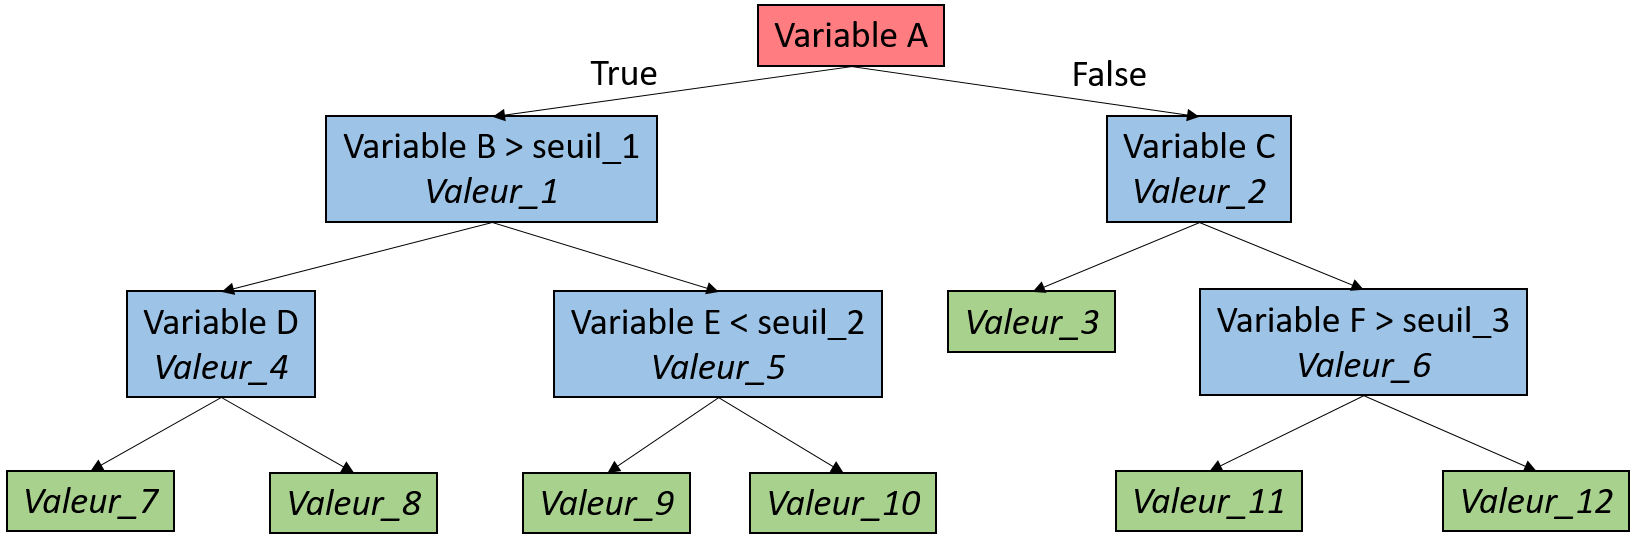
\includegraphics[width=1.0\linewidth]{figures/chapter-3/decision-tree-example} 
  \caption{Exemple schématique d'arbre de décision de régression. Le \textit{root node} est en rouge, les noeuds sont en bleu et les feuilles en vert. 
	Les variables A, C et D sont catégorielles ; les variables B, E et F sont numériques. Les "Valeurs\_X" correspondent à la valeur 
	prédite par l'arbre de décision de la variable dépendante suite à la division précédente.}
  \label{Figure:factors_decision_tree_example}
\end{figure}

Afin que les seuils calculés par le \gls{dt} aient un sens, la variables indépendantes n'ont ici pas été standardisées. Dans le cas de la \gls{saob}, 
les facteurs se retrouvent dans les noeuds : leur influence sur l'efficacité du \gls{nfb} est quantifiée par la valeur de la variable dépendante 
obtenue après chaque division mais aussi par leur place dans l'arbre. En effet, plus un facteur est en haut de l'arbre plus les divisions se font sur un grand nombre
d'observations, ainsi son impact sur l'efficacité est davantage probable.

\section{Analyse des facteurs influençant le Neurofeedback} %update avec dernière analyse

Les résultats de la \gls{saob} sont présentés ici. Cette méthode, dont les premières étapes (i.e. la sélection des études et le calcul des \gls{es}) rappellent
la méta-analyse, se distingue de cette dernière par l'utilisation de méthodes multivariées. Celles-ci tirent avantage de l'hétérogénéité des études
sur le \gls{nfb} appliqué aux enfants \gls{tdah} pour déterminer les facteurs ayant un impact sur la performance du \gls{nfb}.

\subsection{Sélection des études} \label{selection_studies}

Les termes entrés dans Pubmed pour la recherche des articles à inclure dans la \gls{saob} sont :
(ADHD OR adhd OR attention deficit disorder with hyperactivity OR minimal brain disorders OR syndrome hyperkinetic OR hyperkinetic
syndrome OR hyperactivity disorder OR hyperactive child syndrome OR childhood hyperkinetic syndrome OR attention deficit hyperactivity disorders
OR attention deficit hyperactivity disorder OR adhd attention deficit hyperactivity disorder OR addh OR overactive child syndrome OR attention deficit 
hyperkinetic disorder OR hyperkinetic disorder OR attention deficit disorder hyperactivity OR attention deficit disorders hyperactivity OR child 
attention deficit disorder OR hyperkinetic syndromes OR syndromes hyperkinetic OR hyperkinetic syndrome childhood) AND 
(randomized control trial OR RCT OR randomized control study OR Pilot Study OR Study OR Trial OR randomized trial) AND 
(neurofeedback OR “EEG biofeedback” OR neurotherapy OR SCP OR “slow cortical potentials” OR Theta Beta Ratio OR “TBR”). 

La dernière recherche effectuée le 12 février 2018 avec ces termes a retourné 155 résultats, auxquels se sont ajoutés 22 articles inclus dans les précédentes 
méta-analyses sur le \gls{nfb} appliqué aux enfants \gls{tdah} \citep{Arns2009, Sonuga-Barke2013, Micoulaud2014, Cortese2016, Catala2017}. Afin de sélectionner
les études à inclure dans la \gls{saob}, les 177 résultats ont été filtrés à l'aide du pipeline représenté à la 
Figure~\ref{Figure:factors_pipeline_selection_studies}. Au final $k$ = 33 études ont été retenues, qui correspondent par ailleurs au critère d'inclusion de
\citet{Cortese2016} sans les exigences sur les groupes contrôles. 

\newpage\
\begin{figure}[h!]
  \centering
	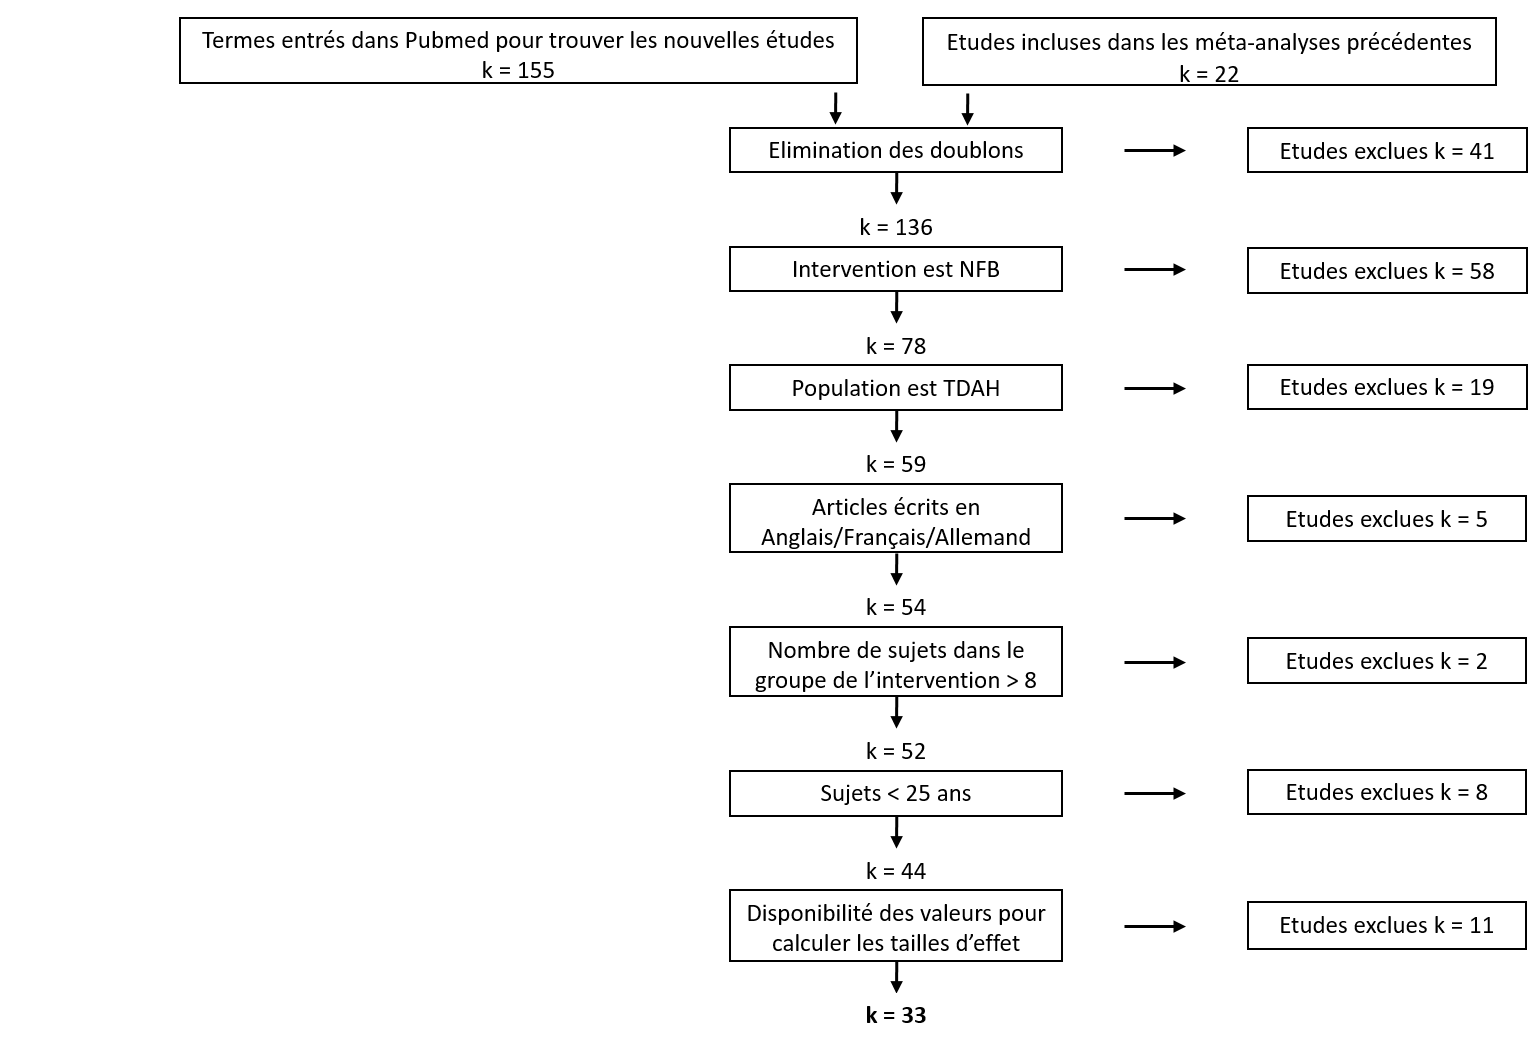
\includegraphics[width=1.0\linewidth]{figures/chapter-3/factors-selection-studies} 
  \caption{Diagramme de sélection des études pour l'analyse systématique des biais (dernière recherche le 12 fevrier 2018).} 
  \label{Figure:factors_pipeline_selection_studies}
\end{figure}

Les \gls{es}-intra-groupe sont calculés pour chaque étude puis les valeurs aberrantes sont rejetées comme expliqué en \ref{es_within}. 
La distribution des \gls{es}-intra-groupe ainsi que les bornes de l'intervalle d'inclusion sont représentées à la 
Figure~\ref{Figure:distribution_ES_within}. Les \gls{es}-intra-groupe négatifs sont en faveur du \gls{nfb}.

\begin{figure}[h!]
  \centering
	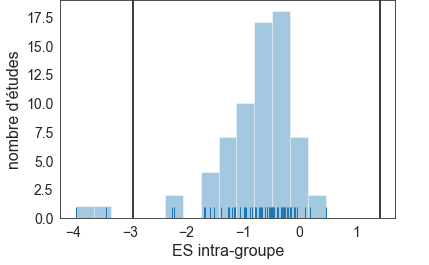
\includegraphics[width=0.5\linewidth]{figures/chapter-3/distribution-ES-within} 
  \caption{Distribution des tailles d'effet (\gls{es}) intra-groupe, une valeur négative est en faveur du Neurofeedback. Les lignes 
	verticales noires correspondent aux bornes supérieure et 
	inférieure de l'intervalle dans lequel les observations sont acceptées.}
  \label{Figure:distribution_ES_within}
\end{figure}

Sur la base de notre critère d'exclusion défini, $i = 3$ observations (3.40\%) issues de deux études (4.87\%): deux groupes de sujets de 
\citet{Bazanova2018} (celui de l'individualisation du \gls{nfb} et 
celui de l'individualisation du \gls{nfb} et du couplage avec \gls{emg}-Biofeedback) et les résultats obtenus avec les évaluations des 
parents de \citet{Rejabi2019}. 

En effet, ces trois observations présentent des \gls{es}-intra-groupe très larges, notamment les groupes de \citet{Bazanova2018} 
(respectivement -3.41 et -3.95). Ces \gls{es} extrêmement surprenants sont même plus élevés que ceux rapportés dans la littérature sur l'efficacité 
des psychostimulants sur les symptômes du \gls{tdah} chez les enfants \citep{Luan2017} comme illustré à la Figure~\ref{Figure:introduction-efficacy-treatments}. 
Ces valeurs invalident nos hypothèses de travail : dans le cas de la 
\gls{wls}, les résidus ne sont plus distribués normalement. Ainsi, afin de pouvoir conclure sur les résultats obtenus par la \gls{saob}, 
un rejet des valeurs aberrantes a été implémenté.

La \gls{saob} est donc effectuée sur 41 études (qui correspondent à 85 observations) évaluant l'efficacité du \gls{nfb} sur les enfants \gls{tdah} et 
qui sont listées dans la Table~\ref{Table:table_factors_analysis_meta_analysis_list_studies}. Au total, les 33 études sélectionnées rassemblent 
846 enfants \gls{tdah} effectuant du \gls{nfb}.

\newpage\
\begin{table}[h!]
  \centering
  \caption{Liste des études incluses dans l'analyse systématique des biais : a) études incluses dans \citet{Cortese2016}
	(dernière recherche le 30 août 2015) ; b) études satisfaisant le critère d'inclusion de \citet{Cortese2016} (dernière recherche le 12 février 2018) ; c) études 
	satisfaisant le critère d'inclusion de \citet{Cortese2016} à l'exception de la partie concernant le groupe contrôle (dernière recherche le 12 février 2018).}
  \fontsize{9}{11}\selectfont
\begin{tabular}{ cccccc }
\toprule
\multicolumn{3}{ c }{Analyse} & Etude & Année & \shortstack{ Nombre de sujets \\ dans le groupe \\ \gls{nfb} } \\
\midrule
 & & & \citeauthor{Arnold2014} & 2014 & 26 \\ 
 & & & \citeauthor{Bakhshayesh2011} & 2011 & 18 \\
 & & & \citeauthor{Beauregard2006} & 2006 & 15 \\
 & & & \citeauthor{Bink2014} & 2014 & 45 \\
 & & & \citeauthor{Christiansen2014} & 2014 & 14 \\
 & & & \citeauthor{Gevensleben2009} & 2009 & 59 \\
 & & & \citeauthor{Heinrich2004} & 2004 & 13 \\
 & & & \citeauthor{Holtmann2009} & 2009 & 20 \\
 & & & \citeauthor{Linden1996} & 1996 & 9 \\
 & & & \citeauthor{Maurizio2014} & 2014 & 13 \\
 & & & \citeauthor{Steiner2011} & 2011 & 9 \\
 & & & \citeauthor{Steiner2014} & 2014 & 34 \\
 & & & \citeauthor{VanDongen2013} & 2013 & 22 \\
 & & \shortstack{a = Réplication de \\ \citeauthor{Cortese2016}  \\ (voir \ref{replication}) } & \textbf{13 études} & & \textbf{297} \\
\cmidrule(lr){3-6}
 & & & \citeauthor{Aggensteiner2019} & 2019 & 75 \\
 & & & \citeauthor{Baumeister2016} & 2016 & 8 \\
 & & & \citeauthor{Bazanova2018} & 2018 & 17 \\
 & & & \citeauthor{Minder2018} & 2018 & 38 \\
 & & & \citeauthor{Moreno2019} & 2019 & 19 \\
 & & & \citeauthor{Strehl2017} & 2017 & 72 \\
 & & & \citeauthor{Shereena2019} & 2019 & 15 \\
 & \shortstack{b = Mise à jour \\ \citeauthor{Cortese2016} \\ (voir \ref{selection_studies}) } & & \textbf{16 études} & & \textbf{541} \\
\cmidrule(lr){2-6}
 & & & \citeauthor{Bluschke2016} & 2016 & 19 \\
 & & & \citeauthor{Cueli2019} & 2019 & 64 \\
 & & & \citeauthor{Deilami2016} & 2016 & 12 \\
 & & & \citeauthor{Drechsler2007} & 2007 & 17 \\
 & & & \citeauthor{Duric2012} & 2012 & 23 \\
 & & & \citeauthor{Escolano2014} & 2014 & 20 \\
 & & & \citeauthor{Fuchs2003} & 2003 & 22 \\
 & & & \citeauthor{Gelade2016} & 2016 & 39 \\
 & & & \citeauthor{Heinrich2019} & 2019 & 60 \\
 & & & \citeauthor{Kropotov2005} & 2005 & 86 \\
 & & & \citeauthor{Lee2017} & 2017 & 18 \\
 & & & \citeauthor{Leins2007} & 2007 & 19 \\
 & & & \citeauthor{Li2013} & 2013 & 32 \\
 & & & \citeauthor{Meisel2014} & 2014 & 12 \\
 & & & \citeauthor{Mohagheghi2017} & 2017 & 30 \\
 & & & \citeauthor{Mohammadi2015} & 2015 & 16 \\
 & & & \citeauthor{Monastra2002} & 2002 & 51 \\
 & & & \citeauthor{Ogrim2013} & 2013 & 13 \\
 & & & \citeauthor{Rajabi2019} & 2019 & 16 \\
 & & & \citeauthor{Sudnawa2018} & 2018 & 20 \\
 & & & \citeauthor{Strehl2006} & 2006 & 23 \\
 c = \gls{saob} & & & \textbf{41 études} & & \textbf{1 153} \\
\bottomrule
\end{tabular}

  \label{Table:table_factors_analysis_meta_analysis_list_studies}
\end{table}

\newpage\
\subsection{Facteurs identifiés méthode par méthode}

Vingt-huit paramètres ont été initialement identifiés afin d'analyser leur influence sur l'efficacité du \gls{nfb}. Parmi eux, neuf ont dû être exclus car ils étaient trop
homogènes ou présentaient trop d'observations manquantes : 
\begin{itemize}
	\item le protocole visant l'augmentation du rythme beta dans les aires frontales,
  \item l'utilisation d'une carte pour le transfert de l'entrainement à la maison et à l'école, 
  \item le type de seuillage pour les récompenses discrètes (incrémental ou fixe),
  \item la qualité de l'acquisition de l'\gls{eeg} égale à 3,
	\item la présence d'un groupe contrôle,
	\item l'individualisation des bandes de fréquences basée sur la valeur de l'\gls{iapf},
	\item le couplage entre le \gls{nfb} et l'\gls{emg}-Biofeedback qui demande au sujet de contrôler son activité cérébrale ene même temps que musculaire,
	\item la sévérité des symptômes du \gls{tdah},
	\item le degré d'engagement dans l'entraînement par \gls{nfb}.
\end{itemize} 

Afin de comparer la variabilité des valeurs au sein des facteurs non catégoriels sélectionnés, les boxplots des valeurs standardisées ont 
été obtenus et représentés à la Figure~\ref{Figure:factors-boxplots} :
\begin{figure}[h!]
  \centering
	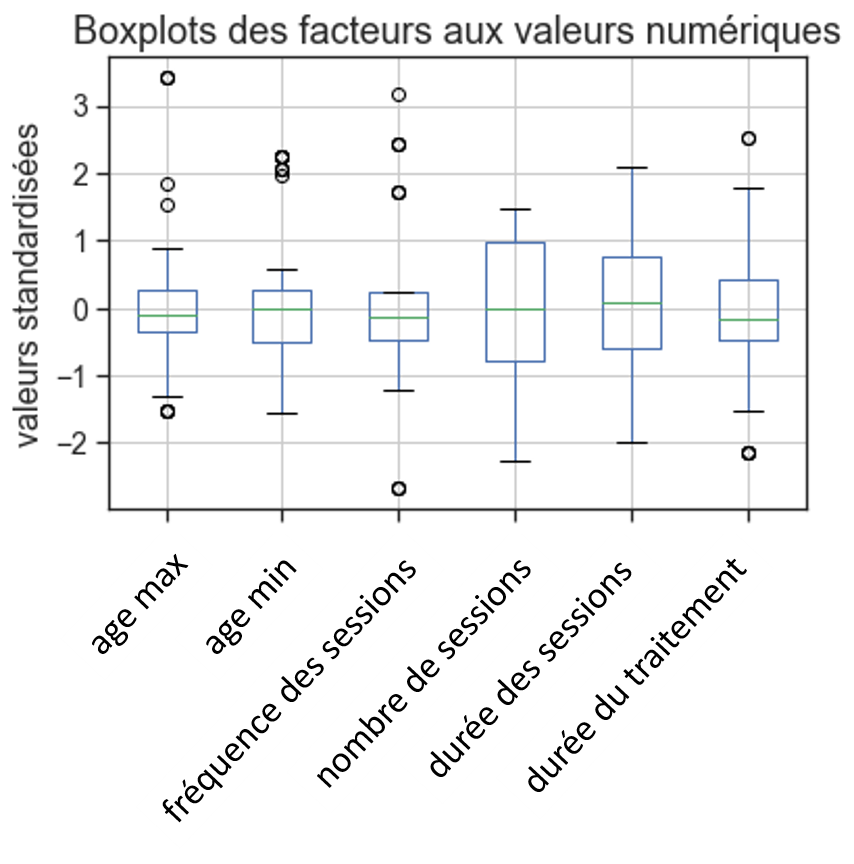
\includegraphics[width=0.7\linewidth]{figures/chapter-3/factors-distribution-of-factors} 
  \caption{Boxplots des facteurs aux valeurs numériques standardisées.} 
  \label{Figure:factors-boxplots}
\end{figure}

Le nombre de sessions et la durée de la session sont plus variables que l'âge minimal et maximal des enfants inclus dans l'étude. Les extrema et la 
moyenne de ces facteurs aux valeurs numériques non standardisées sont listés dans la Table~\ref{Table:table_factors_extremum_values} pour mettre en 
évidence la variabilité de ces facteurs dans les études incluses. 

\begin{table}[h!]
  \centering
  \caption{Extremum et moyenne des facteurs numériques non standardisés.}
  \fontsize{9}{11}\selectfont
\begin{tabular}{ cccc }
\toprule
Facteurs & Valeur minimale & Valeur maximale & Moyenne ($\pm$ std) \\
\midrule
Age max (en années) & 24 & 8.33 & 13.15 (3.16) \\
Age min (en années) & 5 & 12.33 & 8.00 (1.96) \\
Fréquence des sessions (par semaine) & 7 & 1 & 2.66 (1.37) \\
Nombre de sessions & 10 & 43 & 29.96 (8.78) \\
Durée de la session (en minutes) & 90 & 16 & 43.23 (22.42) \\
Durée du traitement (en semaines) & 30 & 3.0 & 13.17 (6.65) \\
\bottomrule
\end{tabular}
  \label{Table:table_factors_extremum_values}
\end{table}

Les trois méthodes décrites précédemment sont donc appliquées tour à tour sur les 19 facteurs restants. Tous les résultats sont résumés dans la 
Table~\ref{Table:table_factors_analysis_results_summary}.

\newpage\
\begin{table}[h!]
  \centering
  \caption{Resultats de la régression linéaire pondérée (\gls{wls}), de la régression linéaire régularisée (\gls{lasso}) et de l'arbre de décision (\gls{dt}). Pour la \gls{wls}, une p-value $<$ 0.05 
	(en gras) signifie que le coefficient du facteur correspondant est significativement différent de 0. Pour le \gls{lasso}, les facteurs dont les coefficients sont non mis à 0 (en gras) sont 
	sélectionnés. Pour l'arbre de décision, la place du facteur dans l'arbre est indiquée. Pour les deux premières colonnes, quand la valeur du coefficient est négative le facteur 
	correspondant pourrait mener à de meilleurs résultats du \gls{nfb}.}
  \begin{center}
\small 
\begin{tabular}{ p{3cm} p{3cm} p{3cm} p{2cm} p{2cm} p{2cm}}
\toprule
\multicolumn{2}{c}{ \shortstack{Variables \\ indépendantes (facteurs)} } & \shortstack{ Coefficients \\ trouvés par \gls{wls} \\ ($p$-value) } & \shortstack{ Coefficients \\ trouvés par \\ \gls{lasso} } & \shortstack{Place \\ sur le \\ \gls{dt}} \\
\midrule
\multirow{ 3}{*}{ \textit{Méthodologiques} } & \gls{pblind} & \hskip 0.12in\textbf{0.15 (0.015)} & \hskip 0.12in\textbf{0.086} & \textbf{\textit{root node}} \\ 
& randomisation & \hskip 0.12in0.013 (0.840) & \hskip 0.12in0.00 & / \\   
\midrule
\multirow{ 3}{*}{ \textit{Population} } & age max & \hskip 0.08in-0.10 (0.106) & \hskip 0.12in0.00 & / \\
& age min & \hskip 0.12in0.056 (0.43) & \hskip 0.12in0.00 & / \\
& prise de médicaments & \hskip 0.08in-0.026 (0.72) & \hskip 0.12in0.00 & / \\
\midrule
\multirow{ 9}{*}{ \textit{ \shortstack{Implementation \\ du \gls{nfb}} } } & nombre de sessions & \hskip 0.08in\textbf{-0.19 (0.025)} & \hskip 0.12in0.00 & / \\
& durée de la session & \hskip 0.08in-0.13 (0.16) & \hskip 0.12in0.00 & \textbf{2$^{eme}$ noeud} \\
& durée du traitement & \hskip 0.12in\textbf{0.39 (0.00)} & \hskip 0.12in\textbf{0.098} & \textbf{2$^{eme}$ et 3$^{eme}$ noeuds} \\
& fréquence des sessions & \hskip 0.12in0.027 (0.690) & \hskip 0.08in\textbf{-0.055} & \textbf{2$^{eme}$ noeud} \\ 
& \gls{smr} & \hskip 0.12in0.12 (0.067) & \hskip 0.12in0.00 & / \\
& augmentation de beta en central & \hskip 0.12in0.087 (0.32) & \hskip 0.12in\textbf{0.026} & / \\  
& diminution de theta & \hskip 0.08in-0.095 (0.39) & \hskip 0.12in0.00 & / \\
& \gls{scp} & \hskip 0.08in-0.14 (0.30) & \hskip 0.12in0.00 & / \\ 
& phase de transfert & \hskip 0.12in\textbf{0.33 (0.001)} & \hskip 0.12in\textbf{0.079} & \textbf{1$^{er}$ noeud} \\
\midrule
\multirow{ 2}{*}{ \textit{ \shortstack{Qualité de \\ l'acquisition} } } & plus d'une électrode d'enregistrement & \hskip 0.08in-0.083 (0.20) & \hskip 0.08in\textbf{-0.030} & / \\ 
& \gls{eeg} qualité 2 & \hskip 0.08in\textbf{-0.28 (0.00)} & \hskip 0.08in\textbf{-0.037} & / \\  
\midrule
\multirow{ 2}{*}{ \textit{Qualité du signal} } & rejet ou correction des artefacts oculaires & \hskip 0.08in-0.10 (0.164) & \hskip 0.08in\textbf{-0.0046} & \textbf{1$^{er}$ noeud} \\ 
& rejet des artefacts basé sur l'amplitude & \hskip 0.12in0.14 (0.058) & \hskip 0.12in0.00 & / \\   
\bottomrule
\end{tabular}
\end{center}

  \label{Table:table_factors_analysis_results_summary}
\end{table}

\subsubsection{La régression linéaire multiple et pondérée}

Les hypothèses de ce modèle sont respectées, les résultats sont interprétables :
\begin{itemize}
	\item la matrice ${\textbf{X}}^{T}\textbf{W}^{T}\textbf{WX}$ est bien régulière,
  \item aucune corrélation apparente n'est effectivement trouvée entre les variables indépendantes non catégorielles, 
  \item la tendance linéaire estimée est trouvée significative (Prob(F-statistic) = 7.58e-08),
  \item les résidus sont distribués normalement (kurtosis = 3.154 et Prob(Omnibus) = 0.392).
\end{itemize}

La \gls{wls} a trouvé 9 facteurs significatifs (deuxième colonne de la Table~\ref{Table:table_factors_analysis_results_summary}) avec un \textit{adjusted R Squared} de 0.62. 
Dans le cas de l'\gls{ols}, les mêmes facteurs ont été trouvés significatifs (à l'exception de la qualité de 
l'\gls{eeg} égal à 2 et de la présence de plus d'une électrode active) mais avec un \textit{adjusted R Squared} plus faible (0.35). Ainsi, associer un poids
à chaque observation permet d'expliquer davantage de variabilité. 

Il est important de noter qu'étant donné qu'un \gls{es}-intra-groupe négatif est en faveur de l'efficacité du \gls{nfb},
un facteur dont le coefficient est négatif aurait une influence positive sur les résultats \gls{nfb}.


\subsubsection{La régression linéaire régularisée}

La validation croisée \textit{leave-one-out} illustrée à la Figure~\ref{Figure:selection_lambda_lasso} a permis de déterminer un $\lambda$ optimal égal à 0.059.
\begin{figure}[h!]
  \centering
	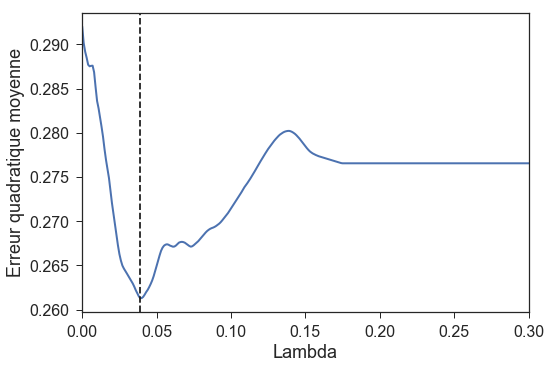
\includegraphics[width=0.5\linewidth]{figures/chapter-3/factors-selection-lasso-best-lambda} 
  \caption{Erreur quadratique moyenne (\gls{mse}) obtenue sur la moyenne de tous les \textit{folds} utilisés lors de la validation 
	croisée \textit{leave-one-out}. La courbe bleue représente la \gls{mse} moyennée sur tous les \textit{folds} ; la droite verticale en pointillé correspond
	au minimum de la \gls{mse} moyenne.}
  \label{Figure:selection_lambda_lasso}
\end{figure}

Le \gls{lasso} a gardé six facteurs différents de 0 (troisième colonne de la Table~\ref{Table:table_factors_analysis_results_summary}). Pour cette méthode également,
un facteur dont le coefficient est négatif aurait un bon impact sur l'efficacité du \gls{nfb}.

\subsubsection{L'arbre de décision de régression}

L'arbre de décision obtenu est présenté à la Figure~\ref{Figure:factors_decision_tree} : \gls{pblind} est le meilleur prédicteur (dernière colonne de la
Table~\ref{Table:table_factors_analysis_results_summary}). Quatre autres facteurs divisent ensuite les sous-ensembles, toutefois étant donné que de moins
en moins d'observations sont disponibles plus on descend dans l'arbre, l'influence de ces facteurs est de moins en moins certaine.

\begin{figure}[h!]
  \centering
	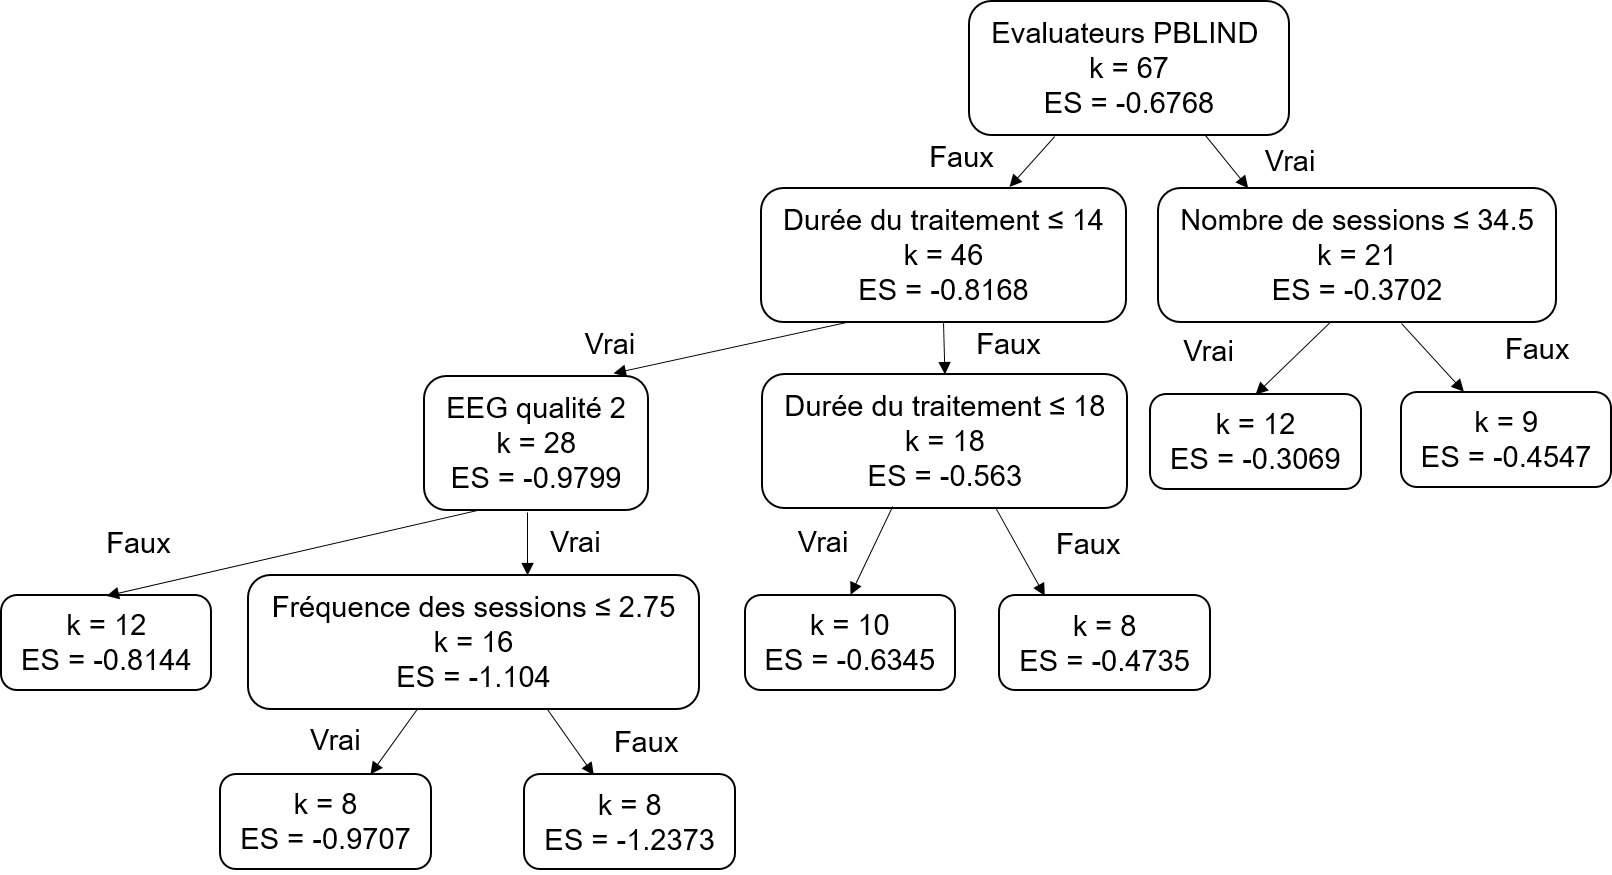
\includegraphics[width=1\linewidth]{figures/chapter-3/factors-decision-tree} 
  \caption{Arbre de décision obtenu : \gls{es} correspond à l'\gls{es}-intra-groupe et $k$ au nombre d'études. L'importance des variables indépendantes
	décroît depuis le \textit{root node}. La durée de la session est mesurée en minutes, la durée du traitement en semaines et l'âge en années.}
  \label{Figure:factors_decision_tree}
\end{figure}

\subsection{Résumé des résultats}

Plusieurs facteurs ont été trouvés significatifs par plus les trois méthodes : les évaluateurs \gls{pblind}, la qualité de l'\gls{eeg} égale à 2 et la durée du traitement. 
De plus, toutes les méthodes s'accordent quant à la direction de leur influence : alors qu'évaluer l'efficacité du \gls{nfb} en étant \gls{pblind}
semble conduire à de moins bons résultats, une durée de traitement plus courte et l'acquisition de l'\gls{eeg} avec un bon matériel mèneraient à un traitement plus efficace. 

L'influence des facteurs retournés par deux méthodes est plus incertaine :
\begin{itemize}
	\item la \gls{wls} et le \gls{lasso} trouvent tous deux qu'utiliser plus d'une électrode active durant la session de \gls{nfb} mènerait à de bons résultats,
  \item la \gls{wls} et le \gls{dt} conluent tous deux qu'effectuer un grand nombre de sessions est préférable, 
  \item le \gls{lasso} et le \gls{dt} obtiennent tous deux qu'un nombre élevé de sessions par semaine influencerait positivement les résultats. 
\end{itemize}

Cinq facteurs sont retournés seulement par une méthode : la randomisation des groupes, le recours à un \gls{irb}, la durée de la session, la présence d'une phase de transfert,
et la correction ou rejet des artefacts oculaires. 

Huit facteurs, n'ont quant à eux été sélectionnés par aucune méthode : l'âge minimum et maximum des enfants, prendre des 
médicaments pendant le traitement par \gls{nfb}, les protocoles \gls{smr}, augmentation de beta dans les aires centrales, diminution de theta et \gls{scp}, et la correction
des artefacts basée sur l'amplitude. Ainsi ces facteurs n'influenceraient pas l'efficacité du \gls{nfb}. 

Ces résultats sont résumés à la Table~\ref{Table:table_factors_analysis_results_summary_number_of_factors}.

\begin{table}[h!]
  \centering
  \caption{Facteurs classés selon le nombre de méthodes les identifiant comme significatifs. Un signe + signifie que la présence (dans le cas d'une variable catégorielle) ou l'importante valeur
	de la variable a un effet favorable sur l'efficacité du \gls{nfb}. A l'inverse, un signe - signifie que l'absence (dans le cas d'une variable catégorielle) ou la faible valeur
	de la variable a un effet favorable sur l'efficacité du \gls{nfb}. Le nombre de signes est décroissant avec le degré de confiance accordé à l'influence du facteur. 0 signifie 
	que le facteur n'aurait pas d'effet.}
  \begin{center}
\small 
\begin{tabular}{ ccc }
\toprule
\shortstack{Nombre de \\ méthodes}  & Facteurs & \shortstack{ Sens de \\ l'influence } \\
\midrule
\multirow{ 3}{*}{ \textit{3 méthodes} } & \gls{pblind} & - - - \\ 
& durée du traitement & - - - \\  
& phase de transfert & - - - \\  
\midrule
\multirow{ 3}{*}{ \textit{2 méthodes} } & \gls{eeg} qualité 2 & + + \\
& fréquence des sessions & + + \\
& \gls{eog} rejet ou correction & + + \\
\midrule
\multirow{ 5}{*}{ \textit{1 méthode} } & nombre de sessions & + \\
& durée de la session & - \\
& augmentation de beta en central & - \\
& plus d'une électrode d'enregistrement & + \\
\midrule
\multirow{ 8}{*}{ \textit{ Aucune méthode } } & randomisation & 0 \\ 
& age min & 0 \\ 
& age max & 0\\  
& prise de médicaments & 0 \\
& \gls{smr} & 0 \\
& diminution de theta & 0 \\
& \gls{scp} & 0 \\
& rejet des artefacts basé sur l'amplitude & 0 \\
\bottomrule
\end{tabular}
\end{center}
  \label{Table:table_factors_analysis_results_summary_number_of_factors}
\end{table}

\section{Discussion}

La description et l'analyse des différents types d'implémentation de \gls{nfb} ont fait l'objet de plusieurs études \citep{Arns2014, 
Jeunet2018, Arns2009, Cortese2016, Alkoby2017}. Cependant, à notre connaissance, aucune de ces études n'a implémenté une approche systématique et 
multivariée pour associer les facteurs aux résultats cliniques. La rigueur et la transparence lors de la conduite d'essais cliniques sur l'efficacité
du \gls{nfb} est essentielle pour comprendre son effet sur les fonctions cérébrales et le comportement comme le soulignent \citet{Ros2019} lors de l'élaboration
de leur liste de bonnes pratiques. 

\subsection{Facteurs et efficacité du \gls{nfb}}

La \gls{saob} a permis d'identifier des facteurs ayant une potentielle influence sur l'efficacité du \gls{nfb}. Certains facteurs ont été trouvés par les trois méthodes,
d'autres par deux ou une et certains par aucune. Ces résultats sont discutés ici, en s'intéressant à la fois aux paramètres pour lesquels l'influence sur la performance
clinique est fortement probable et à ceux pour lesquels l'impact s'avère moins certain. 

Comme attendu, le nombre de sessions s'avère être identifié par deux méthodes ce qui est en accord avec la littérature existante. En effet, grâce à plusieurs régressions linéaires 
simples sans correction pour tests multiples \citep{Arns2009}, \citet{Arns2014} affirme qu'effectuer moins de 20 sessions de \gls{nfb} conduit à une moins bonne efficacité. De même,
\citet{Vernon2004} a observé que des changements positifs, aussi bien sur l'\gls{eeg} qu'au niveau comportemental, apparaissent après au moins 20 sessions. Toutefois, \citep{Enriquez2017}
souligne le fait que le nombre de sessions doit être choisi avec précaution afin d'éviter "l'\textit{overtraining}". Le fait que le nombre de sessions n'a pas été identifié par le \gls{lasso}
pourrait s'expliquer par la présence de seulement deux observations de 20 sessions ou moins. Ainsi, étant donné que le seuil minimal pour obtenir des résultats avec l'entrainement
par \gls{nfb} semble dépassé pour la très grande majorité des observations, il est peu probable que ce facteur puisse être retrouvé par les trois méthodes sur cet ensemble de données. 
Toutefois, les deux méthodes qui ont identifié ce facteur s'accordent toutes deux sur la direction de l'effet : comme attendu plus le nombre de sessions effectué est important, 
plus le \gls{nfb} semble être efficace. 

Le type de protocole \gls{nfb} n'a été identifié par aucune méthode et donc n'influencerait pas l'efficacité du \gls{nfb}. Cette importance minime octroyée par la \gls{saob} au type de protocole
est contre-intuitive étant donné le rôle central du protocole choisi sur le mode d'action neurophysiologique et donc sur l'impact sur l'efficacité thérapeutique \citep{Vernon2004}. Une probable 
explication pour ce résultat est que tous ces protocoles ont une efficacité équivalente sur les populations étudiées et donc ne représentent pas un facteur explicatif significatif. 
Toutefois, ce résultat n'exclut pas une stratégie personnalisée basée sur les phénotypes pour augmenter les performances, comme précédemment suggéré par \citet{Alkoby2017}.

Trois facteurs ont été identifiés par les trois méthodes avec, de plus, la même direction d'influence : la qualité de l'\gls{eeg} égale à 2, la durée du traitement, et les évaluateurs 
probablement aveugles au traitement. 

Tout d'abord, la \gls{saob} a montré qu'enregistrer l'\gls{eeg} dans de bonnes conditions mène à de meilleurs résultats. Cette observation peut s'expliquer par le fait qu'un signal
\gls{eeg} de bonne qualité permet l'extraction plus précise des caractéristiques de l'\gls{eeg} liées au \gls{tdah} et donc conduit à un meilleur apprentissage et 
à une efficacité thérapeutique augmentée. Cependant, évaluer la qualité des moyens d'acquisition de l'\gls{eeg} (comme l'amplificateur utilisé) 
est difficile du fait du peu d'informations fourni par les études à ce sujet. Par conséquent, les futures essais cliniques devraient apporter plus 
de précisions quant au matériel utilisé afin de pouvoir plus aisément juger de sa qualité. La qualité d'acquisition de signaux \gls{eeg} peut être évaluée grâce à différentes
métriques dont certaines ont été utilisées par \citep{Bussalb2018benchmark} lors de la comparaison de différents systèmes \gls{eeg}. 

Ensuite, il semblerait que plus le traitement par \gls{nfb} est long, moins il devient efficace. Ce résultat semble contradictoire, à première vue, à la direction de l'effet donné
aux critères "nombre de sessions" et "fréquence des sessions". Le degré d'engagement dans l'intervention pourrait expliquer ce
résultat : être engagé dans un traitement long est plus compliqué. Cependant, il est difficile de quantifier ce degré car, soit aucun questionnaire n'est rempli 
par les enfants à ce sujet, soit cette information n'est pas mentionnée. 

Par ailleurs, la durée du traitement est étroitement liée à son intensité, ainsi on peut supposer qu'une période de traitement plus courte est préférable 
du fait de la fréquence plus élevée des sessions. Cette hypothèse est étayée par 
le fait que la variable "fréquence des sessions" (nombre de sessions par semaine) est aussi associée à de plus grands \gls{es}-intra-groupe selon le
\gls{lasso} et le \gls{dt}. L'impact de l'intensité du traitement par \gls{nfb} a été exploré par \citet{Rogala2016} sur des sujets adultes sains : il est
observé que les études proposant au moins 4 sessions de \gls{nfb} sur des jours consécutifs sont toutes bénéfiques. Par ailleurs, un autre facteur permet de soutenir
qu'un traitement intensif est favorable : le nombre de sessions lequel, selon la \gls{wls} et le \gls{dt}, semble plus favorable lorsqu'il 
est important. Ainsi, ces résultats indiquent qu'adopter une fréquence élevée de sessions est préférable, ce qui est peu connu dans le domaine du \gls{nfb}.

\subsection{Perspectives pour de futures analyses}

L'influence d'autres facteurs sur l'efficacité du \gls{nfb} aurait été intéressante à analyser, comme la personnalisation des protocoles d'entrainement basée sur l'\gls{iapf},
dont les résultats paraissent prometteurs selon \citet{Bazanova2018} et \citet{Escolano2014}. Cependant elle n'a pas pu être incluse dans la \gls{saob} faute d'un 
nombre suffisant d'études proposant un protocole personnalisé. Ce manque d'études est aussi la raison pour laquelle le couplage entre l'\gls{emg}-Biofeedback et le 
\gls{nfb} n'a pas pu être étudié dans la \gls{saob}. 

Un autre facteur intéressant, qui aurait pu aider à expliquer les résultats sur la durée du traitement, a 
également été exclu de l'analyse : la sévérité des symptômes à pré-test. Bien que les scores à pré-test soient disponibles pour chaque étude, ils ne sont pas
comparables car différentes échelles sont utilisées. Afin de résoudre ce problème, ces scores ont été normalisés grâce au score maximum pouvant être atteint
sur chaque échelle. Toutefois, cette valeur n'a pas pu être trouvée pour plusieurs échelles cliniques : trop d'observations manquantes ont mené au rejet de facteur.

Enfin, il serait intéressant de s'intéresser au lieu où les sessions de \gls{nfb} sont effectuées. En effet, \citet{Minder2018} souligne le fait que le lieu
d'entrainement pourrait aussi être un facteur contribuant à l'efficacité du \gls{nfb}. Toutefois, dans son étude aucune différence significative n'est trouvée entre
les résultats des performances à la clinique et à l'école. Dans la grande majorité des études sur le \gls{nfb} appliqué aux enfants
\gls{tdah}, les sessions ont lieu en clinique, rendant impossible à la \gls{saob} d'étudier ce facteur. Cependant, à l'instar de \citet{Minder2018}, d'autres 
études effectuent leurs séances en dehors du milieu hospitalier \citep{Bioulac2019}, ainsi l'influence du lieu d'entrainement pourra finir par être étudiée
plus précisément. Cela sera aussi valable pour les facteurs évoqués plus tôt et qui ont dû être exclus de la \gls{saob}.

\subsection{Analyse approfondie des évaluateurs probablement aveugles}

Les résultats de la \gls{saob} sont globalement en faveur de l'efficacité du \gls{nfb} pour le traitement des enfants \gls{tdah}, notamment l'utilisation 
de systèmes d'acquisition de bonne qualité et le rythme soutenu du traitement. Toutefois, comme attendu, l'évaluation
des symptômes par des personnes non-aveugles (\gls{mprox}) conduit à des résultats plus favorables que celles des évaluateurs \gls{pblind}, ce qui est en accord avec les
méta-analyses existantes \citep{Micoulaud2014, Cortese2016}. 

Les enseignants sont considérés comme \gls{pblind} par \citet{Cortese2016, Micoulaud2014} et cette définition a été suivie dans la \gls{saob}. Etonnamment, les données
à disposition ne vont pas exactement dans le sens de l'hypothèse largement acceptée que la différence entre \gls{mprox} et \gls{pblind} peut être seulement 
expliquée par l'effet placebo. Par ailleurs, les enseignants sont désignés comme "probablement" aveugles, ce qui signifie qu'ils peuvent être au courant du
traitement suivi par les enfants. En effet, il est possible que certains enseignants voient les enfants prendre des psychostimulants lors des pauses.
Cependant, il est difficile d'évaluer l'amplitude de ce phénomène. 

Un élément corrobore cette hypothèse : pour chaque étude incluse dans cette analyse, l'évaluation des symptômes avant le début
du traitement par les parents comparée à celle des enseignants montre que ces derniers ne voient pas l'ensemble des symptômes, autrement dit qu'ils sont probablement
plus aveugles aux symptômes qu'au traitement comme l'illustre la Figure~\ref{Figure:factors_pblind_discussion}. En effet, à pré-test, les enseignants évaluent les 
symptômes moins sévèrement que les parents et observent moins d'amélioration à post-test : cela correspond davantage au cas \textbf{A} représentant l'absence d'effet placebo
qu'au cas \textbf{B}.

\begin{figure}[h!]
  \centering
	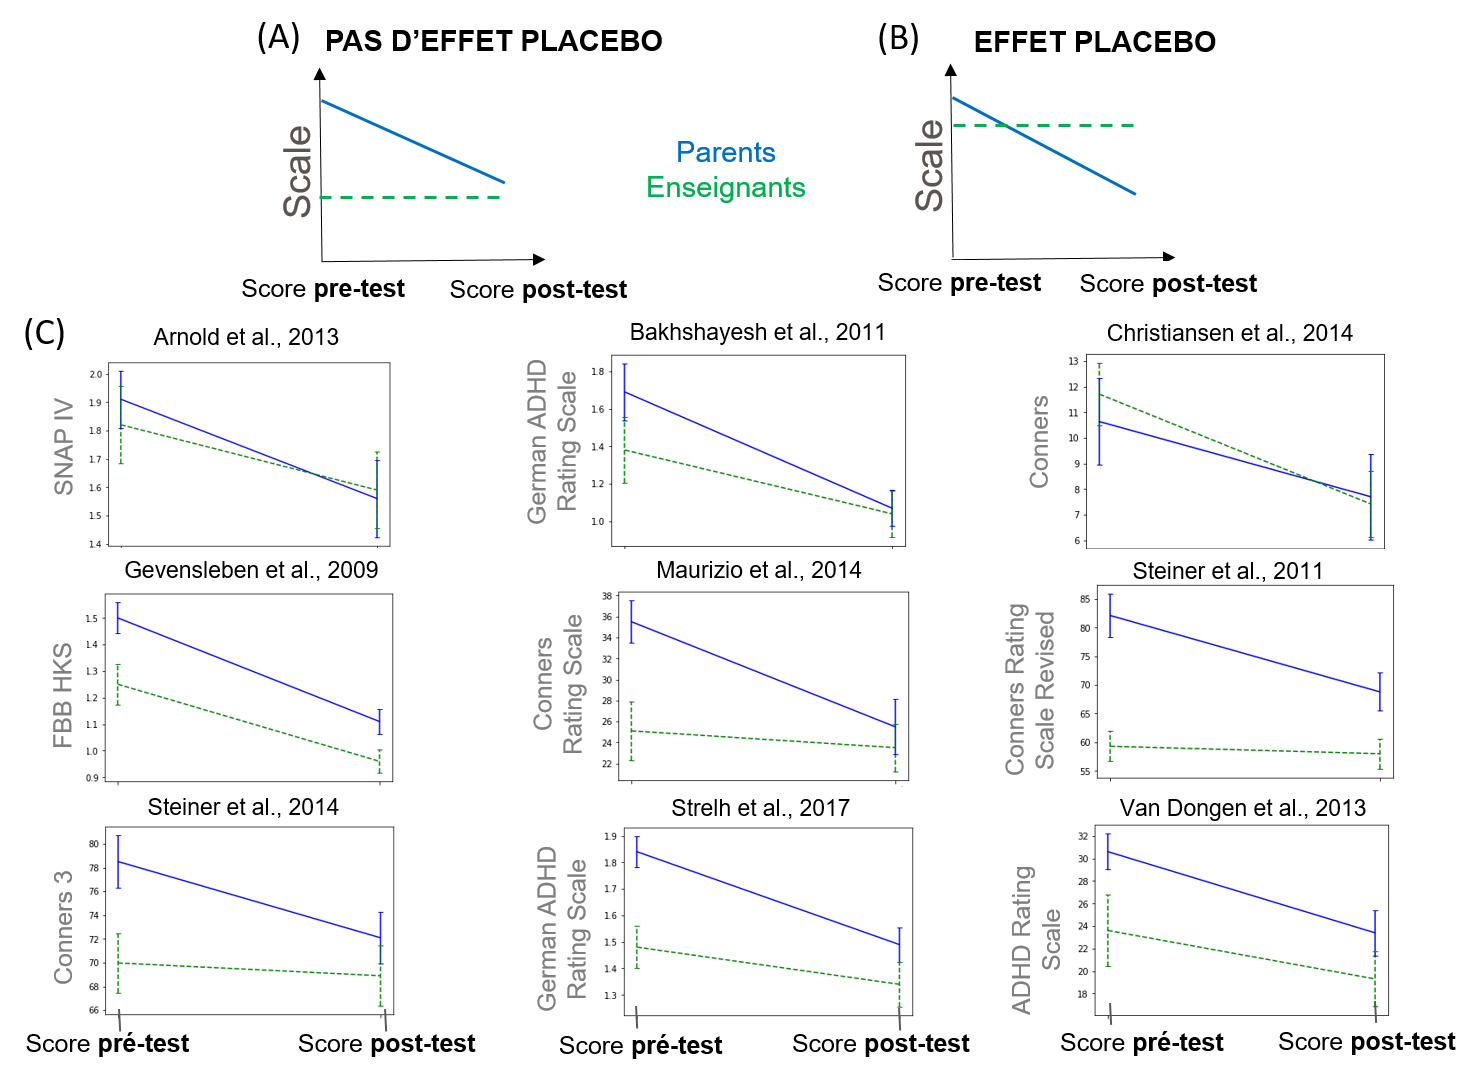
\includegraphics[width=1\linewidth]{figures/chapter-3/factors-pblind-discussion} 
  \caption{Scores à pré-test et post-test ($\pm$ erreur type) donnés par les parents (\gls{mprox}) en bleu et les enseignants (\gls{pblind}) en pointillés verts. 
	Deux hypothèses sur des données hypothétiques : \textbf{A)} pas d'effet placebo, les enseignants notent moins de symptômes du \gls{tdah} donc la difference entre pré et post-test est faible
	et \textbf{B)} effet placebo, les enseignants observent autant de symptômes à pré-test que les parents mais pas autant d'amélioration. \textbf{C)} Données réelles : 
	évolution des scores attribués par les parents et enseignants entre pré- et post-test dans les études qui satisfont le critère d'inclusion de \citeauthor{Cortese2016} 
	et qui donnent les scores sur les mêmes échelles pour les deux types d'évaluateurs.}
  \label{Figure:factors_pblind_discussion}
\end{figure}

Ces différences d'évaluation entre parents et enseignants ont été étudiées à de multiples reprises \citep{Sollie2013, Narad2015, Minder2018}, montrant que 
ces derniers sont plus susceptibles de sous-estimer la sévérité des symptômes du \gls{tdah} chez l'enfant, surtout chez les plus jeunes. Par conséquent, les 
enseignants sont peut-être simplement moins capables d'observer un changement clinique durant la durée du traitement. Par ailleurs, les scores entre enseignants 
sont plus variables que ceux entre parents, ce qui peut en partie expliquer le faible \gls{es} (aussi bien intra que inter-groupes) calculé pour les évaluateurs
\gls{pblind}. Ainsi pour conclure, recourir aux évaluateurs \gls{pblind} pour estimer l'effet placebo n'apparait pas comme étant un choix approprié. 

Une autre façon de mettre en évidence un éventuel effet placebo est de se rapporter au \gls{dt} présenté à la Figure~\ref{Figure:factors_decision_tree}. Le 
\textit{root node} divise l'ensemble des données en deux parties : d'une part un sous arbre est créé avec 46 observations correspondant aux évaluateurs
\gls{mprox} et d'autre part, 21 observations correspondant aux évaluateurs \gls{pblind}. Si les différences observées entre ces deux types d'évaluateurs est due à l'effet
placebo, il serait attendu que le sous-arbre des observations \gls{mprox} comporte des facteurs liés à la perception de l'implication dans le traitement. En effet, dans cette
partie de l'arbre on trouve bien le facteur "`durée du traitement", mais qui ne va pas dans la direction corroborant l'effet placebo : intuitivement, 
il est attendu que plus le traitement est long, plus l'effet placebo est important et plus l'\gls{es}-intra-groupe est élevé, or ici l'inverse est observé ce qui
contredit l'hypothèse. 

Ainsi, ces résultats suggèrent que les évaluateurs \gls{pblind} peuvent difficilement être utilisés pour quantifier l'effet placebo étant donné qu'ils paraissent
plus aveugles aux symptômes qu'au traitement. Etant donné que la mise en place de protocoles de \textit{sham}-\gls{nfb} éthiquement \citep{Holtmann2014} et techniquement 
\citep{Birbaumer1991} faisables est très difficile, il est nécessaire d'avoir recours à une méthode alternative et objective acceptable pour juger de l'efficacité du traitement 
\citep{World-Medical-Association2000}. Une analyse robuste envisageable serait d'étudier les neuromarqueurs collectés durant le traitement par \gls{nfb} pour démontrer que les 
patients contrôlent effectivement le neuromarqueur, qu'ils apprennent (c'est à dire que le contrôle du neuromarqueur s'intensifie avec le temps), et que cet apprentissage conduit 
à une réorgarnisation cérébrale durable. Ce genre d'analyse a été menée pour certaines études et conduit à des résultats favorables mais n'est pas 
systématique \citep{Arns2014}. Si aucune évolution du neuromarqueur n'est observée au cours du traitement alors que les évaluateurs \gls{mprox} notent une amélioration clinique 
des symptômes, on pourrait conclure que l'effet placebo joue un rôle dans ces résultats.

\subsection{Validation sur les nouvelles études publiées depuis le \\ 12/02/2018}

L'analyse précédente présente des résultats obtenus sur des études publiées avant le 12 février 2018 \citep{Bussalb2019clinical}, or la recherche dans le domaine 
du \gls{nfb} appliqué aux enfants \gls{tdah} est en pleine expansion conduisant à de nombreuses publications en peu de temps. 
Par ailleurs, plus le nombre d'études incluses dans la \gls{saob} sera important, plus ses résultats seront fiables. Par conséquent, une mise à jour 
est menée et ces nouveaux résultats sont comparés à ceux de \citet{Bussalb2019clinical}.

\subsubsection{Sélection des nouvelles études} 

Les résultats décrits précédemment ont été obtenus avec les études disponibles sur PubMed le 12 février 2018. Cependant, depuis cette date d'autres études satisfaisant
les critères d'inclusion présentés à la Figure~\ref{Figure:factors_pipeline_selection_studies} ont été publiées. Ainsi, la \gls{saob} a été mise à jour avec ces 
nouvelles études identifiées au 2 septembre 2019 dont les principales caractéristiques sont présentées dans la Table~\ref{Table:factors_new_studies_update}.

\begin{table}[h!]
  \centering
  \caption{Liste des études incluses dans l'analyse systématique des biais mise à jour par rapport à \citep{Bussalb2019clinical}: a) études satisfaisant le critère d'inclusion de \citet{Cortese2016} (dernière recherche 
	le 2 septembre 2019) ; c) études satisfaisant le critère d'inclusion de \citet{Cortese2016} à l'exception de la partie concernant le groupe contrôle 
	(dernière recherche le 2 septembre 2019).}
  \fontsize{9}{11}\selectfont
\begin{tabular}{ cccccc }
\toprule
\multicolumn{3}{ c }{Analyse} & Etude & Année & \shortstack{ Nombre de sujets \\ dans le groupe \\ Neurofeedback } \\
\midrule
 & & & \citeauthor{Aggensteiner2019} & 2019 & 75 \\
 & & & \citeauthor{Minder2018} & 2018 & 38 \\
 & & & \citeauthor{Moreno2019} & 2019 & 19 \\
 & & & \citeauthor{Shereena2019} & 2019 & 15 \\
 & \shortstack{a = Mise à jour \\ \citeauthor{Cortese2016} \\ (voir \ref{replication_and_update}) } & & 4 études & & 147 \\
\cmidrule(lr){2-6}
 & & & \citeauthor{Heinrich2019} & 2019 & 60 \\
 & & & \citeauthor{Rajabi2019} & 2019 & 16 \\
 & & & \citeauthor{Cueli2019} & 2019 & 64 \\
 & & & \citeauthor{Sudnawa2018} & 2018 & 20 \\
 b = Analyse \\ Systématique des \\bias & & & 8 études & & 160 \\
\bottomrule
\end{tabular}

  \label{Table:factors_new_studies_update}
\end{table}

Cette mise à jour permet ainsi d'appliquer la \gls{saob} sur 41 études ce qui correspond à 84 observations, augmentant ainsi la robustesse des
résultats. Malheureusement, tous les facteurs exclus dans l'analyse antérieure le sont également avec cette mise à jour et la validation par
un \gls{irb} est également rejetée.

\subsubsection{Résumé des résultats} 

Les hypothèses des méthodes utilisées dans la \gls{saob} sont validées, il est donc possible d'analyser les résultats qui sont présentés dans la 
Table~\ref{Table:table_factors_analysis_results_summary_update}.

\begin{table}[h!]
  \centering
  \caption{Resultats des mises à jour de la régression linéaire pondérée (\gls{wls}), de la régression linéaire régularisée (\gls{lasso}) et de l'arbre de décision (\gls{dt}). Pour la \gls{wls}, une p-value $<$ 0.05 
	(en gras) signifie que le coefficient du facteur correspondant est significativement différent de 0. Pour le \gls{lasso}, les facteurs dont les coefficients sont non mis à 0 (en gras) sont 
	sélectionnés. Pour l'arbre de décision, la place du facteur dans l'arbre est indiquée. Pour les deux premières colonnes, quand la valeur du coefficient est négative le facteur 
	correspondant pourrait mener à de meilleurs résultats du \gls{nfb}. Les valeurs en vert correspondent aux valeurs devenues significatives après la mise à jour ; les valeurs
	en rouges correspondent aux valeurs ayant perdu la significativité après la mise à jour.}
  \begin{center}
\small 
\begin{tabular}{ p{3cm} p{3cm} p{3cm} p{2cm} p{2cm} p{2cm}}
\toprule
\multicolumn{2}{c}{ \shortstack{Variables \\ indépendantes (facteurs)} } & \shortstack{ Coefficients \\ trouvés par \gls{wls} \\ ($p$-value) } & \shortstack{ Coefficients \\ trouvés par \\ \gls{lasso} } & \shortstack{Place \\ sur le \\ \gls{dt}} \\
\midrule
\multirow{ 3}{*}{ \textit{Méthodologiques} } & \gls{pblind} & \hskip 0.12in\textbf{0.15 (0.015)} & \hskip 0.12in\textbf{0.086} & \textbf{\textit{root node}} \\ 
& randomisation & \hskip 0.12in0.013 (0.840) & \hskip 0.12in\textcolor{red}{0.00} & / \\   
\midrule
\multirow{ 3}{*}{ \textit{Population} } & age max & \hskip 0.08in-0.10 (0.106) & \hskip 0.12in0.00 & / \\
& age min & \hskip 0.12in0.056 (0.43) & \hskip 0.12in0.00 & / \\
& prise de médicaments & \hskip 0.08in-0.026 (0.72) & \hskip 0.12in0.00 & / \\
\midrule
\multirow{ 9}{*}{ \textit{ \shortstack{Implementation \\ du \gls{nfb}} } } & nombre de sessions & \hskip 0.08in\textbf{-0.19 (0.025)} & \hskip 0.12in0.00 & \textcolor{red}{/} \\
& durée de la session & \hskip 0.08in\textcolor{red}{-0.13 (0.16)} & \hskip 0.12in0.00 & \textcolor{green}{\textbf{2$^{eme}$ noeud}} \\
& durée du traitement & \hskip 0.12in\textbf{0.39 (0.00)} & \hskip 0.12in\textbf{0.098} & \textbf{2$^{eme}$ et 3$^{eme}$ noeuds} \\
& fréquence des sessions & \hskip 0.12in0.027 (0.690) & \hskip 0.08in\textbf{-0.055} & \textbf{2$^{eme}$ noeud} \\ 
& \gls{smr} & \hskip 0.12in0.12 (0.067) & \hskip 0.12in0.00 & / \\
& augmentation de beta en central & \hskip 0.12in0.087 (0.32) & \hskip 0.12in\textcolor{green}{\textbf{0.026}} & / \\  
& diminution de theta & \hskip 0.08in-0.095 (0.39) & \hskip 0.12in0.00 & / \\
& \gls{scp} & \hskip 0.08in-0.14 (0.30) & \hskip 0.12in0.00 & / \\ 
& phase de transfert & \hskip 0.12in\textbf{0.33 (0.001)} & \hskip 0.12in\textcolor{green}{\textbf{0.079}} & \textcolor{green}{\textbf{1$^{er}$ noeud}} \\
\midrule
\multirow{ 2}{*}{ \textit{ \shortstack{Qualité de \\ l'acquisition} } } & plus d'une électrode d'enregistrement & \hskip 0.08in\textcolor{red}{-0.083 (0.20)} & \hskip 0.08in\textbf{-0.030} & / \\ 
& \gls{eeg} qualité 2 & \hskip 0.08in\textbf{-0.28 (0.00)} & \hskip 0.08in\textbf{-0.037} & \textcolor{red}{/} \\ 
\midrule
\multirow{ 2}{*}{ \textit{Qualité du signal} } & \gls{eog} rejet ou correction & \hskip 0.08in\textcolor{red}{-0.10 (0.164)} & \hskip 0.08in\textcolor{green}{\textbf{-0.0046}} & \textcolor{green}{\textbf{1$^{er}$ noeud}} \\ 
& Rejet des artefacts basé sur l'amplitude & \hskip 0.12in0.14 (0.058) & \hskip 0.12in0.00 & / \\   
\bottomrule
\end{tabular}
\end{center}
  \label{Table:table_factors_analysis_results_summary_update}
\end{table}

Les résultats obtenus sont globalement cohérents avec ceux présentés dans \citet{Bussalb2019clinical}. Alors que la \gls{wls} identifie les mêmes facteurs à l'exception de la correction ou rejet 
des artefacts oculaires (deuxième colonne de la Table~\ref{Table:table_factors_analysis_results_summary_update}), le \gls{lasso} (troisième colonne de la 
Table~\ref{Table:table_factors_analysis_results_summary_update}) est beaucoup plus sévère : tous les coefficients des facteurs sont mis à 0 sauf celui de \gls{pblind}. Ce facteur est ainsi 
le seul à être encore identifié par les trois méthodes qui s'accordent une nouvelle fois sur l'influence négative des évaluateurs aveugles sur les résultats.  

En ce qui concerne les deux autres facteurs précédemment identifiés par les trois méthodes : 
\begin{itemize}
\item la durée du traitement n'est plus retournée que par deux méthodes, 
\item la qualité de l'\gls{eeg} égale à 2 n'est plus retournée que par la \gls{wls}. 
\end{itemize}

Un seul autre facteur est identifié par deux méthodes : la présence d'une phase de transfert qui semblerait, selon la \gls{wls} et le \gls{dt}, avoir un impact négatif sur l'efficacité 
du \gls{nfb}. Ce facteur a été identifié dans \citet{Bussalb2019clinical} seulement par la \gls{wls} avec cette même direction d'effet.

\subsubsection{Discussion sur la mise à jour}

Entre le 12 février 2019 et le 2 septembre 2019, 8 nouvelles études répondant au critère d'inclusion de la \gls{saob} ont été publiées, ce qui montre l'importance de mettre à jour ce 
genre d'analyse. L'ajout de ces 8 études a modifié certaines conclusions de \citet{Bussalb2019clinical}. 

En effet, tout d'abord, la qualité de l'\gls{eeg} égale à 2 n'est plus retournée que par une seule méthode,
remettant en question son influence positive sur l'efficacité du \gls{nfb}. Toutefois, bien que ce facteur soit intéressant, sa définition, donnée en \ref{choix_des_facteurs}, manque de précision 
du fait du peu d'informations disponibles sur le matériel utilisé par les études. Ainsi, afin d'évaluer au mieux son influence, les études devraient fournir davantage d'informations. Ensuite, 
la durée du traitement n'est plus identifiée que par deux méthodes et la fréquence des sessions par une seule : on peut encore avancer, bien qu'avec moins de certitude que précédemment, 
qu'un traitement intensif est préférable. 

Alors que cette mise à jour a causé la perte de significativité de plusieurs facteurs, un facteur se voit identifié par deux méthodes : la présence d'une phase de transfert. 
Cette phase a pour but d'aider à transposer le contrôle appris lors des séances de \gls{nfb} à la vie de tous les jours, on pourrait donc s'attendre à un effet positif sur les symptômes
du \gls{tdah} comme le soulignent \citet{Arns2014, Strehl2006, Gani2008}, or la \gls{saob} conclut à un impact négatif. Ce résultat s'expliquerait peut-être par le fait qu'une phase de 
transfert seule ne soit pas si efficace si elle n'est pas couplée à l'utilisation d'une carte représentant la métaphore utilisée lors des sessions de \gls{nfb} qui permet à l'enfant de se 
souvenir plus facilement du contrôle qu'il exerçait durant la séance \citep{Bioulac2019, Bluschke2016}. Ce facteur devait être analysé mais étant trop homogène (plus de 80\% des observations 
n'utilisent pas de carte), il a été exclus de l'analyse. 

Bien que la significativité avait été atteinte pour la qualité de l'\gls{eeg} égale à 2 et pour la durée du traitement par les trois méthodes \citep{Bussalb2019clinical}, 
les résultats ne sont pas figés : ils vont fluctuer jusqu'à se stabiliser quand un grand nombre d'observations sera disponible. Ce constat est illustré dans le cadre de la méta-analyse 
présentée au chapitre \ref{chapitre-2} à la Figure~\ref{Figure:meta_analysis_evolution_pvalue}).

Ainsi, pour que la \gls{saob} puisse apporter des indications fiables quant au design d'une étude évaluant l'efficacité du \gls{nfb} appliqué aux enfants \gls{tdah}, elle doit être 
régulièrement mise à jour. 

\section{Conclusion}

La \gls{saob} a permis d'identifier un facteur lié au matériel d'acquisition de l'\gls{eeg} comme ayant une influence positive sur l'efficacité du \gls{nfb}, 
ce qui indique fortement qu'elle est liée à un mécanisme d'action basé sur la modulation de l'\gls{eeg}. Toutefois, la mise à jour de la \gls{saob} a rendu
plus incertain l'impact de ce paramètre dont la définition souffre du peu d'informations fourni par les études à ce sujet. Toutefois, étant donné que la
communauté du \gls{nfb} appelle à être le plus transparent possible quant au matériel utilisé \citep{Ros2019}, il sera sans doute possible d'étudier plus précisément
son impact lors de futures analyses.

L'intensité du traitement a aussi été trouvée comme contribuant à l'efficacité du \gls{nfb}, ce qui va dans le sens de ce qui est connu à propos de 
la théorie de l'apprentissage \citep{Mowrer1960} : un entrainement plus intense mène à une efficacité clinique augmentée. 

Alors que ces résultats contribuent certainement au débat, ce travail montre également que l'ultime démonstration de la preuve de l'efficacité du \gls{nfb}
appliqué aux enfants \gls{tdah} n'est pas encore atteinte, étant donné que les évaluations des enseignants ont été en partie invalidées comme indicatrices de 
l'effet placebo. Par conséquent, se référer aux résultats des évaluateurs \gls{pblind} pour mettre en évidence la spécificité de l'efficacité clinique n'est pas 
recommandé : il serait préférable d'avoir recours au sham-\gls{nfb} et à l'analyse des changements de l'\gls{eeg} en fonction des neuromarqueurs entrainés.

Comme l'a montré la mise à jour des résultats de la \gls{saob}, les conclusions de cette analyse peuvent encore évoluer. Au vu du nombre important 
d'études publiées sur le \gls{nfb} appliqué aux enfants \gls{tdah}, certains facteurs vont pouvoir finir par être inclus dans la \gls{saob}, comme par exemple 
l'individualisation du protocole de \gls{nfb} qui semble prometteuse. Le chapitre suivant va justement s'intéresser à la distribution d'un marqueur de l'attention, 
le \gls{tbr}, au sein d'une large population afin de déterminer si une personnalisation basée sur ce neuromarqueur est envisageable.




 

\newpage
\chapter{Analyse de la distribution d'un marqueur de l'attention au sein d'une population d'enfants TDAH}

\section*{Introduction}
Le \gls{tbr} a été massivment étudié chez les enfants \gls{tdah}. Diminuer le \gls{tbr} est par ailleurs un protocole d'entrainement de \gls{nfb} couramment utilisé 
pour traiter le \gls{tdah} chez les enfants \citep{Arnold2014, Deilami2016, Gevensleben2009, VanDongen2013}. Cependant, ce protocole ne serait peut-être pas adapté à tous les enfants \gls{tdah} si 
on se base sur le phénotype de leur \gls{eeg}. En effet, il a été avancé qu'il existerait un groupe d'enfants \gls{tdah} présentant un \gls{tbr} élevé 
\citep{Zhang2017, Clarke2011}, ainsi ces enfants bénéficieraient peut-être davantage d'un protocole diminuant leur \gls{tbr} que les autres. 

Quelques études ont proposé de personnaliser le protocole d'entrainement par \gls{nfb} \citep{Bazanova2018, Escolano2014}, mais trop peu pour en déterminer
l'impact sur l'efficacité du \gls{nfb} par la \gls{saob}. L'analyse présentée dans ce chapitre n'a pas pour but d'évaluer directement l'efficacité de la 
personnalisation des protocoles de \gls{nfb} mais sa pertinence. Pour ce faire, la distribution des valeurs de \gls{tbr} chez les enfants \gls{tdah} est 
étudiée à l'aide de différentes méthodes de partitionnement pour déterminer combien de groupes d'enfants \gls{tdah} existent en se basant seulement sur les 
valeurs de \gls{tbr}. 

\section{Population étudiée}

Les données utilisées dans cette analyse proviennent de trois bases de données différentes :
\begin{itemize}
\item NEWROFEED (NCT02778360, Mensia Technologies, France, ClinicalTrials.gov, \citet{Bioulac2019}),
\item \gls{cmi-mipdb} \citep{Langer2017, Langer2017b},
\item \gls{cmi-hbn} \citep{Alexander2017, Alexander2017b}.
\end{itemize}
Pour chacune de ces bases de données, un consentement éclairé écrit a été obtenu de tous les participants ou de leurs responsables légaux. Tous les enregistrements
ont été effectués dans un environnement contrôlé avec les yeux ouverts (\gls{eo} en anglais) et au repos (c'est à dire que le sujet n'effectue aucune tâche) 
pendant une minute sous la supervision d'un clinicien ou d'un chercheur. 

La description de l'ensemble des données est disponible dans la Table~\ref{Table:tbr_datasets_description}.

\begin{table}[h!]
  \centering
  \caption{Informations sur les données utilisées. Le critère d'inclusion pour chaque base de données est précisé, ainsi que le nombre de sujets satisfaisant
	chaque critère entre parenthèses. Le nombre total de sujets inclus par base de données est donné à la dernère ligne.}
  \fontsize{9}{11}\selectfont
\begin{tabular}{ ccccc }
\toprule
Base de données & NEWROFEED & CMI-MIPDB & \multicolumn{2}{ c }{CMI-HBN} \\
\midrule
\shortstack{ Description \\ de la population } & \shortstack{ - 7-13 ans \\ - Diagnostiqué \gls{tdah} \\ - Enregistré avec \\ l'appareil
                                               \\ Mensia Koala\textregistered : \\ 8 électrodes \\ du système 10-20 } 
																							 & \shortstack{ - 6-44 ans \\ - Avec et sans \\ diagnostic \\ - Enregistré avec \\ le système
                                               \gls{eeg} \\ Geodesic Hydrocel : \\ 128 électrodes } 
																							 & \multicolumn{2}{ c }{ \shortstack{ - 5-21 ans \\ - Avec et sans \\ diagnostic \\ - Enregistré avec \\ le système
                                               \gls{eeg} \\ Geodesic Hydrocel : \\ 128 électrodes } }
																							\\
\midrule
Nombre de sujets & \shortstack{ 122 (données disponibles \\ au 09/2017 pour les \\ analyses de contrôle \\ de la qualité avant \\ la fin de l'étude \\ en 12/2017) } 
                 & 126 
								 & \multicolumn{2}{ c }{ 881 }
								\\
\midrule
\shortstack{ Critères d'inclusion \\ additionnels} & \shortstack{ 1. Age/diagnostic \\ précisés (122) \\ 2. \textbf{Diagnostic} \\ \textbf{ \gls{tdah} } (122) \\ 3. \gls{eeg} d'une \\ min \gls{eo} 
                 au repos \\ disponible et \\ possible à \\ analyser (122) } 
                 & \shortstack{ 1. Age/diagnostic \\ précisés (126) \\ 2. \textbf{Diagnostic :} \\ \textbf{ \gls{tdah} } (12) \\ 3. \gls{eeg} d'une \\ min \gls{eo} 
                 au repos \\ disponible et \\ possible à \\ analyser (10) } 
								 & \shortstack{ 1. Age/diagnostic \\ précisés (447) \\ 2. \textbf{Diagnostic :} \\ \textbf{ \gls{tdah} } (237) \\ 3. \gls{eeg} d'une \\ min \gls{eo} 
                 au repos \\ disponible et \\ possible à \\ analyser (231) } 
								 & \shortstack{ 1. Age/diagnostic \\ précisés (447) \\ 2. \textbf{Diagnostic :} \\ \textbf{ Aucun }  (76) \\ 3. \gls{eeg} d'une \\ min \gls{eo}  
                 au repos \\disponible et \\ possible à \\ analyser (74) } 
								\\
\midrule
\shortstack{ Nombre de \\ sujets inclus} & 122 & 10 & 231 & 74 \\
\bottomrule
\end{tabular}
  \label{Table:tbr_datasets_description}
\end{table}

\subsection{Données NEWROFEED}

Une partie des données utilisées dans cette analyse provient de l'étude NEWROFEED (NCT02778360, Mensia Technologies, France, ClinicalTrials.gov, \citet{Bioulac2019})
qui avait pour but d'évaluer l'efficacité du \gls{nfb} à la maison versus celle du méthylphenidate sur une population d'enfants \gls{tdah}.
Au moment où le travail décrit dans ce chapitre a été mené, NEWROFEED était en cours donc 
seulement une partie des données était disponible. Ainsi, 122 enregistrements \gls{eeg} d'enfants diagnostiqués \gls{tdah} d'après les critères du DSM-IV \citep{DSM-4} 
ont été analysés. L'\gls{eeg} a été enregistré avec l'appareil Mensia Koala équipé de 8 électrodes \gls{agcl} individuellement blindées, positionnées sur le scalp suivant
le système international 10-20 : Fpz, F3, Fz, F4, C3, Cz, C4, Pz. La fréquence d'échantillonnage était de 512Hz. Les impédances devaient être
inférieures à $40$k$\Omega$ et le niveau de contamination électromagnétique devait rester inférieur à 1/3 de l'énergie totale du signal. 

Pour participer à l'étude NEWROFEED, les sujets devaient remplir les critères suivants :
\begin{itemize}
\item être des enfants ou adolescents (fille ou garçon) entre 7 et 13 ans,
\item avoir un diagnostic \gls{tdah} positif avec Kiddie-SADS \citep{Kaufman1997},
\item avoir un score sur l'ADHD RS IV supérieur à 6 pour l'inattention, avec ou sans hyperactivité \citep{Pappas2006}.
\end{itemize}

De plus, les enfants correspondant à un de ces critères ont été exclus :
\begin{itemize}
\item être \gls{tdah} avec le sous-type hyperactif/impulsif mais sans la composante inattention,
\item avoir un trouble psychiatrique sevère et/ou incontrôlable autre que le \gls{tdah} diagnostiqué avec Kiddie-SADS tel que par 
exemple l'autisme ou la schizophrénie,
\item avoir un trouble comorbide nécessitant des médicaments psychoactifs autres que ceux prescrits pour le \gls{tdah},
\item avoir un QI < 80 d'après les trois sous-tests du WASI ou du WISC \citep{Wechsler1999}.
\end{itemize}

Seule la première évaluation de l'\gls{eeg} enregistrée pour chaque patient avant le début du traitement par \gls{nfb} est utilisée pour cette analyse. 
L'étude NEWROFEED a été menée dans 12 centres cliniques dans 5 pays européens (France, Espagne, Allemagne, Belgique et Suisse).

\subsection{Données CMI-MIPDB}
Au moment de l'analyse, l'intégralité de la base \gls{cmi-mipdb} compte 126 participants à la fois avec et sans diagnostic clinique \citep{Langer2017, Langer2017b}.
Les participants ont été recrutés au Child Mind Medical Practice et dans la région de la ville de New-York. Chaque sujet a été questionné pendant 10 minutes
au téléphone ou en personne par un chercheur expérimenté pour évaluer son éligibilité grâce à :
\begin{itemize}
\item l'historique de ses troubles psychiatriques, incluant les traitements en cours et précédents,
\item l'historique de ses troubles neurologiques et/ou épilepsie.
\end{itemize}

L'enregistrement de l'\gls{eeg} est prévu si aucune contre indication n'est trouvée. 

De tous les patients présents dans la base \gls{cmi-mipdb}, seulement ceux satisfaisant les critères suivants ont été inclus dans l'analyse présentée dans ce chapitre :
\begin{enumerate}
\item être diagnostiqué\gls{tdah},
\item posséder un \gls{eeg} au repos disponible au format ".raw",
\item avoir son âge précisé.
\end{enumerate}

L'\gls{eeg} a été enregistré avec un système \gls{eeg} Geodesic Hydrocel à une fréquence d'échantillonnage de 500Hz et un filtre passe-bande entre 0.1 et 100Hz. 
L'électrode de référence est Cz, localisée au vertex de la tête. Le tour de tête de chaque participant est mesuré pour que le bonnet utilisé lors de l'enregistrement 
soit à la bonne taille. L'impédance des électrodes est gardée inférieure à $40$k$\Omega$ : elle est vérifiée toutes les 30 minutes ainsi qu'avant chaque enregitrement.

\subsection{Données CMI-HBN}
La base de données \gls{cmi-hbn} est composée de 881 sujets, avec ou sans diagnostic \citep{Alexander2017, Alexander2017b}. Les familles recoivent 150\$ pour leur participation 
et les sujets se voient de plus offrir les rapports de consultation et les avis sur les sessions d'\gls{eeg}.

Seuls les sujets remplissant les critères suivants ont été inclus dans notre analyse :
\begin{enumerate}
\item être diagnostiqué \gls{tdah} selon le KSADS-COMP \citep{Kaufman1997},
\item posséder un \gls{eeg} au repos disponible au format matlab ".mat",
\item avoir son âge précisé.
\end{enumerate}

Des 881 sujets disponibles, 231 (âgés entre 5 et 21 ans) satisfont ces critères et sont inclus dans notre analyse.

La base de données \gls{cmi-hbn} contient également des sujets sains qui vont être utilisés en tant qu'\textit{a priori} (\textit{priors} en anglais) pour le
modèle bayesien décrit en \label{clustering}. Pour être inclus dans cette analyse en tant que \textit{priors}, les sujets ne doivent avoir aucun diagnostic 
et doivent remplir les critères 2. et 3. cités précédemment. Au final, 74 sujets entre 5 et 21 ans sont sélectionnés. 

\subsection{Pré-traitement et homogénéisation des bases de données} \label{pré-traitement TBR}
Les \gls{eeg} des différentes bases de données sont pré-traités de façon à être comparables, notamment au niveau du placement des électrodes.
En ce qui concerne le traitement des artefacts et l'extraction du \gls{tbr}, les étapes sont les mêmes quelle que soit la base de données. 
Les pré-traitements ainsi que les analyses des signaux \gls{eeg} qui suivent sont effectués à l'aide du logiciel NeuroRT (v3, Mensia Technologies, 
Paris, France).

\subsubsection{Base de données NEWROFEED}
Le seul pré-traitement que nécessitent les signaux de la base de données NEWROFEED est un filtrage temporel : 
\begin{itemize}
\item un filtre Butterworth passe-haut d'ordre 1 à 0.5Hz afin d'enlever la composante continue (\textit{DC component} en anglais),
\item un filtre Butteroworth coupe-bande d'ordre 3 de 47 à 53Hz afin d'enlever l'artefact causé par les lignes électriques.
\end{itemize}

\subsubsection{Bases de données CMI}

Le pré-traitement des bases de données \gls{cmi-mipdb} et \gls{cmi-hbn} demande plus d'étapes : filtrage temporel, suppression et 
interpolation des canaux bruités et/ou déconnectés, et une interpolation spatiale afin de passer d'un espace à 128 électrodes \gls{egi},
à l'espace de 8 électrodes placées selon le système 10-20 utilisé dans la base de données NEWROFEED.

Tout d'abord, les \gls{eeg} obtenus au repos sont séparés en deux fichiers : l'un pour les enregistrements les yeux fermés, 
l'autre pour les enregistrements \gls{eo} ; seul ce dernier va être analysé. Ensuite, les mêmes filtres temporels vont être appliqués
que pour les données NEWROFEED, à l'exception du filtre coupe bande dont les bornes sont modifiées pour intercepter les artefacts 
causés par les lignes électriques américaines (57-63Hz).

Dans le cas d'enregistrements d'\gls{eeg} avec une haute résolution spatiale comme ici avec les données CMI, 
il est courant qu'au moins un canal se déconnecte ponctuellement causant aussi bien des artefacts de large amplitude que des signaux plats. 
Une strategie est ici mise en place pour détecter de façon fiable puis interpoler ces électrodes déconnectées. La variance de chaque canal 
\gls{eeg} est calculée sur une fenêtre glissante de 10 secondes. Cette variance est ensuite convertie en deux z-scores grâce à :
\begin{enumerate}
\item la distribution instantanée des variances pour les 127 autres canaux (z-score spatial),
\item la distribution cumulative des variances pour le canal d'intérêt (z-score temporel).
\end{enumerate}
Si le z-score temporel n'est pas compris entre -5 et 5, le signal est détecté comme étant un artefact et est interpolé à partir des canaux voisins.
Si le z-score spatial n'est pas compris entre -2 et 2, soit le signal a une trop grande variance (autrement dit il est bruité), soit une trop faible
variance (autrement dit l'électrode doit être déconnectée et n'energistre rien) : dans les deux cas il est interpolé.

Les données sont re-référéncées sur l'électrode de la mastoïde gauche (électrode 57 de l'\gls{egi}-128) pour correspondre au référencement de la base
de données NEWROFEED. Les signaux \gls{eeg} des 128 électrodes de l'espace \gls{egi} sont ensuite spatialement reconstruits dans l'espace à 8 électrodes 
dans le système international 10-20 en projetant les coordonnées sur une sphère unitaire.


\section{Theta-Beta ratio : un marqueur de l'attention}

\subsection{Définition du Theta-Beta ratio}
La littérature indique qu'il existerait différents groupes de patients \gls{tdah} identifiés à l'aide de leur profil \gls{eeg}, comme l'augmentation
de la puisssance dans la bande theta et/ou la diminution de la puissance dans la bande beta \citep{Clarke2011, Loo2018}. Ces différences de puissances dans ces 
bandes de fréquence peuvent être quantifiées en calculant la ratio de la puissance dans la bande theta et de la puissance dans la bande beta : le 
\gls{tbr} \citep{Arns2013}. 

De nombreuses études ont été menées pour analyser la pertinence d'utilser le \gls{tbr} comme biomarqueur pour diagnostiquer le \gls{tdah}. En effet, certains auteurs suggèrent qu'un \gls{tbr}
élevé peut aider à confirmer les diagnostics du \gls{tdah} \citep{NebaHealth, Saad2018, FDA}. Cependant, les études récentes ont échoué à repliquer les résultats
montrant une différence entre les valeurs de \gls{tbr} des patients \gls{tdah} et celles des patients sains, remettant en question son utilisation comme outil 
diagnostic \citep{Zhang2017, Arns2013, Clarke2001}. A la place, ces études trouvent qu'environ 35\% des sujets \gls{tdah} présenteraient un \gls{tbr} élevé : ce
résultat pourrait être utilisé pour identifier de meilleurs répondeurs à une intervention donnée. 

La diminution du \gls{tbr} fait partie des protocoles le plus couramment utilisé en \gls{nfb} appliqué aux enfants \gls{tdah} \citep{Arns2014}. 
On peut soutenir que l'efficacité de ce traitement pourrait être augmentée en affectant chaque patient à l'entraînement qui correspond le mieux à son phénotype \gls{eeg}. 
Par exemple, les sujets présentant un haut \gls{tbr} suivraient un protocole de \gls{nfb} où il est demandé de diminuer le \gls{tbr}. Cette répartition a été proposée lors 
de l'essai clinique NEWROFEED, pour lequel un seuil de répartition a dû être choisi. Un essai clinique randomisé et en double aveugle proposé par \citet{Kerson2013} 
prévoyait d'utiliser un seuil \gls{tbr} de 5 mais cette valeur a été modifiée et fixée à 4.5 (NCT02251743, Arnold, Ohio State University, ClinicalTrials.gov), valeur également
utilisée dans NEWROFEED. Choisir correctement la valeur de seuil est crucial car cette valeur détermine quel protocole \gls{nfb} le patient va suivre. 

Le caractère arbitraire des valeurs de seuil basées sur le \gls{tbr} et l'hétérogénéité des méthodes utilisées appelle à une validation précise de l'existence d'un 
sous-groupe de patients \gls{tdah} présentant un \gls{tbr} élevé, et de la valeur du seuil qui sépare ces sous-groupes. L'existence de deux sous-groupes \gls{tdah} distincts, 
définis par des valeurs faibles ou élevées doit être validée, tout comme le seuil à partir duquel les valeurs de \gls{tbr} sont considérées comme élevées.  
 

\subsection{Extraction du Theta-Beta ratio}
L'extraction du \gls{tbr} des \gls{eeg} pré-traités après \ref{pré-traitement TBR} comprend plusieurs étapes :
\begin{enumerate}
\item le rejet des artefacts en utilisant la géométrie Riemannienne,
\item l'extraction de l'\gls{iapf},
\item le calcul du \gls{tbr}.
\end{enumerate}

\subsubsection{Rejet des artefacts}
Tout d'abord, les données artefactées sont exclues en utilisant le \gls{rpf} \citep{Barthelemy2019}. Les données \gls{eeg} sont épochées (durée de 2 secondes avec 
un chevauchement toutes les 0.125s) et la matrice de covariance de chaque epoch est calculée pour un sous-ensemble de canaux. Ensuite, la \gls{rpf} rejette les 
epochs dont la matrice de covariance se retouve à l'extérieure d'une région d'acceptabilité définie grâce à une référence d'\gls{eeg} propres. 

\subsubsection{Extraction de l'\textit{individualized Alpha Peak Frequency}}
Ensuite, l'\gls{iapf} est calculée en déterminant la fréquence à laquelle le pic de puissance est observé dans la bande alpha définie entre 7 et 13Hz. Si aucun pic n'est observé,
l'\gls{iapf} est obtenue grâce à l'estimation de Klimesch basée sur l'âge du sujet \citep{Klimesch1999}. L'\gls{iapf} est calculée sur l'\gls{eeg} mesuré à l'électrode Pz au repos
et les yeux ouverts. 

L'\gls{iapf} permet de définir des bandes de fréquence personnalisées pour chaque sujet : theta = [\gls{iapf} - 5Hz ; \gls{iapf} - 1Hz], beta = [\gls{iapf} + 3Hz ; \gls{iapf} + 12Hz].
Cette étape a pour but d'adapter précisément l'entrainement aux jeunes cerveaux qui se développent très vite. En effet, dans le cas des enfants, il serait possible de considérer 
des basses fréquences de la bande alpha comme appartenant à la bande theta, ce qui fausserait l'entrainement par \gls{nfb} car la modulation de mauvaises fréquences 
seraient récompensée. Cette méthode mène évidemment à des résultats différents d'avec des bandes de fréquence aux bornes fixes \citep{Arns2008, Vollebregt2015} et a été 
l'objet de plusieurs études \citep{Kaiser2001, Bazanova2006, Vollebregt2015} dont les résultats montrent que cette personnalisation pourrait améliorer l'efficacité du protocole
\gls{tbr} pour le traitement du \gls{tdah}.

\subsubsection{Calcul du Theta-Beta ratio}
La dernière étape consiste à calculer le \gls{tbr} : il est défini comme le ratio de la puissance dans la bande de fréquences theta et de la bande de fréquences beta obtenues 
grâce à l'\gls{iapf}. Une moyenne mobile de la puissance du signal $\bar{P}$ est estimée par la méthode de Welch \citep{Welch1967} sur 32 epochs, de 2 secondes chacun, avec un 
chevauchement toutes les 1/16 de seconde :
\begin{equation}
\label{eq:tbr_power_computation}
P_{c,b} = \norm{ x_{c,b} }_{F}^2,
\end{equation}
\begin{equation}
\label{eq:tbr_average_power_computation}
\bar{P}_{c,b} = \frac{1}{I} \sum_{i=1}^{I} (P_{c,b})_{i},
\end{equation}
où $x_{c,b}$ correspond à un epoch du signal \gls{eeg} sur le canal $c$ après un filtre passe-bande sur la fréquence $b$, $\norm{.}_{F}$ est la norme de Frobenius et $I$ 
le nombre d'epochs. La puissance dans les bandes theta et beta est calculée avec les équations Eq.~(\ref{eq:tbr_power_computation}) et Eq.~(\ref{eq:tbr_average_power_computation}),
puis ces deux puissances sont divisées entre elles :

\begin{equation}
\label{eq:tbr_tbr_computation}
\text{TBR} = \frac{\bar{P}_{c,\theta}}{\bar{P}_{c,\beta}},
\end{equation}
conduisant à un ratio instantané de valeurs de puissances qui représente une implémentation en temps réel du \gls{tbr}.

La distribution de l'ensemble des $\bar{P}_{c,b}$ n'étant pas normale, la mediane obtenue à Fz et Cz est utilisée pour représenter le \gls{tbr} pour l'ensemble 
de l'enregistrement. Le maximum sur ces deux électrodes est retenu, il sera enfin normalisé pour les analyses suivantes en un \gls{srntbr} :

\begin{equation}
\label{eq:tbr_srntbr_computation}
\text{srnTBR} = \sqrt{ \text{max}(\frac{\bar{P}_{Fz,\theta}}{\bar{P}_{Fz,\beta} } ; \frac{\bar{P}_{Cz,\theta}}{\bar{P}_{Cz,\beta}} ) }.
\end{equation}

\subsection{Méthodes de partitionnement de la distribution des Theta-beta ratios} \label{clustering}

Afin de déterminer s'il existe un groupe d'enfants \gls{tdah} présentant un \gls{tbr} élevé, trois méthodes de partitionnement (\textit{clustering} en anglais) 
sont mises en place : une qui se base sur les distributions (\gls{bgmm}), une sur les distances (la méthode de Ward) et une autre sur 
les densités \gls{dbscan}. Les analyses statistiques sont effectuées avec la bibliothèque Python Scikit Learn (V0.18.1, \citet{Pedregosa2011}).

\subsubsection{Partitionnement basé sur les distributions : Bayesian Gaussian Mixture Model} 
Un \textit{mixture model} est un modèle probabiliste qui permet d'identifier la présence de sous-populations dans une population.
La distribution des \glspl{srntbr} est ainsi tracée et ajustée par un \gls{bgmm} \citep{Attias2000, Blei2006} puis par 
un \gls{gmm} pour comparaison. Un \textit{Gaussian Mixture Model} est un modèle qui suppose que toutes les observations proviennent d'un mélange 
d'un nombre fini de distributions gaussiennes aux paramètres inconnus. 
Le \gls{bgmm}, à la différence du \gls{gmm}, utilise des \textit{a priori} sur la distribution des données pour 
assigner des probabilités \textit{a posteriori} à chaque \textit{Gaussian Mixture} distribution. Un grand nombre de \glspl{tbr} 
extraits de sujets sains de la base de données \gls{cmi-hbn} est disponible, ces valeurs donc utilisées pour estimer les \textit{a priori} du \gls{bgmm}. 
Lorsque les observations sont ajustées par un \gls{bgmm} ou un \gls{gmm}, un modèle gaussien constitué d'un nombre prédéfini de courbes gaussiennes est 
créé pour modéliser les données. Ici, les valeurs de \gls{srntbr} sont approximées par un \gls{bgmm} avec un nombre de composantes allant de 1 à 3. 
Il en va de même pour l'utilisation du \gls{gmm}.

Afin de déterminer le nombre de composantes qui décrit le mieux la distribution des \gls{srntbr}, la significativité de la différence entre chaque 
modèle est testée grâce à un test $\chi^2$ sur la déviance \citep{James2013}. La déviance est une mesure de la qualité de l'ajustement (\textit{goodness-of-fit} 
en anglais) d'un modèle statistique et est définie comme suit :
\begin{equation}
\label{eq:tbr_deviance}
\text{D} = -2(log(L(\beta_{0})) - log(L(\beta_{\alpha}))),
\end{equation}
où $log(L(\beta_{0}))$ est la \textit{log likelihood} du modèle nul et $log(L(\beta_{\alpha}))$ est la \textit{log likelihood} du modèle alternatif. 
La \textit{log likelihood} a pour rôle de donner une idée sur la capacité des données à résumer les paramètres de la distribution de probabilités. 
La multiplication par -2 est une étape nécessaire pour convertir la \textit{log likelihood} en une distribution \textit{chi-square} qui permet 
l'utilisation d'un test $\chi^2$ pour tester la significativité statistique. Le seuil de significativité est fixé à $\alpha = 0.01$.

\subsubsection{Partitionnement basé sur les distances : méthode de Ward}
La méthode de Ward fait partie des algorithmes de partitionnement hiérarchique \citep{Ward1963}. 
Cet algorithme est un type d'\textit{agglomerative clustering} qui, de façon récursive, fusionne une paire de groupes 
en minimisant la variance de ces \textit{clusters} jusqu'à obtenir un grand \textit{cluster} comprenant toutes les données.

Le nombre K de clusters estimé par Ward varie de 1 à 3 pour comparer les résultats obtenus à ceux du \gls{bgmm}. Les \textit{clusters}
identifiés par la méthode Ward sont notamment représentés sur un dendrogramme où les traits verticaux correspondent à la distance de Ward entre 
deux \textit{clusters} : plus ces traits sont grands, plus les clusters son différents

\subsubsection{Partitionnement basé sur les densités : DBSCAN}
\gls{dbscan} est un algorithme de partitionnement de données qui s'appuie sur la densité des \textit{clusters} estimés \citep{Ester1996}. 
Deux paramètres sont nécessaires pour permettre à l'algorithme de partitionner la donnée : la distance $\epsilon$ et le nombre minimum de points 
$MinPts$ devant se trouver dans un rayon $\epsilon$ pour que ces points forment un \textit{cluster}. 
Le choix du $MinPts$ peut se faire grâce une méthode heuristique :
\begin{equation}
\label{eq:tbr_dbscan}
MinPts = ln(n),
\end{equation}
avec n le nombre total de points à être partitionnés.

Une méthode pour déterminer la valeur $\epsilon$ optimale est de tracer le graphique des \textit{k-distance} obtenu par la méthode des k plus proches voisins 
(\textit{K-nearest neighbors} en anglais) non supervisée en prenant $k = MinPts$ \citep{James2013, Goldberger2005}. Le principe de cette méthode
est de trouver un nombre prédéfini d'observations, noté k, les plus proches en distance d'un nouveau point et de prédire la classe de ce dernier. 
Le grahique des \textit{k-distance} représente les distances de chaque observation à un des k points classées par ordre décroissant. 
Ainsi, les points bruités sont censés avoir une \textit{k-distance} bien plus élevée que celle des autres points, on peut 
s'attendre à observer un genou sur ce tracé : l'ordonnée de ce point correspond à $\epsilon$.


\subsection{Identification du seuil optimal pour la personnalisation du protocole de Neurofeedback}

Si le \gls{bgmm} à deux composantes est identifié comme offrant le meilleur ajustement du modèle, la distribution théorique de chaque composant 
est utilisée pour en déduire la valeur du seuil conduisant à la meilleure discrimination entre les deux \textit{clusters}. Ce seuil correspond
à l'abscisse $x$ de l'intersection des deux gaussiennes. Pour déterminer $x$ il suffit de traduire mathématiquement les deux gaussiennes ce qui
conduit à une équation quadratique dont les coefficients comportent les moyennes et variances des gaussiennes. La solution de cette équation est $x$.


Une courbe \gls{roc} est ensuite tracée à partir du \gls{bgmm} à deux composantes : en abscisses figurent le taux de faux positifs (\gls{fpr} en anglais) 
et en ordonnées celui de vrais positifs (\gls{tpr} en anglais) \citep{James2013} :

\begin{equation}
\label{eq:tbr_fpr_tpr}
\text{FPR} = \frac{\text{FP}}{\text{FP + TN}},
\end{equation}

\begin{equation}
\label{eq:tbr_tpr}
\text{TPR} = \frac{\text{TP}}{\text{TP + FN}},
\end{equation}
où FP est le nombre de vrais positifs, TN le nombre de vrais négatifs, TP le nombre de vrais positifs et FN le nombre de faux négatifs. 
De plus, FP $+$ TN correspond au nombre total de négatifs, et TP $+$ FN au nombre total de positifs. 

Les courbes \gls{roc} sont fréquemment utilisées pour mesurer la performance de partionnements binaires, notamment grâce à
l'\gls{auc} : plus cette aire est grande, plus la courbe \gls{roc} s'éloigne du partionnement aléatoire. Une autre métrique est utilsée 
pour juger de la fiabilité des partionnements utilisés ici, il s'agit de la justesse (\textit{accuracy} en anglais) :

\begin{equation}
\label{eq:tbr_accuracy}
\text{accuracy} = \frac{\text{TP + TN}}{\text{TP + TN + FP + FN}}.
\end{equation}

Les seuils identifiés pour la discrimination de deux groupes par le \gls{gmm}, la méthode de Ward et le \gls{dbscan} sont comparés à celui trouvé pour 
le \gls{bgmm} à deux composantes.

Enfin, les seuils de \gls{tbr} calculés dans cette étude sont également comparés à ceux utilisés dans la littérature. Les seuils de 5 et de 4.5 sont
ajoutés à la courbe \gls{roc} car \citet{Kerson2013} ont suggéré l'utilsation d'un seuil de \gls{tbr} à 5, même si leur étude clinique l'a fixé 
à 4.5 (NCT02251743, Arnold, Ohio State University, ClinicalTrials.gov) tout comme l'étude NEWROFEED. Le seuil qui sépare 35\% des valeurs de 
\gls{tbr} est également ajouté à la courbe \gls{roc} pour visualiser les résultats de \citet{Zhang2017} basés sur les conclusions de \citet{Clarke2011}.
Le 10\% de \gls{fpr} est aussi tracé car il peut constituer une stratégie prognostique intéressante : on voudrait idéalement traiter les patients qui 
appartiennent au sous-goupe \gls{tbr} élevé avec le protocole de diminution du \gls{tbr}.

\section{Partitionnement de la distribution des Theta-Beta ratios}

\subsection{Partitionnements obtenus}

Les différentes méthodes décrites précédemment sont appliquées tour à tour sur l'ensemble des \gls{srntbr}.

\subsubsection{Bayesian Gaussian Mixture Model}

Les résultats des \gls{bgmm} avec un nombre de composantes allant de 1 à 3 sont représentés à la Figure~\ref{Figure:tbr_bgmm}. 

\begin{figure}[h!]
  \centering
	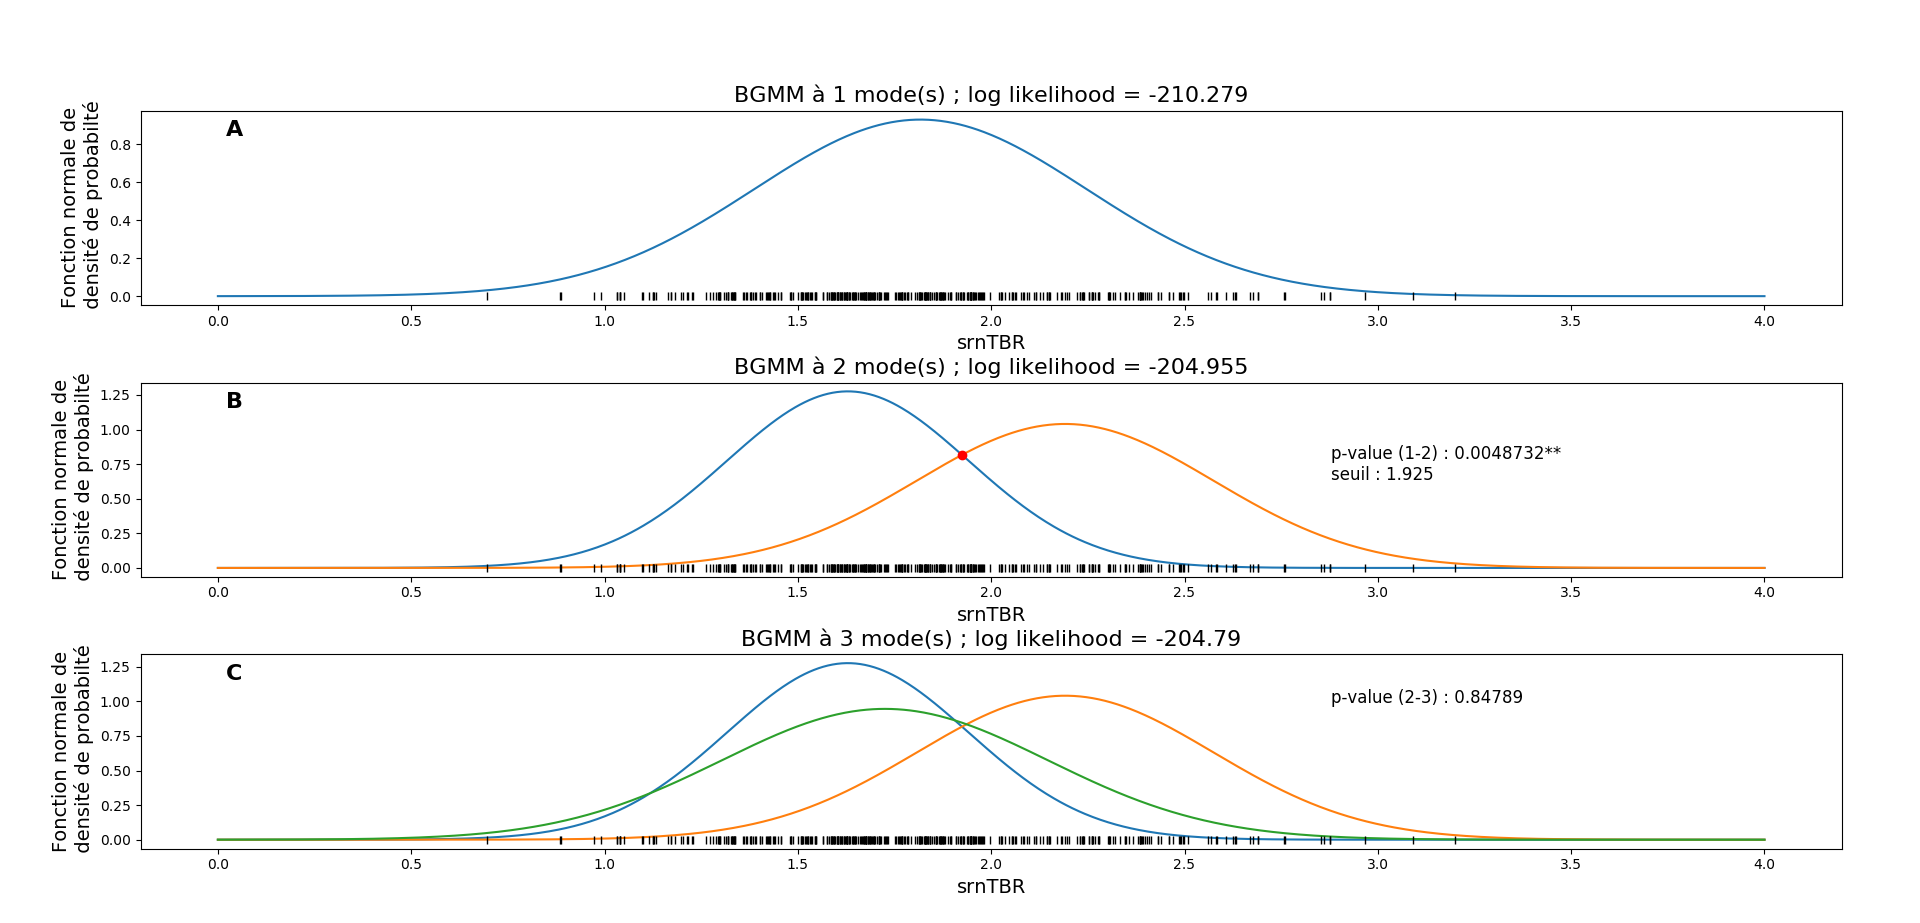
\includegraphics[width=1.0\linewidth]{figures/chapter-4/tbr-bgmm} 
  \caption{Tracés des distributions de \gls{srntbr} (\textit{rug plot}) avec \textbf{A)} 1-mode, \textbf{B)} 2-modes et \textbf{C)} 3-modes du \gls{bgmm} superposés. P-value (1-2) correspond
	à la p-value du test de déviance comparant les 1-mode et 2-modes du \gls{bgmm} ; p-value (2-3) correspond à la p-value du test de déviance comparant les 2-modes et 3-modes du \gls{bgmm}. 
	Significativité symbolisée par ** (seuil fixé à 0.01). Le seuil \gls{srntbr} est précisé pour le modèle à 2 composantes et représenté par un cercle rouge.}
  \label{Figure:tbr_bgmm} 
\end{figure}

Une différence statistiquement significative est observée dans la modélisation des distributions entre les modes à 1 (modèle nul) et à 2 composantes 
du \gls{bgmm} (p-value = 0.005), alors qu'aucune différence statistiquement significative n'est observée entre les modes à 2 (modèle nul) 
et à 3 composantes du \gls{bgmm} (p-value = 0.850). On peut donc en conclure que le \gls{bgmm} à deux modes décrit mieux la donnée que les deux
autres modes. 

Le \gls{gmm} arrive à la même conclusion : la distribution des \gls{srntbr} semble bimodale (p-value pour la comparaison
entre le modèle à 1 mode (modèle nul) et à 2 modes = 0.002). Ainsi, les \textit{a priori} utilisés pour le \gls{bgmm} semblent bien 
représenter la donnée. 

\subsubsection{Méthode de Ward}
Tout d'abord, les résultats d'un partitionnement suivant la méthode de Ward sont représentés sur un dendrogramme Figure~\ref{Figure:tbr_ward_dendrogram} :

\begin{figure}[h!]
  \centering
	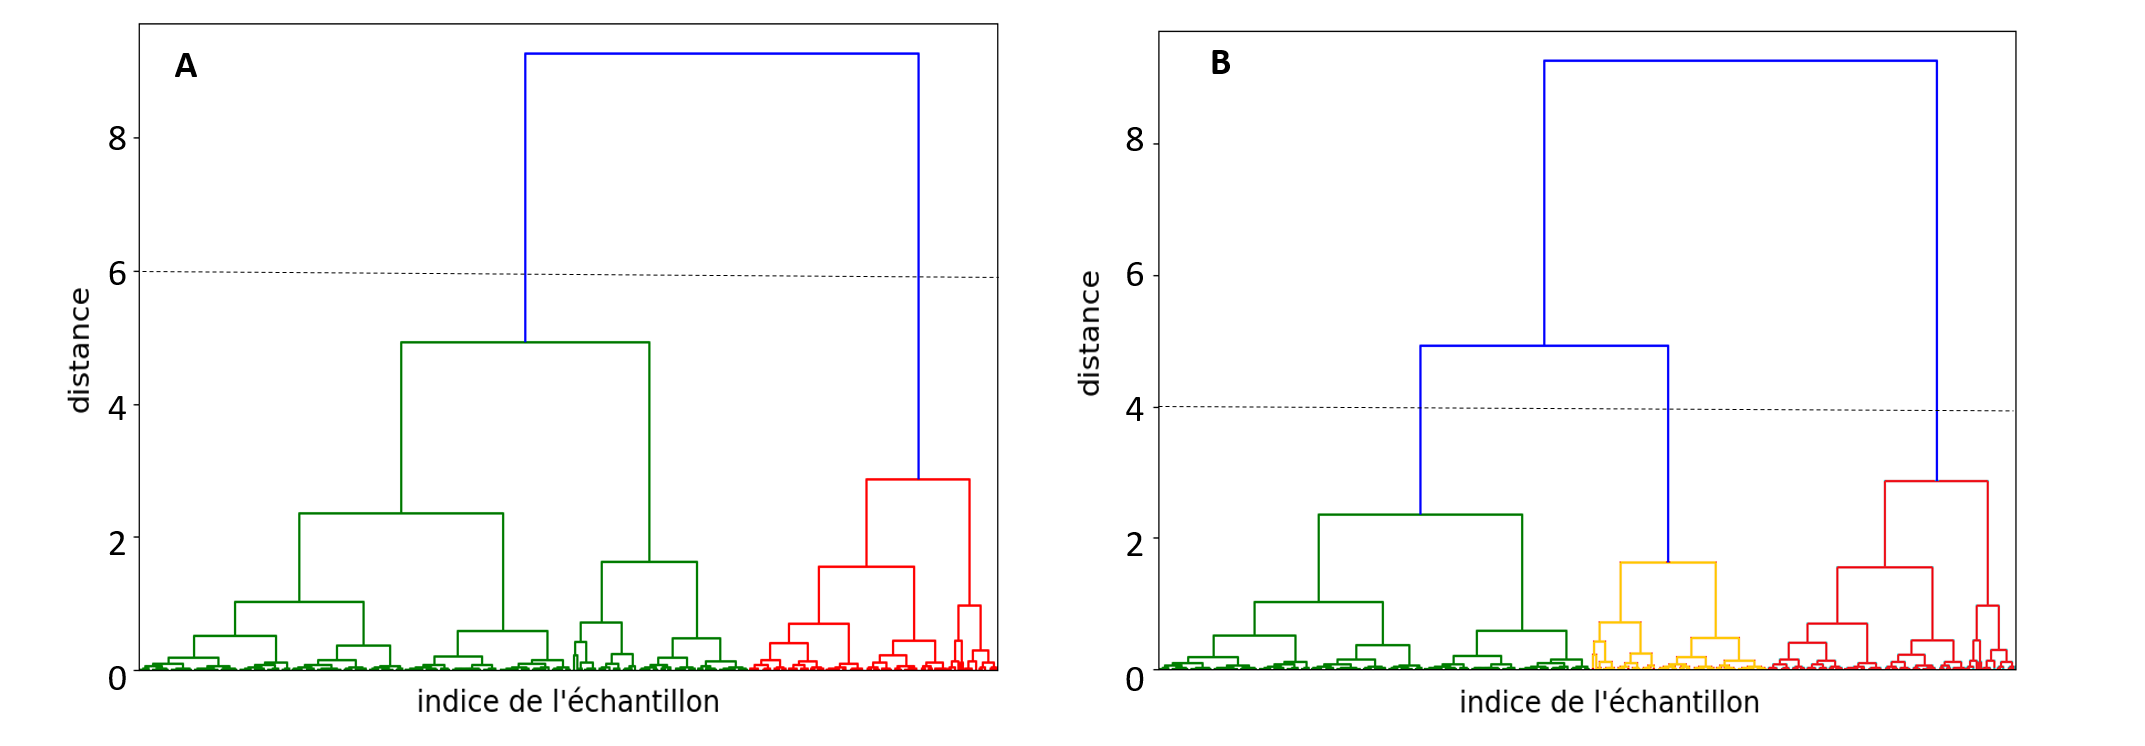
\includegraphics[width=1.0\linewidth]{figures/chapter-4/tbr-dendrogram-ward} 
  \caption{Dendrogramme représentant le partitionnement obtenu suivant la méthode de Ward. Tous les liens connectant des noeuds avec des distances plus 
	grandes ou égales à un seuil fixé à 6 sont colorés en bleu. Les deux clusters définis par les deux noeuds en dessous de ce seuil de 6 sont colorés différemment.}
  \label{Figure:tbr_bgmm}
\end{figure}

Visuellement, la Figure~\ref{Figure:tbr_ward_dendrogram} permet de supposer que les données pourraient \textit{clusters} (en rouge et vert) e

\subsubsection{DBSCAN}

\subsection{Seuils identifiés}
% expliquer qu'on met le seuil au carré faire une ref aux figures où le seuil est écrit. Rajouter sur la figure des plots glmm l'intersection
% qui correspond au seuil
Le seuil qui sépare le plus précisément les deux \textit{clusters} du \gls{bgmm} à deux composantes est de 1.925 pour les valeurs \gls{srntbr},
ce qui correspond pour les valeurs \gls{tbr} à un seuil de 3.7.

Le seuil \gls{tbr} obtenu avec le \gls{gmm} à deux modes est de 3.8. 

\section{Discussion}

\subsection{Groupes et seuils identifiés}

\subsection{Analyse des facteurs de confusion}

\subsubsection{Correction des artefacts oculaires}

\subsubsection{Influence de l'âge}

\newpage
\chapter{Conclusion et perspectives} \label{chapitre-5}

\section{Conclusion}

Cette thèse avait pour but d'étudier les facteurs de réussite de l'entrainement par \gls{nfb} appliqué aux enfants \gls{tdah} et, pour ce faire, trois objectifs ont été identifiés :
\begin{enumerate}
\item étudier l'efficacité du \gls{nfb} à l'aide d'une méta-analyse,
\item déterminer les paramètres inhérents à la mise en place du traitement par \gls{nfb} qui influencent sa performance,
\item analyser la distribution du \gls{tbr} au sein d'une population d'enfants \gls{tdah} pour évaluer la pertinence de la personnalisation du \gls{nfb}.
\end{enumerate}

Pour atteindre le premier objectif, la méta-analyse la plus récente au moment où ce travail a été réalisé, celle de \citep{Cortese2016}, a été répliquée et mise à jour à l'aide d'un package
Python développé dans le cadre de cette thèse. Les résultats de cette première étape confirment ceux obtenus par \citep{Cortese2016} : les parents, qui savent quel traitement suivent leurs enfants, 
observent une amélioration de leurs symptômes, ce qui n'est pas le cas des enseignants, qui eux sont considérés comme probablement aveugles au traitement. Toutefois, lorsqu'on étudie
précisément l'évolution de l'\glsfirst{est} et de sa $p$-value au fur et à mesure de l'inclusion des études selon leur année de publication, on remarque que ces valeurs ne se sont pas 
stabilisées, ce qui appelle à de nouvelles mises à jour. 

Ce travail a été l'occasion d'explorer 
la littérature sur le \gls{nfb} et ainsi de souligner l'hétérogénéité des choix cliniques, méthodologiques et techniques effectués dans les études d'efficacité qui impactent la fiabilité
des résultats obtenus dans les méta-analyses. C'est pourquoi une approche tirant avantage de cette hétérogénéité a été mise en place : la \gls{saob}.

La \gls{saob} a recours à des méthodes multivariées pour déterminer les facteurs cliniques, méthodologiques et/ou techniques qui pourraient avoir une influence sur l'efficacité du \gls{nfb}. 
Cette analyse permet de conclure qu'un traitement intensif (c'est à dire court mais avec un rythme important de sessions par semaine) augmenterait l'efficacité du \gls{nfb}. A l'inverse,  
intégrer une phase de transfert durant la session diminuerait son efficacité. Par ailleurs, comme attendu, les évaluations des enseignants ne sont pas en faveur de l'efficacité du \gls{nfb}, 
ce qui est en accord avec les résultats des méta-analyses. Cette différence entre ces deux types d'évaluateurs 
peut, à première vue, s'expliquer par l'effet placebo. Cependant, il semblerait plutôt que les enseignants détecteraient moins de symptômes chez les enfants, ce qui remettrait en question la
pertinence de les utiliser pour quantifier l'effet placebo. Ici aussi, la mise à jour de ces résultats est nécessaire : plus la \gls{saob} sera appliquée sur un nombre important d'observations,
plus ses résultats seront fiables

La \gls{saob} a permis d'étudier l'impact de différents facteurs sur la performance du \gls{nfb}, cependant la personnalisation des protocoles d'entrainement dont l'influence serait intéressante 
à explorer, a été exclu de cette analyse, faute d'un nombre suffisant d'études la proposant. Ainsi, la pertinence de la personnalisation du \gls{nfb} a été étudiée ici grâce à l'analyse de la distribution 
du \gls{tbr} chez une large population d'enfants \gls{tdah}. Trois méthodes de partionnement se sont accordées sur le fait que cette distribution est bimodale, ce qui va dans 
le sens d'une personnalisation de protocoles basée la valeur de \gls{tbr} dont la valeur seuil conduisant au meilleur équilibre entre \gls{fpr} et \gls{tpr} est de 4.1. 

Ainsi, le travail présenté dans ce manuscrit a permis de décrire avec précision comment l'efficacité du \gls{nfb} est évaluée à l'aide de la technique de la méta-analyse et de donner des 
directions pour choisir les paramètres permettant d'obtenir une meilleure performance du \gls{nfb}.


\section{Perspectives}

Les résultats présentés ici, notamment ceux de la méta-analyse et de la \gls{saob}, ont vocation à être mis à jour afin d'inclure davantage d'études : les résultats alors obtenus se 
stabiliseront et leur fiabilité augmentera.   

Par ailleurs, de nouveaux facteurs pourront être étudiés avec la \gls{saob}, apportant ainsi de nouvelles  
indications. Dans sa forme actuelle, la \gls{saob} donne des indications qualitatives sur comment choisir les facteurs, il serait peut-être intéressant de mettre en place des
méthodes conduisant à des directives qualitatives.

Les conclusions de l'analyse de la distribution des valeurs de \gls{tbr} issues d'une large population d'enfants \gls{tdah} justifierait le recours à la 
personnalisation des protocoles de \gls{nfb} selon le profil \gls{eeg} de l'enfant. Ce genre d'approche est de plus en plus utilisée, ainsi davantage d'analyses s'intéressant
à la pertinence et à l'efficacité d'une telle approche vont être menées : il serait notamment important de déterminer si l'âge des enfants a effectivement influencé l'étude
présentée dans ce manuscrit. Par ailleurs, appliquer ces analyses sur des valeurs de \gls{tbr} obtenues les yeux fermés serait à envisager. 

Enfin, dans ce manuscrit, le \gls{nfb} a été étudié pour les enfants souffrant du \gls{tdah} mais les analyses effectuées ici pourraient être 
transposées à une toute autre application comme celles listées en \ref{NFB_applications}.
En particulier, la \gls{saob} pourrait être adaptée, c'est à dire ne pas étudier les facteurs propres au \gls{nfb} 
appliqué au \gls{tdah}, de façon à inclure toutes les études sur l'efficacité du \gls{nfb} 
quel que soit le trouble à traiter, pour déterminer si des facteurs généraux sont identifiés comme sugéré en \ref{conclusion_saob}. 


\newpage
\fancyhead[RO]{Bibliographie}
\bibliography{bibliography}

\newpage
\thispagestyle{empty}

\end{document}